\documentclass[a4paper, 12pt, twoside]{article}

\usepackage{latexki}

\lecturer{Prof. Dr. F. Herrlich}
\semester{Wintersemester 06/07}
\scriptstate{unknown}

\usepackage{grugraStyle}

\title{Gruppen und Graphen}
\date{}

\setcounter{tocdepth}{2}

\makeindex

% --------------------
\begin{document}

\thispagestyle{empty}
\begin{center}
\Huge \textbf{\textsf{Gruppen und Graphen}}
\end{center}
\vspace{2cm}
\begin{center}
	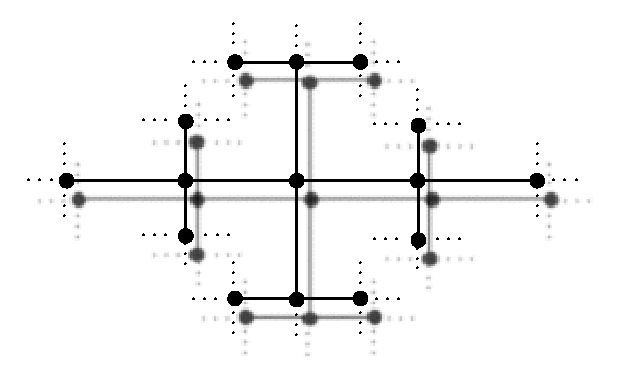
\includegraphics{grugraImages/titel}
\end{center}

\newpage

\renewcommand{\thepage}{\roman{page}} 

% sonstiges:
\newpage \thispagestyle{empty}
{\footnotesize
\vspace*{\stretch{2}}
Fassung vom \today.

Zum Erstellen der Grafiken wurden die Programme {\sf OmniGraffle} und
{\sf MuPAD} verwendet.
}
\cleardoublepage

\tableofcontents
\cleardoublepage

\setcounter{page}{1} % jetzt gehts los, arabische Ziffern
\renewcommand{\thepage}{\arabic{page}} 

\cleardoublepage
\part{Graphen und Bäume}

% ===============
\section{Graphen}\label{sec_graphen}

\DEF Ein \emph{Graph}\index{Graph} $\GR$ besteht aus zwei Mengen
\begin{align*}
& E=E(\GR) \quad \text{(die \emph{Ecken}\index{Ecke} von $\GR$)} \\
& K=K(\GR) \quad \text{(die \emph{orientierten Kanten}\index{Kante}\index{orientierte Kanten}\index{Kante!orientiert} von $\GR$)}\index{$\GR$ (Graph)}\index{$E(\GR)$ (Ecken)}\index{$K(\GR)$ (Kanten)}\index{$\ini(k)$, $\ter(k)$}
\end{align*}
und den Abbildungen
\[
I : K \Ra E\times E,\quad k \mapsto (\ini(k),\ter(k))
\]
und
\[
\bar{\ }:K\Ra K,\quad k\mapsto\bar{k},
\]
mit den Eigenschaften
\begin{enumerate}
\item $k\neq \bar{k}$ für alle $k\in K$,
\item $\bar{\bar{k}}=k$ für alle $k\in K$,
\item $\ini(\bar{k})=\ter(k)$ für alle $k\in K$ (dann gilt auch $\ter(\bar{k})=\ini(k)$).
\end{enumerate}
Ein Paar $\{k,\bar{k}\}$ heißt \emph{geometrische Kante}\index{Kante!geometrisch}.
Als \emph{Orientierung}\index{Orientierung} eines Graphen bezeichnen
wir die Wahl einer Teilmenge $K^+ \subset K$, so dass
$k\in K^+$ genau dann, wenn
$\bar{k}\in K^- := K\backslash K^+$ ist.\index{$K(\GR)^+$, $K(\GR)^-$ (Orientierung)}

Mengenoperationen auf Graphen sind immer auf den entsprechenden
Mengen $E$ und $K$ zu verstehen.

\BSP Graphen.
\begin{center}
	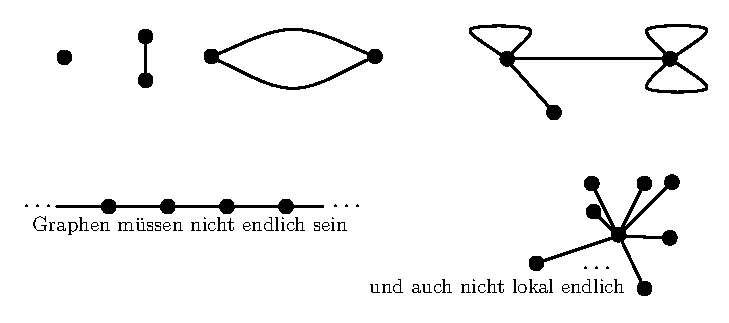
\includegraphics{grugraImages/bspgraphen}
\end{center}

\BEM $\GR$ kann \glqq topologisiert\grqq\ werden:
Geometrische Kanten werden mit $[0,1]$ identifiziert und verklebt,
wenn sie gemeinsame Ecken haben. Es ist sogar möglich, jeden
Graphen als Teilraum von $\RR^3$ zu realisieren, i.A. ist es aber nicht möglich, einen Graphen als Teilraum von $\RR^2$ zu realisieren
(siehe etwa Kapitel 3 in Diestel \cite{diestel}).

\DB Es seien $\GR=(E,K,I)$ und $\GR'=(E',K',I')$ Graphen.
\begin{enumerate}
\item Ein \emph{Morphismus}\index{Morphismus} $f:\GR\Ra\GR'$ ist ein
Paar $f=(f_E,f_K)$ von Abbildungen
$f_E:E\Ra E'$ und $f_K:K\Ra K'$ mit
\[
I'(f_K(k)) = ( f_E(\ini(k)), f_E(\ter(k)) )
= (f_E \times f_E)(I(k))
\]
und
\[
f_K(\bar{k}) = \bar{f_K(k)}
\]
für alle $k\in K$.
\item Die Komposition zweier Morphismen $f,g$
\[
f\circ g = (f_E\circ g_E, f_K\circ g_K),
\]
ist wieder ein Morphismus.
\item $f$ heißt \emph{Isomorphismus}\index{Isomorphismus}, wenn es
einen Morphismus $g:\GR'\Ra\GR$ gibt mit
\[
f\circ g = \id_{\GR'} \text{ und } g\circ f=\id_{\GR}.
\]
Ein Isomorphismus $f:\GR\Ra\GR$ heißt \emph{Automorphismus}\index{Automorphismus}.
\item $f$ ist genau dann ein Isomorphismus, wenn $f_E$ und $f_K$
bijektiv sind.
\end{enumerate}

\DB Es sei $\GR$ ein Graph.
\begin{enumerate}
\item Ein \emph{Weg}\index{Weg} $w$ (der Länge $|w|=n\geq 0$) in $\GR$
ist eine Folge
\[
w = (k_1,\ldots,k_n)
\]
von Kanten $k_i\in K(\GR)$ mit $\ter(k_i)=\ini(k_{i+1})$ für
$i=1,\ldots,n-1$.
\[
\ini(w):=\ini(k_1) \text{ und } \ter(w):=\ter(k_n)
\]
heißen \emph{Anfangs-} und \emph{Endpunkt} von $w$.\index{Anfangspunkt}\index{Endpunkt}
Ist $n=0$, so wird $\ini(w)=\ter(w)\in E(\GR)$ definiert.
\item Setze
\begin{center}
	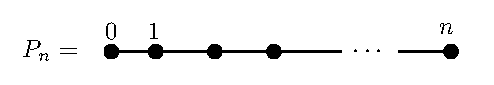
\includegraphics{grugraImages/Pn}
\end{center}
(fester Graph mit $n+1$ Ecken und $2n$ Kanten) und $w$ der stachelfreie Weg mit
$\ini(w)=0 \text{ und } \ter(w)=n$. Dann ist jeder Weg der Länge $n$ in $\GR$ das Bild
von $w$ unter einem Morphismus $P_n\Ra \GR$.
\item $\GR$ heißt \emph{zusammenhängend}\index{zusammenhängend!Graph}\index{Graph!zusammenhängend},
wenn es für alle $x,y\in E(\GR)$ einen Weg in $\GR$ gibt mit
$\ini(w)=x$ und $\ter(w)=y$.
\item Ein Weg heißt \emph{stachelfrei}\index{stachelfreier Weg}\index{Weg!stachelfrei},
wenn $k_{i+1}\neq \bar{k}_i$ ist für $i=1,\ldots,n-1$.
\item Gibt es in $\GR$ einen Weg von $x$ nach $y$, so gibt es auch
einen stachelfreien Weg.
\end{enumerate}
\textsc{Beweis von 5.:} Es sei $w=(k_1,\ldots,k_n)$ und
$k_{i+1}=\bar{k}_i$. Dann gilt:
\[
\ini(k_{i+2}) = \ter(k_{i+1}) = \ter(\bar{k}_{i})
= \ini(k_i) = \ter(k_{i-1}).
\]
Folglich ist $w'=(k_1,\ldots,k_{i-1},k_{i+2},\ldots,k_n)$ ein
Weg von $x$ nach $y$.
\qed

\DB Es sei $\GR$ ein Graph.
\begin{enumerate}
\item Ein Weg $w$ in $\GR$ heißt \emph{geschlossen}\index{geschlossener Weg}\index{Weg!geschlossen},
wenn $\ini(w)=\ter(w)$.
\item $w$ heißt \emph{einfach}\index{einfacher Weg}\index{Weg!einfach},
wenn $\ini(k_i)\neq\ini(k_j)$ für $i\neq j$.
\item Einfache Wege sind insbesondere auch stachelfrei (für Wege
der Länge $2$ ist dies als Definition zu verstehen).
\item Ein einfacher geschlossener Weg der Länge $n\geq 1$ heißt
\emph{Kreis}\index{Kreis}\index{Weg!Kreis}.
Ein Kreis der Länge $1$ heißt \emph{Schleife}\index{Schleife}\index{Weg!Schleife}\index{Kreis!Schleife}.
\begin{center}
	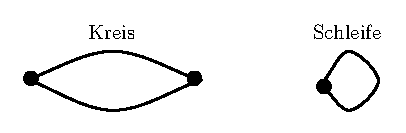
\includegraphics{grugraImages/kreis}
\end{center}
\item Ein Paar $k_1\neq k_2$ von Kanten in $\GR$ heißt \emph{Doppelkante}\index{Doppelkante}\index{Kante!Doppel-},
wenn $\ini(k_1)=\ini(k_2)$ und $\ter(k_1)=\ter(k_2)$ ist.
\begin{center}
	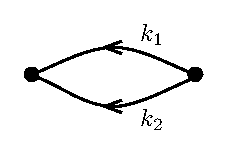
\includegraphics{grugraImages/doppelkante}
\end{center}
\item Ein Graph heißt \emph{kombinatorisch}\index{kombinatorischer Graph}\index{Graph!kombinatorisch},
wenn er keine Schleifen und keine Doppelkanten enthält.
\item Ein Graph ist genau dann kombinatorisch, wenn er als
topologischer Raum ein simplizialer Komplex ist.\index{simplizialer Komplex}
\end{enumerate}

\DB Es sei $\GR$ ein zusammenhängender Graph. Für $x,y\in E(\GR)$ sei
\[
d(x,y) := \min\{ n : \text{ es gibt einen Weg $w$ von $x$ nach $y$
	mit $|w|=n$} \}.
\]\index{$d(x,y)$ (Metrik)}
Dann ist $d$ eine Metrik\index{Metrik} auf $\GR$
(genauer: auf $E(\GR)$).
Der \emph{Durchmesser}\index{Durchmesser}\index{$d(\GR)$ (Durchmesser)}
von $\GR$ ist
\[
d(\GR) := \sup\{ d(x,y) : x,y\in E(\GR)\}.
\]

%==============================
\section{Bäume}\label{sec_baum}

\DEF Ein \emph{Baum}\index{Baum}\index{Graph!Baum} ist ein
zusammenhängender Graph ohne Kreise.

\BSP Bäume.
\begin{center}
	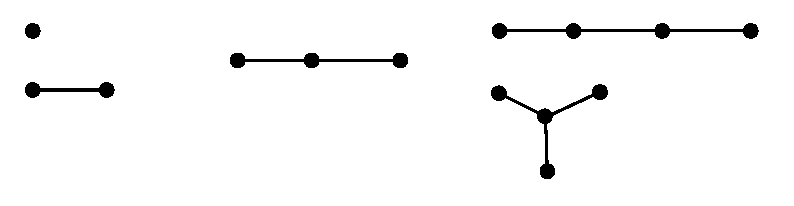
\includegraphics{grugraImages/bspbaum}
\end{center}

\PROP Ein Graph $\GR$ ist genau dann ein Baum, wenn es zu je zwei
seiner Ecken $x,y$ genau einen stachelfreien Weg von $x$ nach $y$ in
$\GR$ gibt.

\bew \glqq$\ra$\grqq: Seien $x,y\in E(\GR)$,
$w=(k_1,\ldots,k_n)$ und $w'=(k'_1,\ldots,k'_m)$ stachelfreie Wege
von $x$ nach $y$. Ist $k_n\neq k'_m$, so ist
$\tilde{w}=(k_1,\ldots,k_n,\bar{k}'_m,\ldots,\bar{k}'_1)$
ein stachelfreier geschlossener Weg, enthält also einen
Kreis, im Widerspruch dazu, dass $\GR$ ein Baum ist.
Also muss $k_n=k'_m$ sein. Induktion über die Weglänge $n$ ergibt
die Behauptung.

\glqq $\la$\grqq: Da es zwischen je zwei Ecken einen Weg gibt, ist
$\GR$ zusammenhängend. Da es genau einen Weg gibt, kann es keine
Kreise geben.
\qed

\DB Sei $\GR$ ein Graph und $x\in E(\GR)$.
\begin{enumerate}
\item Es sei
\[
K_x := \{ k\in K(\GR) : \ini(k)=x \}.
\]
Die \emph{Ordnung}\index{Ordnung}\index{$v(x)$ (Valenz)} von $x$ ist
\[
v(x) := |K_x|.
\]
(Die Ordnung wird auch als \emph{Valenz}\index{Valenz (siehe Ordnung)}
oder \emph{Index} \index{Index (siehe Ordnung)} von
$x$ bezeichnet.)
\item $x$ heißt \emph{Endpunkt}\index{Endpunkt}, wenn $v(x)=1$ ist.
Es bezeichne $\ep(\GR)$\index{$\ep(\GR)$ (Endpunkte)} die Menge der Endpunkte von $\GR$.
\item $\GR-x$\index{$\GR-x$} sei der Graph mit $E(\GR-x)=E(\GR)\backslash\{x\}$
und $K(\GR-x)=K(\GR)\backslash(K_x\cup \bar{K}_x)$
(Entfernen des \glqq Sterns\grqq\ um $x$). $\GR-x$ ist ein Teilgraph
von $\GR$.
\item Ist $x$ ein Endpunkt, so gilt:
\begin{enumerate}
	\item $\GR$ ist genau dann zusammenhängend, wenn $\GR-x$
	zusammenhängend ist.
	\item Jeder Kreis in $\GR$ ist in $\GR-x$ enthalten.
	\item $\GR$ ist genau dann ein Baum, wenn $\GR-x$ ein Baum ist.
\end{enumerate}
\end{enumerate}
\textsc{Beweis von 4.:} (a) und (b) sind klar und ergeben
zusammen (c).
\qed

\PROP\
\label{prop_fix}
\begin{enumerate}
\item Sei $f:\GR\Ra\GR'$ ein Isomorphismus von Graphen.
Dann gilt
\[
v(x) = v(f_E(x))
\]
für alle $x\in E(\GR)$.
\item Es sei $\GR'=\GR-\ep(\GR)$. Jeder Automorphismus von $\GR$
induziert einen Automorphismus von $\GR'$.
\item Ist $\GR$ ein Baum von endlichem Durchmesser $n=d(\GR)$,
so gibt es für
	\begin{itemize}
	\item gerades $n$ eine Ecke $x\in E(\GR)$ mit $f_E(x)=x$
	\item ungerades $n$ eine geometrische Kante $\kappa=\{k,\bar{k}\}$
	mit $f_K(\kappa)=\kappa$
	\end{itemize}
für jeden Automorphismus $f$ von $\GR$.
\end{enumerate}
\bew 
\begin{enumerate}
\item $f_K$ induziert eine Bijektion $K_x\Ra K'_{f_E(x)}$.
\item Folgt aus 1.
\item Für $n=0$ und $n=1$ ist die Aussage klar.\\
Wir zeigen im Folgenden, dass $\GR'=\GR-\ep(\GR)$ ein Baum vom
Durchmesser $n-2$ ist (falls $n\geq 2$), dann folgt die
Behauptung durch Induktion über $n$.\\
Es sei $w'=(k'_1,\ldots,k'_m)$ ein stachelfreier Weg in $\GR'$
und $x=\ini(w')$, $y=\ter(w')$. Dann ist $m=d(x,y)$.
Da in $\GR$ gilt $v(x)\geq 2$, $v(y)\geq 2$, gibt es eine Kante
$k_1\neq k'_1$ in $\GR$ mit $\ini(k_1)=x$ und eine Kante
$k_m\neq \bar{k}'_m$ in $\GR$ mit $\ini(k_m)=y$.
Dann ist $w=(\bar{k}_1,k'_1,\ldots,k'_m,k_m)$ ein stachelfreier Weg
in $\GR$. Es ist also $m+2\leq d(\GR)$ und somit $m\leq n-2$.\\
Sei umgekehrt $w=(k_1,\ldots,k_n)$ ein stachelfreier Weg in $\GR$.
Für $i=2,\ldots,n$ ist $v(\ini(k_i))\geq 2$. Folglich ist
$(k_2,\ldots,k_{n-1})$ ein stachelfreier Weg in $\GR'$.
Somit gilt auch $d(\GR')\geq n-2$.
\qed
\end{enumerate}

\BSP Der endliche Durchmesser ist in Teil 3. von Proposition
\ref{prop_fix} wesentlich, wie das Beispiel einer (in beiden
Richtungen) unendlichen Kette\index{unendliche Kette} zeigt:
\begin{center}
	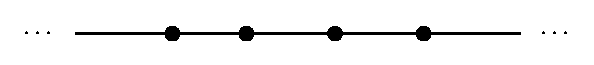
\includegraphics{grugraImages/unendldiam}
\end{center}
ist ein Baum von unendlichem Durchmesser. Hier ist eine Translation
ein Automorphismus ohne Fixpunkt und Fixkante.

\FOLG \label{folg_endpkt}
Jeder endliche Baum entsteht aus $\bullet$ durch wiederholtes
Anhängen von Endpunkten.

\DB Es sei $\GR$ ein Graph.
\begin{enumerate}
\item Ein Teilbaum $T\subset \GR$ heißt \emph{aufspannend}\index{aufspannender Baum}\index{Baum!aufspannend}
(oder auch \emph{Gerüst}\index{Gerüst}), wenn $E(T)=E(\GR)$ ist.
\item Jeder zusammenhängende Graph besitzt einen aufspannenden
Teilbaum.
\end{enumerate}
\bew
Es sei $T_0\subset \GR$ ein Teilbaum. Ist $E(T_0)\neq E(\GR)$,
so gibt es eine Kante $k\in K(\GR)$ mit
$\ini(k)\in E(T_0)$ und $\ter(k)\not\in E(T_0)$.
Dann ist $T' := T_0\cup\{k,\bar{k},\ter(k)\}$ ein Teilbaum von
$\GR$.\\
Ist $\GR$ endlich, so erhalten wir mit Induktion einen
Teilbaum $T$ mit $E(T)=E(\GR)$.\\
Falls $\GR$ nicht endlich ist, betrachte die Menge $\calT$ der
Teilbäume von $\GR$. Es ist $\calT\neq\emptyset$ und $\calT$
ist durch die Teilbaumrelation partiell geordnet.
Ist $T_1\subset T_2\subset \cdots$ eine austeigende Kette von
Teilbäumen, so ist $\bigcup_i T_i \in \calT$.
Nach dem Zornschen Lemma muss es also ein maximales Element
$T\in \calT$ geben.
Angenommen $E(T)\neq E(\GR)$. Dann könnte man wie im endlichen Fall
einen Baum $T'\supsetneq T$ konstruieren, im Widerspruch zur
Maximalität von $T$.
\qed

\DB \label{bem_geschlecht}
Sei $\GR$ ein endlicher zusammenhängender Graph.
Wir setzen
\begin{align*}
&e(\GR) := |E(\GR)|,\\
&k(\GR) := \frac{1}{2}|K(\GR)|.
\end{align*}
Das \emph{Geschlecht}\index{Geschlecht}\index{$g(\GR)$ (Geschlecht)}\index{$e(\GR)$, $k(\GR)$}
von $\GR$ ist
\[
g(\GR) := k(\GR) - e(\GR) + 1.
\]
Das Geschlecht wird auch als \emph{zyklomatische Zahl}\index{zyklomatische Zahl (siehe Geschlecht)}
oder \emph{Betti-Zahl}\index{Betti-Zahl (siehe Geschlecht)}
bezeichnet.
Es gilt:
\begin{enumerate}
\item $g(\GR) \geq 0$.
\item $g(\GR) = 0$ genau dann, wenn $\GR$ ein Baum ist.
\end{enumerate}
\bew Ist $\GR$ ein Baum, so ist nach Folgerung \ref{folg_endpkt}
$g(\GR)=0$. Ist $\GR$ kein Baum, so sei $T$ ein aufspannender Baum
von $\GR$. Also ist $e(\GR)=e(T)$ und $k(\GR)>k(T)$ und damit
$g(\GR)>g(T)=0$.
\qed

\DB Sei $\GR$ ein Graph und $Z$ ein zusammenhängender Teilgraph.
Mit $\GR/Z$\index{$\GR/Z$ (Kontraktion)} bezeichnen
wir den folgenden Graphen
\begin{align*}
E(\GR/Z) &= ( E(\GR)-E(Z) )\cup\{z\},\\
K(\GR/Z) &= K(\GR)-K(Z),\\
I_{\GR/Z}(k) &= (\ini_{\GR/Z}(k),\ter_{\GR/Z}(k)), \quad k\in K(\GR/Z).
\end{align*}
mit
\[
\ini_{\GR/Z}(k) =
\left\{\begin{matrix}
\ini(k), & \ini(k)\not\in E(Z),\\
z, & \ini(k)\in E(Z)
\end{matrix}\right.
\quad
\text{ und }
\quad
\ter_{\GR/Z}(k) =
\left\{\begin{matrix}
\ter(k), & \ter(k)\not\in E(Z),\\
z, & \ter(k)\in E(Z)
\end{matrix}\right.
.
\]
\begin{center}
	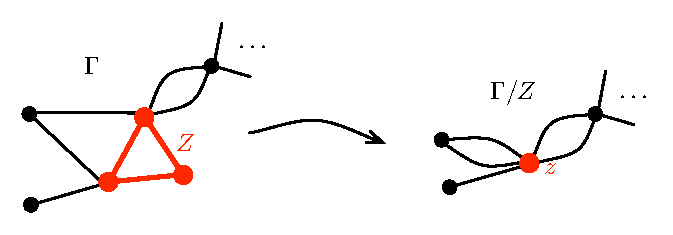
\includegraphics{grugraImages/GZ1}
\end{center}

\BSP Ist $Z$ ein Gerüst von $\GR$, so erhalten wir
\begin{center}
	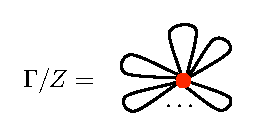
\includegraphics{grugraImages/GZ2}
\end{center}
mit $g(\GR)$ Kanten.

\DEF
Wir sagen, dass $\GR/Z$ aus $\GR$ durch \emph{Kontraktion}\index{Kontraktion}
von $Z$ entsteht.
Ist $Z$ nicht zusammenhängend, so wird $\GR/Z$ durch Kontraktion
jeder Zusammen\-hangskomponente von $Z$ definiert.

\BEM \label{bem_GZ}
Ist $\GR$ ein endlicher zusammenhängender Graph und $Z$ ein
Teilgraph, so gilt:
\begin{enumerate}
\item $g(\GR/Z) \leq g(\GR)$.
\item $g(\GR/Z) = g(\GR)$, falls $Z$ ein Teilbaum ist.
\end{enumerate}

\DEF Ein Graph, dessen Zusammenhangskomponenten Bäume sind,
heißt \emph{Wald}\index{Wald}.

\PROP\label{prop_wald}
Es sei $\GR$ ein zusammenhängender Graph und $Z$ ein Teilwald
von $\GR$. Dann ist $\GR/Z$ genau dann ein Baum, wenn $\GR$ ein
Baum ist.

\bew Ist $\GR$ endlich, so folgt die Behauptung aus Bemerkung
\ref{bem_GZ} und Bemerkung \ref{bem_geschlecht}.
Ist $\GR$ unendlich, so sei $\GR'$ ein endlicher zusammenhängender
Teilgraph von $\GR$. Dann ist $\GR'\cap Z$ ein endlicher Wald.
Also ist $\GR'$ ein Baum, genau dann wenn $\GR'/(\GR'\cap Z)$ ein Baum
ist. Schöpfe nun $\GR$ durch endliche Teilgraphen aus.
\qed


\cleardoublepage
\part{Cayley-Graphen und Automorphismengruppen}

% =============
\section{Cayley-Graphen von Gruppen}\label{sec_cayley}

\BEM\
\begin{enumerate}
\item Für jeden Graphen $\GR$ bildet die Menge $\Aut(\GR)$ der
Automorphismen von $\GR$ eine Gruppe.\index{Automorphismengruppe}\index{Gruppe!Automorphismen}\index{$\Aut(\GR)$}
\item $\Aut(\GR)$ ist eine Untergruppe von
$\perm(E(\GR)) \times \perm(K(\GR))$.
\item Ist $\GR$ ein kombinatorischer Graph, so ist
$\Aut(\GR)\leq \perm(E(\GR))$.
\end{enumerate}

\BSP Automorphismengruppen von Graphen.
\begin{enumerate}
\item Für
\begin{center}
	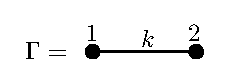
\includegraphics{grugraImages/aut1}
\end{center}
ist $\Aut(\GR)=\{\id,\sigma\}\cong \ZZ/2\ZZ$ mit
$\sigma(1)=2$, $\sigma(2)=1$ und $\sigma(k)=\bar{k}$.
\item Für
\begin{center}
	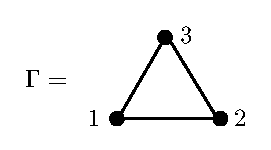
\includegraphics{grugraImages/aut2}
\end{center}
besteht $\Aut(\GR)$ aus allen Permutationen der drei Ecken,
also ist $\Aut(\GR)\cong \sym_3$.
\item Für
\begin{center}
	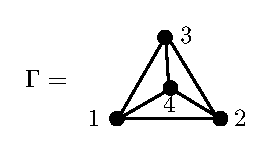
\includegraphics{grugraImages/aut3}
\end{center}
ist $\Aut(\GR)\cong \sym_4$.
\item Die Automorphismengruppe von
\begin{center}
	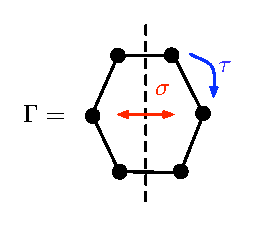
\includegraphics{grugraImages/aut4}
\end{center}
enthält sechs Drehungen drei Spiegelungen mit Spiegelachse
durch zwei Ecken und drei Spiegelungen mit Spiegelachse durch
Kantemittelpunkte, hat also mindestens zwölf Elemente.
In der Tat ist bereits
\[
\Aut(\GR) = \{\id,\tau,\ldots,\tau^5,
	\sigma,\sigma\tau,\ldots,\sigma \tau^5 \}
\cong \mathrm{D}_6.
\]
$\mathrm{D}_6$ ist die Diedergruppe des Sechsecks.\index{Diedergruppe}
\end{enumerate}

\DB Es sei $G$ eine Gruppe und $S\subset G$.
Der \emph{Cayley-Graph}\index{Cayley-Graph}\index{Graph!Cayley-}\index{Gruppe!Cayley-Graph}
$\GR(G,S)$\index{$\GR(G,S)$ (Cayley-Graph)} von $G$ bzgl. $S$ wird wie folgt definiert:
\begin{align*}
E(\GR(G,S)) &:= G, \\
K(\GR(G,S)) &:= G \times S \times \{-1,1\},
\end{align*}
und für $k=(g,s,\eps)\in K(\GR(G,S))$ sei $\bar{k}=(g,s,-\eps)$
und
\begin{align*}
&\ini(k) = g, \quad \ter(k) = gs \quad \text{falls } \eps = 1, \\
&\ini(k) = gs, \quad \ter(k) = g \quad \text{falls } \eps = -1.
\end{align*}

\BSP\label{bsp_cay}
Cayley-Graphen.
\begin{enumerate}
\item Es sei $G$ beliebig, $S=\emptyset$.
Dann ist $K(\GR(G,S))=\emptyset$.
\item $G=\ZZ$ und $S=\{1\}$:
\begin{center}
	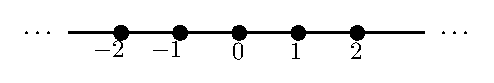
\includegraphics{grugraImages/cay1}
\end{center}
\item $G=\ZZ$ und $S=\{2\}$:
\begin{center}
	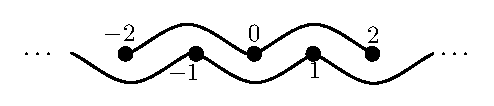
\includegraphics{grugraImages/cay3}
\end{center}
\item $G=\ZZ$ und $S=\{-1,1\}$:
\begin{center}
	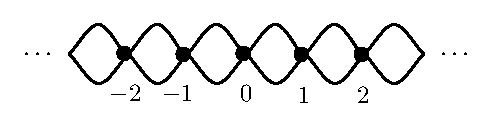
\includegraphics{grugraImages/cay2}
\end{center}
\item $G=\ZZ/n\ZZ$ und $S=\{1\}$:
\begin{center}
	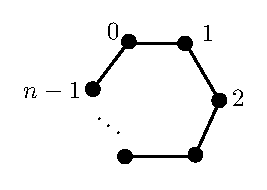
\includegraphics{grugraImages/cay4}
\end{center}
\item $G=\sym_3$ und $S=\{\tau=(1\ 2\ 3),\sigma=(1\ 2)\}$.
Es ist $\sym_3=\{\id,\tau,\tau^2,\sigma,\sigma\tau,\sigma\tau^2\}$.
\begin{center}
	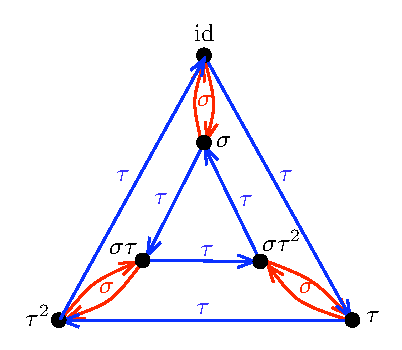
\includegraphics{grugraImages/cay5}
\end{center}
Man beachte, dass für die Kantenübergänge von rechts multipliziert 
wird.
\end{enumerate}

\BEM\label{bem_GRGS}\
\begin{enumerate}
\item $\GR(G,S)$ ist genau dann zusammenhängend, wenn
$G$ von der Menge $S$ erzeugt wird.
\item Für jede Ecke $g\in G=E(\GR(G,S))$ ist $v(g)=2|S|$.
\item $\GR(G,S)$ enthält genau dann Schleifen, wenn $1$ in $S$
enthalten ist.
\item $\GR(G,S)$ enthält genau dann Doppelkanten, wenn es in $S$
Elemente $s\neq 1$ gibt, so dass auch $s^{-1}\in S$ ist.
\item $\GR(G,S)$ enthält keine Dreifachkanten.
\end{enumerate}
\textsc{Beweis von 1.:} \glqq$\ra$\grqq: Sei $g\in G$ beliebig und
$w=(k_1,\ldots,k_n)$ ein Weg in $\GR(G,S)$ von $1$ nach $g$,
mit $k_i=(g_i, s_i, \eps_i)$. Dann ist
$g_1=1$, $g_2=s_1^{\eps_1}$, \ldots,
$g_n=s_1^{\eps_1}\cdots s_{n-1}^{\eps_{n-1}}$.
Somit ist $g=\ter(k_n)=g_n s_n^{\eps_n}=
s_1^{\eps_1}\cdots s_n^{\eps_n} \in\lag S\rag$.

\glqq $\la$\grqq: Führe die gleiche Überlegung rückwärts durch.
\qed

\DB Es sei $G$ eine Gruppe und $\GR$ ein beliebiger Graph.
\begin{enumerate}
\item Eine \emph{Aktion}\index{Aktion}\index{Gruppe!Aktion} (oder \emph{Operation}\index{Operation (siehe Aktion)}) von $G$ auf $\GR$ ist ein
Gruppenhomomorphismus $\rho:G\Ra\Aut(\GR)$.
\item Eine Aktion heißt \emph{treu}\index{Aktion!treu}\index{treue Aktion}
(oder \emph{effektiv}\index{effektiv (siehe treue Aktion)}\index{Aktion!effektiv}),
wenn $\K{\rho}=\{1\}$ ist. Der Kern von $\rho$ heißt auch
\emph{Ineffektivitätskern}\index{Ineffektivitätskern}
der Aktion $\rho$.
\end{enumerate}

\BEM Es sei $G$ eine Gruppe, $S\subset G$. Dann operiert $G$ von
links auf $\GR(G,S)$ und diese Operation ist treu.\\
Genauer: Für $g\in G$ sei $\phi_g:\GR(G,S)\Ra\GR(G,S)$ gegeben durch
\begin{align*}
\phi_g(g') &= gg', \\
\phi_g(g',s,\eps) &= (gg',s,\eps).
\end{align*}
Dann gilt:
\begin{enumerate}
\item $\phi_g \in \Aut(\GR(G,S))$.
\item $\phi:G\Ra\Aut(\GR(G,S)), g\mapsto \phi_g$ ist ein injektiver
Gruppenhomomorphismus.
\end{enumerate}

\BSP (vgl. Beispiel \ref{bsp_cay})
\begin{enumerate}
\item $\ZZ$ operiert auf $\GR(\ZZ,\{1\})$ durch Translation.
\item $\ZZ/n\ZZ$ operiert auf $\GR(\ZZ/n\ZZ,\{1\})$ durch
Drehungen. Hier ist $\phi:G\Ra\Aut(\GR(G,S))$, $g\mapsto\phi_g$
injektiv, aber nicht surjektiv (da Spiegelungen nicht durch
$\phi$ dargestellt werden).
\item $G=\sym_3$ und $S=\{\tau=(1\ 2\ 3), \sigma=(1\ 2)\}$.
\begin{center}
	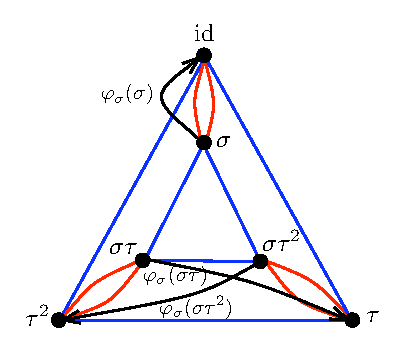
\includegraphics{grugraImages/S3aktion}
\end{center}
$\phi_{\tau}$ ist die Drehung um $120^{\circ}$ im
Uhrzeigersinn. $\phi_{\sigma}$ vertauscht rechts mit links und
innen mit außen.
\end{enumerate}

\PROP Es sei $G$ eine Gruppe, $S\subset G$, und $G_S=\lag S\rag$
bezeichne die von $S$ erzeugte Untergruppe.
\begin{enumerate}
\item Die Zusammenhangskomponenten von $\GR(G,S)$ entsprechen
bijektiv den Linksnebenklassen $g G_S$ für $g\in G$.
\item Es sei $S'\subseteq S$ und $H:=\lag S'\rag \leq G_S$.
Sei $\GR_H(G,S)$ der Graph, der aus $\GR(G,S)$ durch Kontraktion
von $\GR(G,S')$ entsteht.
Dann operiert $G$ auf $\GR_H(G,S)$.
Es ist $E(\GR_H(G,S)) = G/H$ (die Menge der Nebenklassen).
\end{enumerate}
\bew \begin{enumerate}
\item Es bezeichne $\GR_g$ diejenige Zusammenhangskomponente von
$\GR$, die die Ecke $g\in G$ enthält.\\
Die Zusammenhangskomponente $\GR_1$ von $\GR(G,S)$ ist isomorph
zu $\GR(G_S,S)$ (vgl. Bemerkung \ref{bem_GRGS}(1)).
Betrachte $\GR_g$ für beliebiges $g\in G$. Es ist $\phi_g(1)=g$,
also hat $\phi_g(\GR_1)$ nichtleeren Schnitt mit $\GR_g$ und ist
zusammenhängend. Es folgt $\phi_g(\GR_1)=\GR_g$.
Somit ist
\[
E(\GR_g)=(\phi_g)_E(E(\GR_1))=(\phi_g)_E(G_S) = g G_S.
\]
\item
Es ist $K(\GR_H(G,S))=G\times S\backslash S'\times\{-1,1\}$ mit
$\ini(g,s,1)=gH$, $\ter(g,s,1)=gsH$.
Ein Element $g\in G$ operiert wie folgt:
\begin{align*}
g(g'H) &= (gg')H, \\
g(g',s,\eps) &= (gg',s,\eps).
\end{align*}
Aus Teil 1 folgt $E(\GR_H(G,S))=G/H$.
\qed
\end{enumerate}

Wir betrachten nun den Graphen, der aus $\GR$ durch Zusammenfassen
aller Mehrfachkanten entsteht
(wobei die Orientierung jedoch beibehalten wird).

\BEM Sei $\GR$ ein Graph und $\bar{\GR}$ mit
\begin{gather*}
E(\bar{\GR}) = E(\GR), \\
K(\bar{\GR}) =
\{(x,y)\in E(\GR)\times E(\GR) : \exists k\in
	K(\GR):
	\ini(k)=x, \ter(k)=y \},
\end{gather*}
mit $\bar{(x,y)}:=(y,x)$, $\ini(x,y):=x$ und $\ter(x,y):=y$.
\begin{enumerate}
\item Die Abbildung $p:\GR\Ra\bar{\GR}$, $p_E=\id$,
$p_K(k)=(\ini(k),\ter(k))$ ist ein surjektiver Morphismus von
Graphen.
\item Es gibt einen eindeutig bestimmten Gruppenhomomorphismus
$\rho:\Aut(\GR)\Ra\Aut(\bar{\GR})$, so dass für alle
$\gamma\in\Aut(\GR)$ das folgende Diagramm kommutiert:
\[\xymatrix{
\GR \ar[r]^{\gamma} \ar[d]_{p} & \GR \ar[d]^{p} \\
\bar{\GR} \ar[r]_{\rho(\gamma)} & \bar{\GR}
}\]
\item
Es ist
\[
\K{\rho} = \{ \gamma\in\Aut(\GR) : \gamma_E=\id \}.
\]
\end{enumerate}
\textsc{Beweis von 2.:} Definiere $\bar{\gamma}\in\Aut(\bar{\GR})$
durch $\bar{\gamma}_E := \gamma_E$ und
$\bar{\gamma}_K(x,y) := (\ini(\gamma(k)),\ter(\gamma(k)))$
für $(x,y)\in K(\bar{\GR})$, $k\in K(\GR)$ mit $p_K(k)=(x,y)$.
Setze nun $\rho(\gamma):=\bar{\gamma}$.
\qed

\FOLG Es sei $G$ eine Gruppe und $\GR$ ein beliebiger Graph.
\begin{enumerate}
\item Jede Aktion von $G$ auf $\GR$ induziert eine Aktion auf
$\bar{\GR}$.
\item Ist $\GR=\GR(G,S)$ ein Cayley-Graph, so operiert $G$ treu
auf $\GR$ und $\bar{\GR}$.
\item Ist $\GR=\GR_H(G,S)$, so ist die Aktion $\rho$ von $G$ auf
$\bar{\GR}$ genau dann treu, wenn gilt
\[
\BCAP{}{g\in G} gHg^{-1} = \{1\}.
\]
\end{enumerate}
\textsc{Beweis von 3.:} \glqq$\ra$\grqq:
Die Ecken von $\GR$ sind die Linksnebenklassen
$gH$, $g\in G$. Sei $h\in G$ mit $\rho(h)=\id$. Dann ist
$hgH=gH$ für alle $g\in G$, d.h. $g^{-1}hg=h'\in H$.
Folglich ist $h=gh'g^{-1}\in gHg^{-1}$, und da dies für alle
$g\in G$ gilt, ist $h\in \bigcap_{g\in G} gHg^{-1}$.

\glqq$\la$\grqq: Ist $h\in \bigcap_{g\in G} gHg^{-1}$, so ist
$\rho(h)_E=\id_{E(\GR)}=\id_{E(\bar{\GR})}$.
Somit ist $\rho(h)=\id$.
\qed

\SATZ\label{satz_abzb} Es sei $G$ eine abzählbare Gruppe. Dann gibt es einen
zusammenhängenden Graphen $\GR$ mit $\Aut(\GR)\cong G$.

Das folgende Beispiel soll die Idee des anschließenden Beweises
veranschaulichen.
\BSP Betrachte die Kleinsche Vierergruppe\index{Kleinsche Vierergruppe}
$G=\mathrm{V}_4(=\mathrm{D}_2)=\{1,\sigma,\tau,\sigma\tau\}$
mit $S=\{\sigma,\tau\}$.
Es ist
\begin{center}
	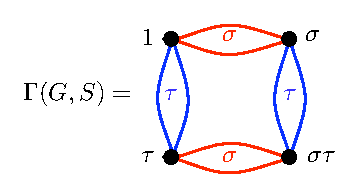
\includegraphics{grugraImages/klein41}
\end{center}
Die Automorphismengruppe dieses Graphen ist aber größer als
$\mathrm{V}_4$. Die Idee ist nun, die $\tau$- bzw. $\sigma$-Kanten
durch \glqq Markierungen\grqq unterscheidbar zu machen,
so dass sie nicht mehr ausgetauscht werden können:
\begin{center}
	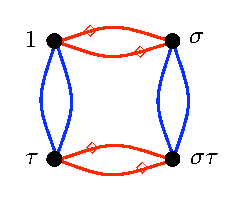
\includegraphics{grugraImages/klein42}
\end{center}
Durch weitere Markierungen wird verhindert, dass Kanten mit ihren
Gegenkanten vertauscht werden:
\begin{center}
	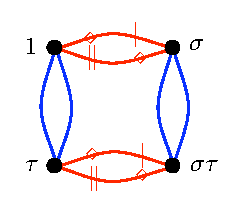
\includegraphics{grugraImages/klein43}
\end{center}

\textsc{Beweis von Satz \ref{satz_abzb}:}
Es sei $S=\{s_1, s_2, \ldots\}$ ein abzählbares Erzeugendensystem
und $\GR_0=\GR(G,S)$.
Für $i\geq 1$ sei $T_i$ der Baum
\begin{center}
	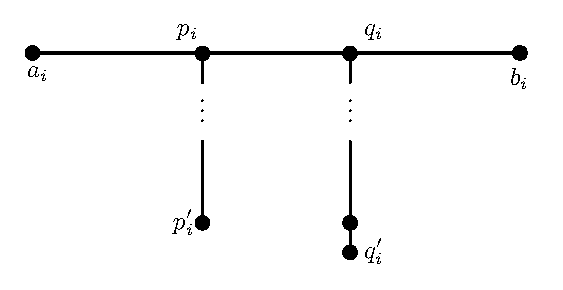
\includegraphics{grugraImages/Ti}
\end{center}
mit $d(p_i,p_i')=2i$ und $d(q_i,q_i')=2i+1$.
Dann ist $T_i\not\cong T_j$ für $i\neq j$ und $\Aut(T_i)=\{\id\}$
für alle $i$. Sei $\GR$ der Graph, der aus $\GR_0$ entsteht, indem
jeder Teilbaum
\begin{center}
	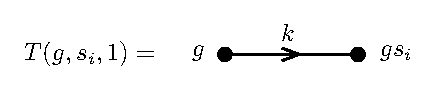
\includegraphics{grugraImages/ggsi}
\end{center}
mit $k=(g,s_i,1)$ durch den Baum $T_i$ ersetzt wird.
Die Abbildung
\[
\GR\Ra\GR_0,\quad T_i\mapsto T(g,s_i,1)
\]
ist ein surjektiver Morphismus.
Nun operiert $G$ auf $\GR$ und jeder Automorphismus von $\GR$
induziert einen Automorphismus von $\GR_0$, der \glqq farbtreu\grqq\
ist.

Ist $\gamma\in\Aut(\GR)$ und $x\in E(\GR)$ mit $\gamma_E(x)=x$,
so ist $\gamma=\id$, denn für $x\not\in E(\GR_0)$ gibt es $i\geq 1$
mit $x\in E(T_i)\backslash\{a_i,b_i\}$.
Dann ist $\gamma|_{T_i}=\id_{T_i}$ und somit ohne Einschränkung
$x\in E(\GR_0)$. Es gibt für jedes $s_i\in S$ genau eine Kante der
Form $(x,s_i,1)$ in $\GR_0$, also in $\GR$ genau einen Baum $T_i$
mit $a_i=x$. Also ist $\gamma=\id$ auf jedem dieser Teilbäume.
Mit Induktion bzw. Anwendung des Zornschen Lemmas folgt, dass
$\gamma$ die Identität ist.

Nun zeigen wir $\Aut(\GR)=G$: Dazu sei $\gamma\in\Aut(\GR)$ und
$g\in E(\GR_0)=G$. Es sei $g':=\gamma_E(g)\in E(\GR_0)=G$
und $h=g'g^{-1}\in G$. Dann ist $\rho(h)_E(g)=hg=g'$.
Es folgt $(\gamma^{-1}\circ\rho(h))_E(g)=g$, also
ist nach dem eben Gezeigten $\gamma^{-1}\circ\rho(h)=\id$ und somit
$\gamma=\rho(h)$.
\qed

% ====================
\section{Quotientengraphen}\label{sec_qg}

\DEF Es sei $\rho:G\Ra\Aut(\GR)$ eine Aktion der Gruppe $G$ auf einem
Graphen $\GR$. Wenn für alle $g\in G$ und alle $h\in K(\GR)$ gilt
\[
\rho(g)_K(k) \neq \bar{k},
\]
so heißt $\rho$ \emph{inversionsfrei}\index{inversionsfreie Aktion}\index{Aktion!inversionsfrei}.

\DB Es sei $\rho:G\Ra\Aut(\GR)$ eine inversionsfreie Aktion.
Dann gibt es einen eindeutig bestimmten
\emph{Quotientengraphen}\index{Quotientengraph}\index{Graph!Quotienten-}
$\GR/G$\index{$\GR/G$ (Quotientengraph)} mit
\begin{align*}
E(\GR/G) &= E(\GR)/G \quad\text{(Menge der Bahnen)},\\
K(\GR/G) &= K(\GR)/G.
\end{align*}
Weiter gelten:
\begin{enumerate}
\item Für $Gk:=\rho(G)_K(k)$\index{$Gk$ (Bahn von $k$)}
ist $\bar{Gk}=G\bar{k}$.
\item Es ist $\ini(Gk)=G \ini(k)$ und $\ter(Gk)=G\ter(k)$.
\item Die kanonische Projektion
	$p:\GR\Ra\GR/G$ ist ein surjektiver Morphismus von Graphen.
\item Ist $f:\GR\Ra\GR'$ ein $G$-invarianter Morphismus von
Graphen (d.h. es ist $f\circ\rho(g)=f$ für alle $g\in G$),
so gibt es genau einen Morphismus
$\bar{f}:\GR/G\Ra \GR'$ mit $f=\bar{f}\circ p$.
\[\xymatrix{
\GR \ar[r]^{f} \ar[d]_{p} & \GR' \\
\GR/G \ar[ru]_{\bar{f}} &
}\]
\end{enumerate}

\BSP Quotientengraphen.
\begin{enumerate}
\item Für $\GR=\GR(\ZZ,\{1\})$ operiert $G=\ZZ$ durch
Translation. Es ist
\begin{center}
	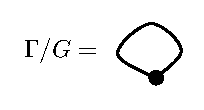
\includegraphics{grugraImages/quot1}
\end{center}
\item Für eine beliebige Gruppe $G$ operiert $G$ auf
$\GR=\GR(G,S)$ durch Linksmultiplikation.
Somit ist
\begin{center}
	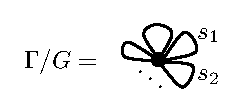
\includegraphics{grugraImages/quot2}
\end{center}
wobei die Anzahl der Schleifen gleich $|S|$ ist.
\item Es sei
\begin{center}
	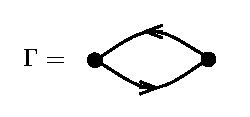
\includegraphics{grugraImages/quot3}
\end{center}
Dann operiert $G=\ZZ/2\ZZ$ auf $\GR$ durch
\begin{itemize}
\item Spiegelung an der horizontalen Achse:
\begin{center}
	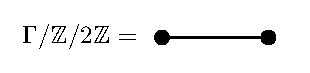
\includegraphics{grugraImages/quot3a}
\end{center}
\item Spiegelung an der vertikalen Achse; in diesem Fall ist
die Operation nicht inversionsfrei.
\item
Drehung um $180^\circ$:
\begin{center}
	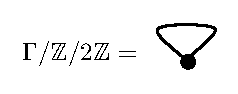
\includegraphics{grugraImages/quot3b}
\end{center}
\end{itemize}
\end{enumerate}

\BEM\label{bem_lift}
Sei $\GR$ ein zusammenhängender Graph und $\rho:G\Ra\Aut(\GR)$
eine inversionsfreie Aktion.
Dann lässt sich jeder Teilbaum von $\GR/G$ nach $\GR$ liften,
d.h. zu einem Teilbaum $T'$ in $\GR/G$ gibt es einen Teilbaum $T$ in
$\GR$, so dass $p|_T:T\Ra T'$ ein Isomorphismus ist.

\bew Es sei
$\calT =\{ T \subset \GR : p|_T \text{ ist injektiv und } p(T)\subseteq T' \}$.
Sofern $\GR\neq\emptyset$, ist auch $\calT\neq\emptyset$.
Außerdem ist $\calT$ durch die Inklusionsrelation partiell geordnet.
Nach dem Zornschen Lemma enthält $\calT$ also ein maximales Element
$T_0$.

Zu zeigen ist nun, dass $p(T_0)=T'$ ist.
Wäre dies nicht der Fall, so können wir in $T'$ eine erste Kante
wählen, die nicht mehr in $p(T_0)$ liegt, genauer gesagt gibt es eine
Kante $k'\in K(T')$ mit $k'\not\in K(p(T_0))$ und
$\ini(k')\in E(p(T_0))$. Dann muss $\ter(k')\not\in E(p(T_0))$ gelten,
denn $p(T_0)$ ist ein Baum, also insbesondere zusammenhängend.
Falls also $\ter(k')\in p(T_0)$ wäre, so gäbe es einen stachelfreien
Weg $w$ in $p(T_0)$ von $\ini(k')$ nach $\ter(k')$.
Dann wäre $(w, \bar{k}')$ ein Kreis in $T'$, im Widerspruch dazu,
dass $T'$ ein Baum ist.\\
Nun sei $\tilde{k}\in p^{-1}(k')$, also
$p(\ini(\tilde{k}))=\ini(k') \in E(p(T_0))$.
Sei $x_0 \in E(T_0)$ die eindeutige Ecke mit $p_E(x_0)=\ini(k')$.
Dann muss es ein $g\in G$ geben mit $g(\ini(\tilde{k}))=x_0$.
Für $k:=g(\tilde{k})$ gilt dann $\ini(k)=x_0$ und $p(k)=k'$.
Somit gilt $k\not\in K(T_0)$ und $\ter(k)\not\in E(T_0)$.
Indem man zu $T_0$ die Kanten $k,\bar{k}$ und die Ecke $\ter(k)$
hinzunimmt, erhält man einen Teilbaum in $\calT$, der $T_0$ als
echten Teilbaum enthält, im Widerspruch zur Maximalität von $T_0$.
Also muss $p(T_0)=T'$ sein.
\qed

\BSP $G=\ZZ/2\ZZ$ operiert auf $\GR$.
\begin{center}
	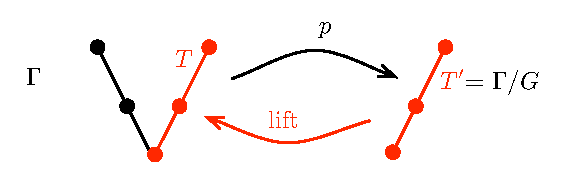
\includegraphics{grugraImages/lift}
\end{center}

Wir betrachten nun den Graphen, der entsteht, indem man jede Kante $k$
eines Graphen $\GR$ durch Einfügen einer weiteren
Ecke unterteilt. Diese neue Ecke kann formal mit der geometrischen
Kante $[k]=\{k,\bar{k}\}$ identifiziert werden.

\DEF Es sei $\GR$ ein Graph. Der Graph $\GRsub$ mit
\begin{align*}
E(\GRsub) &= E(\GR)\cup\{\text{geometrische Kanten von }\GR\} \\
K(\GRsub) &= K(\GR)\times\{-1,1\}
\end{align*}
und
$\ini(k,1)=\ini(k)$, $\ter(k,1)=\ini(k,-1)=[k]$,
$\ter(k,-1)=\ter(k)$ und $\bar{(k, \pm 1)}=(\bar{k},\mp 1)$
heißt \emph{baryzentrische Unterteilung}\index{baryzentrische Unterteilung}\index{Unterteilung}\index{Graph!Unterteilung}\index{Graph!baryzentrische Unterteilung}\index{$\GRsub$ (Unterteilung)}
von $\GR$.
\begin{center}
	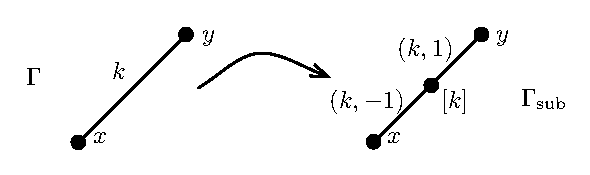
\includegraphics{grugraImages/subdiv}
\end{center}

\BEM Sei $\GR$ ein Graph.
\begin{enumerate}
\item $\GRsub$ hat keine Schleifen.
\item $\GRsub$ ist genau dann zusammenhängend, wenn $\GR$
	zusammenhängend ist.
\item $\GRsub$ ist genau dann ein Baum, wenn $\GR$ ein Baum ist.
\item Ist $\GR$ zusammenhängend, so ist $g(\GR)=g(\GRsub)$.
\end{enumerate}

\BEM Jede Aktion $\rho:G\Ra\Aut(\GR)$ induziert eine inversionsfreie
Aktion $\rhosub:G\Ra\Aut(\GRsub)$.

\bew Definiere $\rhosub$ durch
\[
\rhosub(g)_E(x) :=
\left\{\begin{matrix}
\rho(g)_E(x), & x\in E(\GR) \\
[\rho(g)_K(k)], & x=[k]
\end{matrix}\right.
\]
und
\[
\rhosub(g)_K(k,\eps) :=
(\rho(g)_K(k),\eps),
\quad \eps=\pm 1.
\]
Die Inversionsfreiheit folgt daraus, dass das Vorzeichen von $\eps$
bei der Aktion von $\rho(g)$ erhalten bleibt.
\qed

% =====================
\section{Freie Gruppen}\label{sec_FG}

Definition und erste Eigenschaften einer freien Gruppe $F(X)$
mit Erzeugermenge $X$ findet man in Kapitel I.12 von Lang \cite{lang}.
\index{freie Gruppe}\index{Gruppe!frei}\index{$F(X)$ (freie Gruppe)}
Wir werden davon insbesondere die folgenden benötigen:
\begin{itemize}
\item Für $|X|\geq 2$ ist $F(X)$ nicht abelsch.
\item $F(X)\cong F(Y)$ genau dann, wenn $|X|=|Y|$.
\item Die \emph{universelle Abbildungseigenschaft (UAE)}\index{universelle Abbildungseigenschaft}\index{UAE}
der freien Gruppen besagt, dass es für eine beliebige Gruppe $G$ und
eine Abbildung $f:X\Ra G$ einen eindeutigen Gruppenhomomorphismus
$\phi:F(X)\Ra G$ gibt mit $\phi(x)=f(x)$ für alle $x\in X$.
\end{itemize}

\PROP\label{prop_freibaum}
Es sei $G$ eine Gruppe und $S\subseteq G$. Dann gilt
$G\cong F(S)$ genau dann, wenn $\GR(G,S)$ ein Baum ist.

\bew \glqq$\ra$\grqq:
$\GR(G,S)$ ist zusammenhängend, da $\lag S\rag=G$. Es bleibt zu
zeigen, dass keine Kreise der Länge $\geq 1$ existieren.\\
Es sei $w=(k_1,\ldots,k_n)$ ein Kreis in $\GR(F(S),S)$ mit
$k_i=(g_i,s_i,\eps_i)$.
Es ist $\ter(w)=g_1 s_1^{\eps_1}\cdots s_n^{\eps_n}
=\ini(w)=g_1$, also $s_1^{\eps_1}\cdots s_n^{\eps_n}=1$.
Da $w$ stachelfrei ist, ist $s_1^{\eps_1}\cdots s_n^{\eps_n}$
reduziert und es folgt $n=0$.

\glqq$\la$\grqq:
$S$ erzeugt $G$, da $\GR(G,S)$ zusammenhängend ist.
$S\cap S^{-1}=\emptyset$, da keine Doppelkanten und Schleifen
in $\GR(G,S)$ vorkommen. Wir erhalten einen Gruppenhomomorphismus
$\phi:F(S)\Ra G$ durch $s\mapsto s$.
Dieses $\phi$ ist surjektiv, da $S$ eine Erzeugermenge ist.
Angenommen, $\phi$ sei nicht injektiv. Dann gibt es ein
$s_1^{l_1}\cdots s_n^{l_n} \in \K{\phi}$ mit $n>0$ minimal.
Dann sind $1,s_1^{l_1},\ldots,s_1^{l_1}\cdots s_{n-1}^{l_{n-1}}$
Ecken eines geschlossenen Weges in $\GR(G,S)$, im Widerspruch dazu,
dass $\GR(G,S)$ ein Baum ist. Somit muss $\K{\phi}=\{1\}$ sein
und $\phi$ ist injektiv.
\qed

\BSP Der Cayley-Graph der freien Gruppe mit zwei Erzeugern
$F_2=F(\{x,y\})$.
\begin{center}
	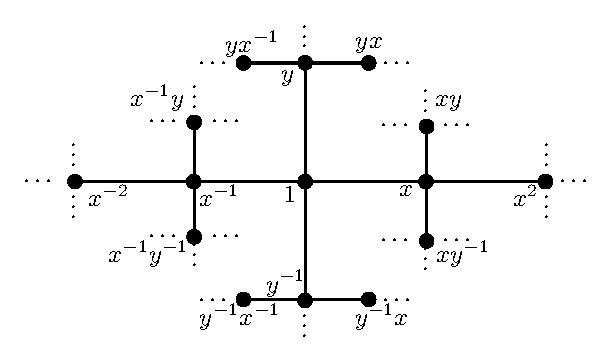
\includegraphics{grugraImages/Fxy}
\end{center}

\DEF $G$ \emph{operiert frei}\index{frei operieren}\index{Aktion!frei}
auf einem Graphen $\GR$, wenn die Aktion sowohl
fixpunktfrei als auch inversionsfrei ist.

\SATZ\label{satz_frei} Eine Gruppe $G$, die frei auf einem Baum
operiert, ist frei.

\bew Es sei $\rho:G\Ra\Aut(\GR)$ eine freie Aktion auf $\GR$,
$\bar{\GR}:=\GR/G$ der Quotientengraph und $\bar{T}$ ein aufspannender
Baum von $\bar{\GR}$. Nach Bemerkung \ref{bem_lift} gibt es einen
Teilbaum $T\subseteq \GR$, der unter der Projektion
$p:\GR\Ra\bar{\GR}$ isomorph auf $\bar{T}$ abgebildet wird.

Es sei $\GR'$ der Graph, der aus $\GR$ durch Kontraktion aller
Teilbäume $gT$, $g\in G$, entsteht.
Für $g\neq 1$ gilt dann $gT\cap T=\emptyset$.
Ist nämlich $x\in E(T)\cap E(gT)$, so ist $x=gx'$ für ein
$x'\in E(T)$. Also ist $p(x)=p(x')$ und da $p|_T$ injektiv ist,
muss $x=x'$ gelten. Da die Aktion aber fixpunktfrei ist, folgt
daraus $g=1$.\\
Nach Proposition \ref{prop_wald} ist $\GR'$ ein Baum. $G$ operiert
inversionfrei auf $\GR'$ und wie gerade gezeigt wurde, ist
die Aktion auch fixpunktfrei.

$\bar{\GR}':=\GR'/G$ hat genau eine Ecke und es ist
$E(\GR')=\{gT:g \in G\}=G$.
Es sei $\tilde{S}:= K(\bar{\GR}')$, setze
$S_0:=\{s\in G: s=\ter(k)\text{ für $k$ mit $\ini(k)=1$ und 
$p(k)\in\tilde{S}$}\}$.
Für $k\in K(\GR')$ mit $\ini(k)=g$, $\ter(k)=g'$ folgt nun,
dass $g^{-1}g'$ in $S_0$ liegt (denn es ist $k=gk'$ mit
$\ini(k')=1$ und $\ter(k')=g^{-1}g'$).
Wähle nun eine Orientierung $\tilde{S}^+\subset\tilde{S}$. Sei $S$
die durch die Orientierung $\tilde{S}^+$ induzierte Teilmenge von $S_0$.\\
Nun überzeugt man sich, dass die Abbildung
$\phi:\GR'\Ra\GR(G,S)$, definiert durch
\begin{align*}
\phi_E(gT) &= g,\\
\phi_K(gT,g'T) &=
\left\{
\begin{matrix}
(g,g^{-1}g',1) & \text{falls } g^{-1}g'\in S \\
\\
(g',g'^{-1}g,-1) & \text{sonst}
\end{matrix}\right.,
\end{align*}
ein Isomorphismus ist.

Mit Proposition \ref{prop_freibaum} folgt $G\cong F(S)$.
\qed

\FOLG\emph{(Satz von Nielsen-Schreier)}\index{Nielsen-Schreier-Satz}\index{Satz!Nielsen-Schreier}\\
Jede Untergruppe einer freien Gruppe ist frei.

\bew
Es sei $G=F(S)$ die freie Gruppe mit Basis $S$ und $H\leq G$ eine
Untergruppe.
Dann ist $\GR=\GR(G,S)$ ein Baum.
$G$ operiert frei auf $\GR$ (das gilt immer für die Aktion einer
Gruppe $G$ auf ihrem Cayley-Graphen $\GR(G,S)$ für jede Teilmenge $S$).
Es folgt, dass $H$ frei auf $\GR$ operiert und nach Satz \ref{satz_frei}
ist $H$ eine freie Gruppe.
\qed

\cleardoublepage
\part{Bass-Serre-Theorie}

% =============
\section{Die Fundamentalgruppe eines Graphen}\label{sec_FG}

\DB Es sei $\GR$ ein zusammenhängender Graph und $p\in E(\GR)$.
\begin{enumerate}
\item $\pi_1(\GR,p)$ sei die Menge der stachelfreien geschlossenen
Wege in $\GR$ mit Anfangs- und Endpunkt $p$.
\item Für $w_1, w_2\in \pi_1(\GR,p)$ sei $w_1\cdot w_2$ der
Weg, den man nach dem Entfernen aller Stachel des aus $w_1$ und $w_2$
zusammengesetzen Weges erhält.
\item Mit dieser Verknüpfung ist $\pi_1(\GR,p)$ eine Gruppe.
Sie heißt \emph{Fundamentalgruppe}\index{Fundamentalgruppe}\index{Gruppe!Fundamental-}\index{$\pi_1(\GR,p)$, $\pi_1(\GR)$ (Fundamentalgruppe)}
von $\GR$ (bzgl. $p$).
\item Für jedes $q\in E(\GR)$ ist $\pi_1(\GR,q)\cong\pi_1(\GR,p)$.
Daher können wir auch $\pi_1(\GR)$ schreiben.
\end{enumerate}
\bew
\begin{itemize}
\item[3.] Das neutrale Element ist der Weg der Länge $0$.
Zu $w=(k_1,\ldots,k_n)$ ist
$\bar{w}=(\bar{k}_n,\ldots,\bar{k}_1)$ invers.

Die Zeichnung veranschaulicht, wie beim Zusammensetzen zweier
stachelfreier Wege neue Stachel autreten können.
\begin{center}
	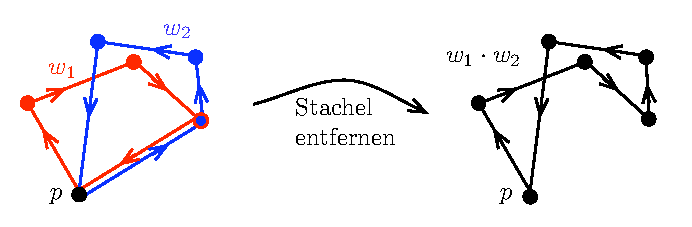
\includegraphics{grugraImages/w1w2}
\end{center}
Hat ein zusammengesetzter Weg $w=(k_1,\ldots,k_n)$ einen Stachel,
so muss $\bar{k}_i=k_{i+1}$ für ein $i$ gelten.
Setze $w^{(1)}:=(k_1,\ldots,k_{i-1},k_{i+2},\ldots,k_n)$ und
wiederholen dieses Vorgehen solange, bis alle Stacheln entfernt sind.
Wir bemerken, dass dies zu einem eindeutigen stachelfreien Weg führt.
Daraus folgt die Wohldefiniertheit der Verknüpfung und ebenso die
Assoziativität.
\item[4.] Es sei $v$ ein Weg in $\GR$ von $p$ nach $q$. Dann ist
\[
\phi:\pi_1(\GR,q)\Ra\pi_1(\GR,p),\quad
w\mapsto vw\bar{v}
\]
ein Gruppenhomorphismus, denn
\[
\phi(w_1 w_2) = v w_1 w_2 \bar{v}
=v w_1 \bar{v} v w_2 \bar{v}
=\phi(w_1)\phi(w_2).
\]
Da es offensichtlich eine Umkehrung gibt, ist $\phi$ bijektiv.
\qed
\end{itemize}

\BSP Fundamentalgruppen.
\begin{enumerate}
\item Ist $\GR$ ein Baum, so ist $\pi_1(\GR,p)=\{1\}$.
\item Es sei
\begin{center}
	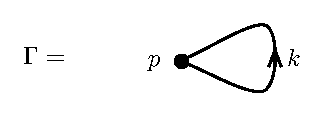
\includegraphics{grugraImages/pi1Z}
\end{center}
Die Gruppe $\pi_1(\GR,p)$ besteht aus dem Weg der Länge $0$
und aus den Wegen, die durch
$n$-faches Durchlaufen von $k$ oder $n$-faches Durchlaufen von
$\bar{k}$ entstehen. Daher ist $\pi_1(\GR,p)\cong\ZZ$.
\item Es sei
\begin{center}
	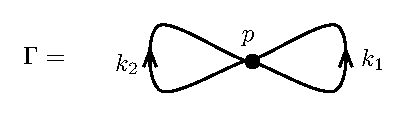
\includegraphics{grugraImages/pi1F2}
\end{center}
In diesem Fall ist $\pi_1(\GR,p)=F_2$.
\end{enumerate}

\PROP\label{prop_zusfrei}
Für jeden zusammenhängende Graphen $\GR$ ist $\pi_1(\GR)$
eine freie Gruppe vom Rang $g(\GR)$.

\bew Für den Fall, dass $\GR$ hat nur eine Ecke hat:\\
Die Kanten $k\in K(\GR)$ können als Elemente von $\pi_1(\GR)$
aufgefasst werden. Für $k\in K(\GR)$ ist $\bar{k}$ das inverse
Element. Die stachelfreien Wege in $\GR$ entsprechen bijektiv
den Kantenfolgen der Form
\[
k_1^{\eps_1},\ldots,k_n^{\eps_n}
\]
mit $n\geq 0$, $\eps_i=\pm 1$ und
$k_{i+1}^{\eps_{i+1}}\neq k_i^{-\eps_i}$.
Diese Stellen aber genau die reduzierten Worte in
$F(K(\GR)^+)$ dar, wobei $K(\GR)^+$ eine Orientierung von
$\GR$ ist.

Nun der Beweis für den allgemeinen Fall:\\
Es sei $T$ ein aufspannender Teilbaum
von $\GR$ und $\GR':=\GR/T$. Nach Bemerkung \ref{bem_GZ}(2) ist
$g(\GR')=g(\GR)$. Zusammen mit dem Fall für eine Ecke genügt es
nun zu zeigen, dass $\pi_1(\GR')\cong\pi_1(\GR)$ ist.
\qed

\BEM Es sei $\GR$ ein zusammenhängender Graph, $Z$ ein zusammenhängender 
Teilgraph $z\in Z$.
Dann gibt es einen surjektiven Homomorphismus
$\phi_Z:\pi_1(\GR,z)\Ra\pi_1(\GR/Z,Z)$, dessen Kern die
normale Hülle von $\pi_1(Z,z)$ ist, d.h.
\[
\K{\phi_Z}=\lag\pi_1(Z,z)\rag_{\mathrm{NT}}:=
\bigcap_{\pi_1(Z,z)\subset N \unlhd \pi_1(\GR,z)} N.
\]
\bew Für $w=(k_1,\ldots,k_n)\in\pi(\GR,z)$ sei
$\psi_Z(w)$ der Weg, der durch Streichen alle Kanten in $K(Z)$
entsteht und $\phi_Z(w)$ der Weg, der durch Entfernen aller Stacheln
aus $\psi_Z(w)$ entsteht. Man sieht leicht, dass $\phi_Z$ ein
Gruppenhomomorphismus ist.

$\phi_Z$ ist surjektiv: Fasse $w$ als Weg in $\pi_1(\GR/Z,Z)$ auf.
Dann sind $k_1,\ldots,k_n\in K(\GR)\backslash K(Z)$.
Ist $\ter(k_i)\neq \ini(k_{i+1})$ in $E(\GR)$, so ist
$\ter(k_i)=\ini(k_{i+1})=Z$ in $E(\GR/Z)$.
Da $Z$ zusammenhängend ist, gibt es einen Weg $v_i$ in $Z$ mit
$\ini(v_i)=\ter(k_i)$ und $\ter(v_i)=\ini(k_{i+1})$.
Also ist
\[
\tilde{w}=
(v_0,k_1,v_1,\ldots,k_n,v_n) \in \pi_1(\GR,z)
\]
ein Weg in $\GR$ mit $\phi_Z(\tilde{w})=w$
(dabei dürfen die Wege $v_i$ die Länge $0$ haben und bei Bedarf
sei $v_0$ ein Weg in $Z$ von $z$ nach $\ini(k_1)$ und $v_n$ ein
Weg in $Z$ von $\ter(k_n)$ nach $z$).
\begin{center}
	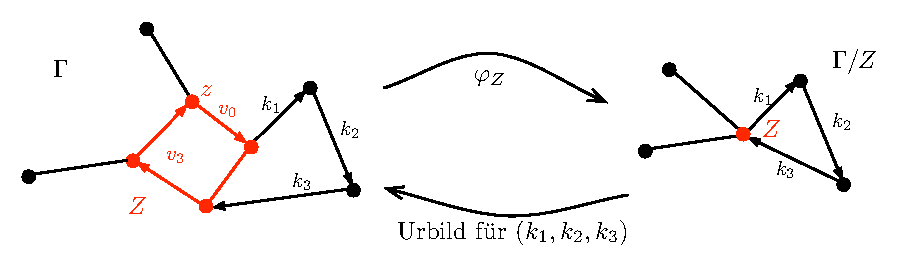
\includegraphics{grugraImages/phiZ}
\end{center}
Offensichtlich liegt $\pi_1(Z,z)$ im Kern von $\phi_Z$. Da der Kern
ein Normalteiler ist, der $\pi_1(Z,z)$ enthält, muss er auch
den Schnitt über alle solchen Normalteiler enthalten,
also $\lag \pi_1(Z,z)\rag_{\mathrm{NT}}\subseteq \K{\phi}$.

Zum Beweis der umgekehrten Inklusionrichtung überlegen wir zuerst,
dass ein Weg $w\in \K{\phi_Z}$ in der Form
\[
v_0 w_1 v_1 w_2 v_2 \cdots w_n v_n
\]
geschrieben werden kann, wobei $v_i$ ein Weg in $Z$ und $w_i$ ein
Weg außerhalb von $Z$ ist (jedoch mit Anfangs und Endpunkt in $Z$).
Es muss $\psi_Z(w)=w_1 w_2 \ldots w_n$ ein Stachel sein.
Wir wählen stachelfreie Wege $u_i$ von $\ter(w_i)$ nach
$z$ und $u_i'$ von $\ter(v_i)$ nach $z$ mit Kanten in $K(Z)$.
Dann können wir $w$ schreiben als
\begin{align*}
w &= v_0 w_1 (u_1 u_1^{-1}) v_1 (u_1' u_1'^{-1}) w_2 \cdots \\
&=\ub{v_0 w_1 u_1}{\in \pi_1(\GR,z)}
\ub{u_1^{-1} v_1 u_1'}{\in \pi_1(Z,z)}
\ub{u_1'^{-1} w_1 u_2}{\in \pi_1(\GR,z)} \cdots .
\end{align*}
Wir können also ohne Einschränkung annehmen, dass
$w_i\in\pi_1(\GR,z)$ und $v_i\in\GR(Z,z)$ gilt. Damit erhalten wir
\begin{align*}
w =&
\ub{w_1 v_1 w_1^{-1}}{\lag \pi_1(Z,z)\rag_{\mathrm{NT}}}
\ub{w_1 w_2 v_2 w_2^{-1} w_1^{-1}}{\lag \pi_1(Z,z)\rag_{\mathrm{NT}}}
\ub{w_1 w_2 w_3 v_3 w_3^{-1} w_2^{-1} w_1^{-1}}{\lag \pi_1(Z,z)\rag_{\mathrm{NT}}}\\
&\cdots
\ub{w_1\cdots w_{n-1}\ldots v_1 w_{n-1}^{-1}\cdots w_1^{-1}}{\lag \pi_1(Z,z)\rag_{\mathrm{NT}}}
\cdot
\ub{w_1\cdots w_n}{\text{Stachel}},
\end{align*}
also $w\in\lag \pi_1(Z,z)\rag_{\mathrm{NT}}$.
\qed

\PROP Zu jedem Graphen $\GR$ gibt es einen Baum $X=X_{\GR}$ und eine
freie Aktion von $\pi_1(\GR)$ auf $X$, so dass
$X/\pi_1(\GR)\cong \GR$.

\bew
Es sei $T$ ein maximaler Teilbaum von $\GR$ und $S$ eine Orientierung
von $K(\GR)\backslash K(T)$. Dann ist $\pi_1(\GR)\cong F(S)$
nach Proposition \ref{prop_zusfrei}.

Die Idee, die der folgenden Konstruktion von $X$ zugrunde liegt,
ist es, für jedes Element von $F(S)$ eine Kopie von
$T$ zu erstellen, so dass $F(S)$ frei auf diesen Kopien operieren
kann. Dazu identifizieren wir ein $s\in S$ mit dem Element
von $\pi(\GR)$, dass $s$ enthält und sonst nur Kanten in $T$
(dies ist eindeutig, da $T$ ein Baum ist).
Nun definieren wir $X$ durch
\begin{align*}
E(X) &:= \BCUP{.}{g\in\pi_1(\GR)} g\cdot E(T), \\
K(X) &:= \Bigl(\BCUP{.}{g\in\pi_1(\GR)} g\cdot K(T)\Bigr)
\cup
\Bigl(\BCUP{}{s\in S}\BCUP{}{g\in\pi_1(\GR)} \{gs, g\bar{s} \}\Bigr)
\end{align*}
mit $\ini(gs):=g\ini(s)$, $\ter(gs):=gs\ter(s)$ und entsprechend
für $g\bar{s}$.
$\pi_1(\GR)$ operiert auf $X$ durch Linksmultiplikation.

Es ist $X/\pi_1(\GR)=\GR$ nach Konstruktion. $X$ ist
zusammenhängend, da $S$ die Gruppe $\pi_1(\GR)$ erzeugt
(vgl. Beweis von Proposition \ref{prop_zusfrei}).
Gäbe es Kreise in $X$, so gäbe es ein reduziertes Wort in den
Elementen aus $S$, im Widerspruch dazu, dass die Aktion frei ist.
Somit muss $X$ ein Baum sein.
\qed

\DEF Der Baum $X_{\GR}$ heißt \emph{universelle Überlagerung}\index{universelle Überlagerung} von $\GR$.

\BSP\label{bsp_univ} Es sei
\begin{center}
	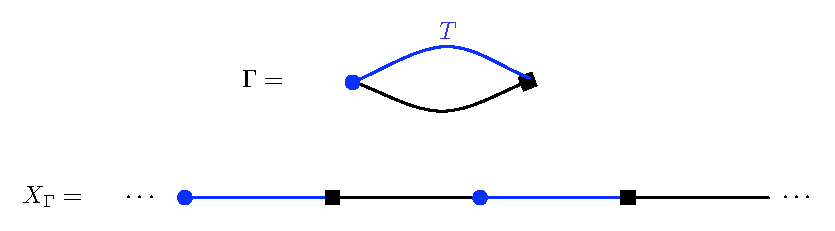
\includegraphics{grugraImages/univ}
\end{center}
$n\in\ZZ=\pi_1(\GR)$ operiert durch Translation um $2n$.

Die hier gegebenen Definitionen der Fundamentalgruppe und der
universellen Überlagerung sind konsistent mit denen aus der
Topologie, wenn wir die Graphen als topologische Teilräume
eines $\RR^n$ auffassen
(vgl. Abschnitte 1.1 und 1.3 in Hatcher \cite{hatcher}).
So entspricht der Graph $\GR$ aus
Beispiel \ref{bsp_univ} dem Einheitskreis $S^1$, dessen
universelle Überlagerung $X_{\GR}$ die reellen Zahlen $\RR$ sind.


% ==================
\section{Freie Produkte und Amalgame}\label{sec_amal}

Es sei $G$ eine Gruppe und $S$ eine Erzeugermenge von $G$.
Die UAE der freien Gruppen impliziert
$G\cong F(S)/\K{\Phi}$ für den Homomorphismus
$\Phi:F(S)\Ra G$, $s\mapsto s$ (man kann sich $\Phi$ als
\glqq Anwendung der in $G$ gültigen Relationen\grqq\ auf Worte
in $F(S)$ vorstellen).\index{Relationen}

\DEF Es sei $R\subset \K{\Phi}$ mit
$\lag R \rag_{\mathrm{NT}} = \K{\Phi}$. Schreibe
\[
\lag S|R \rag := G \cong F(S)/\K{\Phi}.
\]
Dies nennen wir \emph{Präsentation}\index{Präsentation} von $G$
(in Erzeugern und Relationen). Die Präsentation heißt
\emph{endlich}\index{endlich!Präsentation}\index{Präsentation!endlich},
wenn $S$ und $R$ endlich sind. $G$ heißt \emph{endlich präsentierbar}\index{endlich präsentierbar}\index{Gruppe!endlich präsentierbar},
wenn es eine endliche Präsentation von $G$ gibt.

Die Relationen in einer Präsentation werden wir immer multiplikativ
schreiben, auch für Gruppen wie $\ZZ$, die üblicherweise additiv
geschrieben werden.

\BSP Präsentationen.
\begin{enumerate}
\item $F(X) = \lag X | \emptyset\rag$.
\item $\ZZ/3\ZZ = \lag a | a^3=1 \rag$.
\item $\ZZ^2 = \lag a,b | aba^{-1}b^{-1}=1 \rag$.
\end{enumerate}

\BEM Es sei $G=\lag S | R \rag$, $H$ eine weitere Gruppe und
$f:S\Ra H$. Es gelte für alle $r=s_1\cdots s_n\in R$
\[
f(s_1)\cdots f(s_n) = 1.
\]
Dann gibt es genau einen Gruppenhomomorphismus
$\Phi:\lag S|R \rag \Ra H$ mit $\Phi(s)=f(s)$ auf $S$.

\PROP\label{prop_FP}
Es seien $G_1$ und $G_2$ Gruppen. Dann existieren eine Gruppe
$G=G_1*G_2$ und injektive Homomorphismen $\alpha_i:G_i\Ra G$ mit
folgender UAE:\index{UAE}
Sind $H$ eine Gruppe und $\phi_i:G_i\Ra H$ Homomorphismen, so
gibt es einen eindeutigen Homomorphismus $\Phi:G\Ra H$ mit
$\Phi\circ\alpha_i=\phi_i$, d.h. das folgende Diagramm kommutiert:
\[\xymatrix{
G_1 \ar[r]^{\alpha_1} \ar[dr]_{\phi_1} & G_1*G_2 \ar[d]_{\Phi}&
G_2 \ar[l]_{\alpha_2} \ar[dl]^{\phi_2}\\
& H  &
}\]
Wir nennen $G_1*G_2$ das \emph{freie Produkt}\index{freies Produkt}\index{Gruppe!freies Produkt}\index{$G_1*G_2$ (freies Produkt)}
von $G_1$ und $G_2$.

\bew \textsl{Eindeutigkeit}: Es seien $(G, \alpha_i)$ und
$(G',\alpha_i')$ zwei freie Produkte, d.h. sie erfüllen beide die UAE.
Wegen der UAE für $G$ gibt es einen eindeutigen Homomorphismus
$\Phi:G \Ra G'$ mit $\Phi\circ\alpha_i=\alpha_i'$, und wegen der UAE
für $G'$ gibt es einen eindeutigen Homomorphismus
$\Psi:G'\Ra G$ mit $\Psi\circ\alpha_i' = \alpha_i$.
\[\xymatrix{
G \ar[dr]^{\exists_1 \Phi} & \\
G_i \ar[u]^{\alpha_i}\ar[r]_{\alpha_i'} & G'
}\quad
\xymatrix{
G  & \\
G_i \ar[u]^{\alpha_i}\ar[r]_{\alpha_i'} & G'\ar[ul]_{\exists_1 \Psi}
}
\]
Außerdem erfüllt $\id_G:G\Ra G$ die UAE für $G$:
\[\xymatrix{
G \ar[dr]^{\id_G} & \\
G_i \ar[u]^{\alpha_i}\ar[r]_{\alpha_i} & G
}
\]
Aber auch $\Psi\circ\Phi$ erfüllt die UAE, also muss wegen der
Eindeutigkeit $\Psi\circ\Phi=\id_G$ sein und analog
$\Phi\circ\Psi=\id_{G'}$. Somit ist $\Phi$ ein Isomorphismus
von $G$ nach $G'$.

Für die \textsl{Existenz} der Abbildung $\Phi$ betrachten wir zwei
Beweisvarianten.

Variante 1: Schreibe $G_i = \lag S_i|R_i \rag$ und definiere
\[
G := \lag S_1 \os{\cup}{.} S_2 | R_1 \os{\cup}{.} R_2 \rag
\]
(falls notwendig, müssen Elemente umbenannt werden, um eine
disjunkte Vereinigung dieser Mengen zu erhalten).
Die Abbildungen $\alpha_i:G_i\Ra G$, $s\mapsto s$, sind
wohldefinierte Homomorphismen und injektiv.
Zu zeigen ist nun, dass $(G,\alpha_i)$ die UAE erfüllt.
Dazu sei $H$ eine Gruppe und $\phi_i:G_i\Ra H$ Homomorphismen.
Erfüllt $\Phi:G\Ra H$ die UAE (d.h. $\Phi\circ\alpha_i=\phi_i$), so gilt für
alle $s\in S_1\os{\cup}{.} S_2$:
\[
\Phi(s) \us{=}{s\in S_i} \Phi\circ\alpha_i(s)
=\phi_i(s).
\]
Dadurch ist $\Phi$ eindeutig bestimmt.
Umgekehrt ist $\Phi$, gegeben durch die Vorschrift
\[
\Phi(s) := \phi_i(s) \text{ für } s\in S_i, i=1,2,
\]
ein wohldefinierter Gruppenhomomorphismus mit
$\Phi\circ\alpha_i=\phi_i$.

Variante 2: Definiere $G$ durch
\[
G := \{ g_1 h_1 \cdots g_n h_n : g_i\in G_1, h_i \in G_2,
g_2,\ldots,g_n\neq 1, h_1,\ldots,h_{n-1}\neq 1\}.
\]
Mit \glqq Hintereinanderschreiben und Reduzieren\grqq\ als 
Verknüpfung ist $G$ eine Gruppe.
Setze $\alpha_i:G_i\Ra G$, $g\mapsto g$.
Dies sind ein wohldefinierte Homomorphismen, die die UAE erfüllen:
Für eine Gruppe $H$ und Homomorphismen $\phi_i:G_i\Ra H$ ist
ein Homomorphismus $\Phi:G\Ra H$ mit $\Phi\circ\alpha_i=\phi_i$
durch
\begin{align*}
\Phi(g_1 h_1\cdots g_n h_n) &=
\Phi(g_1)\Phi(h_1)\cdots \Phi(g_n)\Phi(h_n) \\
&= \Phi\circ\alpha_1(g_1)\Phi\circ\alpha_2(h_1)\cdots\Phi\circ\alpha_1(g_n)\Phi\circ\alpha_2(h_n) \\
&= \phi(g_1)\phi(h_1)\cdots \phi(g_n)\phi(h_n).
\end{align*}
eindeutig und wohldefiniert.
\qed

\BEM Das direkte Produkt $G_1*G_2$ ist das Koprodukt in der Kategorie
der Gruppen, vgl. Kapitel I.12 in Lang \cite{lang}.\index{Koprodukt}\index{Gruppe!Koprodukt}

\BSP Freie Produkte.
\begin{enumerate}
\item Es ist $F(X)*F(Y) = \lag X|\emptyset\rag*\lag Y|\emptyset\rag
=\lag X\os{\cup}{.} Y|\emptyset\rag$.
Speziell für $\ZZ=F(\{1\})$ ist
$\ZZ*\ZZ=\lag \{1\}\cup\{1'\}|\emptyset\rag=F_2$.
\item Es ist $G*\{1\}=G$.
\item $\ZZ/2\ZZ*\ZZ/2\ZZ=\{1,\sigma\}*\{1,\tau\}
=\{(\sigma)\tau\sigma\tau\cdots\sigma(\tau)\}$.
\item Es ist
\begin{align*}
\ZZ/2\ZZ * \ZZ/3\ZZ &= \{1,\sigma\}*\{1,\tau,\tau^2\} \\
&=\lag\sigma|\sigma^2=1\rag*\lag\tau|\tau^3=1\rag\\
&=\lag\sigma,\tau|\sigma^2=\tau^3=1\rag.
\end{align*}
Dieses freie Produkt ist isomorph zur speziellen projektiven Gruppe\index{projektive Gruppe!spezielle}\index{$\PSL_2$}
\[
\PSL_2(\ZZ)
=\{
A\in \ZZ^{2\times 2} : \det(A)=1
\}/\{-I_2, I_2\}.
\]
Ein Isomorphismus $\Phi$ ist durch das folgende Diagramm gegeben:
\begin{center}
	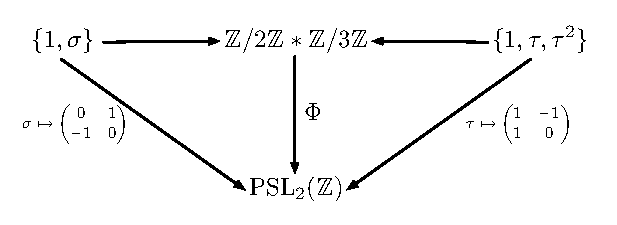
\includegraphics{grugraImages/PSL}
\end{center}
Der Nachweis, dass $\Phi$ in der Tat ein Isomorphismus ist, ist nicht
trivial.
\end{enumerate}

\BEM Die Konstruktion der freien Produkte lässt sich
ohne Weiteres auf beliebige Indexmengen $I$ verallgemeinern:
\begin{enumerate}
\item Es seien $(G_i)_{i\in I}$ Gruppen. Dann gibt es eine (bis auf eindeutige
Isomorphie) eindeutige Gruppe $G=\AST_{i\in I} G_i$ und
Gruppenhomomorphismen $\alpha_i:G_i\Ra G$, so dass
für eine Gruppe $H$ und Homomorphismen $\phi_i:G_i\Ra H$
ein eindeutiger Homomorphismus $\Phi:G\Ra H$ existiert mit
$\Phi\circ\alpha_i=\phi_i$ für alle $i\in I$.
\item Ist $G_i=\lag S_i|R_i\rag$, so ist
$G=\lag \os{\bigcup}{.}_{i\in I}S_i|\os{\bigcup}{.}_{i\in I}R_i \rag$.
\item $G$ ist die Menge aller reduzierten Wörter über
$\os{\bigcup}{.}_{i\in I} G_i$, bei denen aufeinanderfolgende
Buchstaben aus verschiedenen $G_i$ kommen.
\end{enumerate}

\BEM\label{bem_freiprodukt}
Durch die Inklusionen
\begin{align*}
\iota_1:G_1\Ra G_1\times G_2,\quad g\mapsto(g,1) \\
\iota_2:G_2\Ra G_1\times G_2,\quad h\mapsto(1,h)
\end{align*}
ist über die UAE des freien Produktes ein Gruppenhomomorphismus
\[
\rho:G_1*G_2\Ra G_1\times G_2
\]
gegeben. Es gilt:
\begin{enumerate}
\item
\begin{align*}
\rho(g_1 h_1\cdots g_n h_n) &=
\rho(g_1)\rho(h_1)\cdots\rho(g_n)\rho(h_n) \\
&=\rho\circ\alpha_1(g_1)\rho\circ\alpha_2(h_1)\cdots\rho\circ\alpha_1(g_n)\rho\circ\alpha_2(h_n) \\
&=\iota_1(g_1)\iota_2(h_1)\cdots\iota_1(g_n)\iota_2(h_n) \\
&=(g_1,1)(1,h_1)\cdots(g_n,1)(1,h_n) \\
&=(g_1\cdots g_n,h_1\cdots h_n).
\end{align*}
\item $\rho$ ist surjektiv, also
\[
G_1\times G_2 \cong G_1*G_2/\K{\rho}.
\]
\item $\K{\rho}$ ist eine freie Gruppe mit Basis
\[
X=\{ ghg^{-1}h^{-1}:g\in G_1\backslash\{1\},h\in G_2\backslash\{1\}\}.
\]
\end{enumerate}
In Buch von Serre \cite{serre} wird ein elementarer Beweis hierfür
gebracht, den wir nun kurz skizzieren:
Zuerst rechnet man leicht nach, dass $K:=\lag X\rag$ ein Normalteiler
und im Kern von $\rho$ enthalten ist, d.h. es gibt ein $\tilde{\rho}$,
so dass
\[\xymatrix{
G_1*G_2 \ar[r]^{\rho}\ar[d] & G_1\times G_2 \\
G_1*G_2/K \ar[ur]_{\tilde{\rho}}
}\]
kommutiert. Zeigt man nun, dass $\tilde{\rho}$ ein Isomorphismus
(mit Umkehrabbildung $(g,h)\mapsto gh K$) ist, so folgt
$\K{\rho}=K$. Nun muss noch gezeigt werden, dass der Kern frei ist.

Später werden wir einen anderen Beweis für diese Bemerkung geben.

Über die Inklusionen $\iota_1$, $\iota_2$ fassen wir $G_1$ und $G_2$
als Untergruppen von $G_1*G_2$ mit $G_1\cap G_2=\{1\}$ auf.
Dies wollen wir im Folgenden verallgemeinern für Gruppen $G_1$, $G_2$,
$A$ mit $A\leq G_1$ und $A\leq G_2$. Gesucht ist eine Gruppe
$G_1 *_A G_2$ mit $G_1, G_2 \leq G_1 *_A G_2$ und
$G_1 \cap G_2 = A$.

\PROP\label{prop_AP}
Es seien $G_1$, $G_2$, $A$ Gruppen und $\alpha_i:A\Ra G_i$
Homomorphismen.
Dann gibt es eine Gruppe $G_1*_A G_2$ und Homomorphismen
$f_i:G_i\Ra G$ mit $f:=f_1\circ \alpha_1=f_2\circ\alpha_2$,
die folgende UAE erfüllt:
Für alle Gruppen $H$ und Homomorphismen $\phi_i:G_i\Ra H$ mit
$\phi_1\circ\alpha_1=\phi_2\circ\alpha_2$ gibt es genau einen
Homomorphismus $\Phi:G_1 *_A G_2 \Ra H$ mit $\Phi\circ f_i=\phi_i$,
d.h. das folgende Diagramm kommutiert:
\[\xymatrix{
& H & \\
G_1 \ar[r]^{f_1} \ar[ur]^{\phi_1} &
	G_1*_A G_2 \ar[u]_{\Phi} &
	G_2 \ar[l]_{f_2} \ar[ul]_{\phi_2}\\
& A \ar[ul]^{\alpha_1} \ar[ur]_{\alpha_2}  \ar[u]_{f}&
}\]
Wir nennen $G_1*_A G_2$ das \emph{amalgamierte Produkt}\index{amalgamiertes Produkt}\index{$G_1*_A G_2$ (Amalgam)}
von $G_1$ und $G_2$ über $A$.

\bew Die \textsl{Eindeutigkeit} folgt (wie immer bei einer UAE) wie
im Beweis zu Proposition \ref{prop_FP}.

Zur \textsl{Existenz} des amalgamierte Produktes:
Das Diagramm
\[\xymatrix{
G_1 \ar[r]^{\iota_1}  &
	G_1* G_2 &
	G_2 \ar[l]_{\iota_2}\\
& A \ar[ul]^{\alpha_1} \ar[ur]_{\alpha_2}  &
}\]
ist i.A. nicht kommutativ, da
$\iota_1\circ\alpha_1\neq\iota_2\circ\alpha_2$.
Wir entfernen den Teil, der die Kommutativität stört:
\[
N :=
\lag (\iota_1\circ\alpha_1(a))\cdot(\iota_2\circ\alpha_2(a))^{-1}
:a\in A \rag_{\mathrm{NT}}.
\]
Nun kommutiert der obere Teil des Diagramms
\[\xymatrix{
& (G_1*G_2)/N & \\
G_1 \ar[r]^{\iota_1} \ar[ur]^{f_1}  &
	G_1* G_2 \ar[u]_{p} &
	G_2 \ar[l]_{\iota_2} \ar[ul]_{f_2} \\
& A \ar[ul]^{\alpha_1} \ar[ur]_{\alpha_2}  &
}\]
dabei sei $p$ die kanonische Projektion. Definiere nun
\begin{align*}
G_1 *_A G_2 &:= (G_1*G_2)/N \\
f_i &:= p\circ \iota_i, \quad i=1,2.
\end{align*}
Es gilt nun
$f_1\circ\alpha_1(a) = f_2\circ\alpha_2(a)$ für alle $a\in A$,
also
\[
f_1\circ\alpha_1 = f_2\circ\alpha_2.
\]
Es bleibt zu zeigen, dass diese Konstruktion die UAE erfüllt:\\
Es seien $H,\phi_1,\phi_2$ wie gefordert. Wir nutzen die UAE
des freien Produkts, um einen eindeutigen Homomorphismus
$\hat{\Phi}:G_1*G_2\Ra H$ zu erhalten mit
$\hat{\Phi}\circ\iota_i=\phi_i$.
\[\xymatrix{
G_1 \ar[r]^{\iota_1} \ar[dr]_{\phi_1} &
	G_1 * G_2 \ar[d]_{\hat{\Phi}} &
	G_2 \ar[l]_{\iota_2} \ar[dl]^{\phi_2} \\
& H &
}\]
Für alle $a\in A$ gilt
\begin{align*}
\hat{\Phi}((\iota_1\circ\alpha_1(a))\cdot(\iota_2\circ\alpha_2(a))^{-1})
&= (\hat{\Phi}\circ\iota_1\circ\alpha_1(a))
\cdot (\hat{\Phi}\circ\iota_2\circ\alpha_2(a))^{-1} \\
&= (\phi_1\circ\alpha_1(a))\cdot(\phi_2\circ\alpha_2(a))^{-1} \\
&= 1 \qquad\text{(nach Voraussetzung)}
\end{align*}
und somit ist $N$ im Kern von $\hat{\Phi}$ enthalten.
Also gibt es einen eindeutigen Homomorphismus $\Phi$, der das
folgende Diagramm kommutativ macht
\[\xymatrix{
G_1 * G_2 \ar[d]_{p} \ar[r]^{\hat{\Phi}} & H \\
(G_1*G_2)/N \ar[ur]_{\Phi}
}\]
d.h. es ist $\Phi\circ p=\hat{\Phi}$.
Es gilt nun
$\Phi\circ f_i = \Phi\circ p\circ \iota_i=\hat{\Phi}\circ\iota_i
=\phi_i$.
\qed

\BEM Sei $I$ eine beliebige Indexmenge.
Wie beim freien Produkt lässt sich die Definition des
amalgamierten Produktes $\AST_{A,i\in I} G_i$ für Gruppen $A$, $G_i$
und Homomorphismen $\alpha_i:A\Ra G_i$ mit
$i\in I$ übertragen.

\BSP Amalgamierte Produkte.\label{bsp_amprod}
\begin{enumerate}
\item Ist $A=\{1\}$, so ist $G_1*_A G_2=G_1*G_2$.
\item Ist $G_1*_A A=G_1$, so muss wegen der UAE $\alpha_2=\id$ 
gelten.
\item Aus Satz \ref{satz_segment} folgt:
Es ist $\ZZ/4\ZZ *_{\ZZ/2\ZZ} \ZZ/6\ZZ\cong\SL_2(\ZZ)$.
Die Gruppe $\SL_3(\ZZ)$ kann nicht als nichttriviales amalgamiertes
Produkt geschrieben werden.
\item Dieses Beispiel zeigt, dass das amalgamierte Produkt von
den $\alpha_i$ abhängt. Betrachte $\ZZ*_{\ZZ} \ZZ$
mit $\alpha_i=\id$.
Die UAE wird von $\ZZ*_{\ZZ} \ZZ=\ZZ$ erfüllt:
\[\xymatrix{
& \ZZ & \\
\ZZ \ar[ur]^{\id} & & \ZZ \ar[ul]_{\id} \\
& \ZZ \ar[ul]^{\id} \ar[ur]_{\id} &
}\]
Nun betrachte $\ZZ*_{\ZZ}\ZZ$ mit $\alpha_1(z)=2z$ und
$\alpha_2(z)=4z$.
\[\xymatrix{
& \ZZ*_{\ZZ}\ZZ & \\
\ZZ \ar[ur]^{f_1} & & \ZZ \ar[ul]_{f_2} \\
& \ZZ \ar[ul]^{z\mapsto 2z} \ar[ur]_{z\mapsto 4z} &
}\]
Angenommen, es wäre $\ZZ *_{\ZZ}\ZZ=\ZZ$. Dann gibt es
$f_1,f_2:\ZZ\Ra\ZZ$, so dass obiges Diagramm kommutativ ist.
Da $f_2$ als Homomorphismus $\ZZ\Ra\ZZ$ die Form $z\mapsto kz$
haben muss, ist wegen der Kommutativität $f_1$ durch
$z\mapsto 2kz$ gegeben.
Wählt man nun $H=\ZZ/2\ZZ$ und $\phi_1\neq 0$ und $\phi_2=0$,
so gibt es einen eindeutigen Homomorphismus $\Phi:\ZZ\Ra\ZZ/2\ZZ$
mit
\[
\bar{1} = \phi_1(1) = \Phi\circ f_1(1) = \Phi(2k) = \Phi \circ f_2(2)
= \phi_2(2) = \bar{0}.
\]
Dies ist ein Widerspruch.
\item Es sei $G_1=\PSL_2(\QQ)$, $G_2=\ZZ/2\ZZ$ und $A=\ZZ$ und weiter
$\alpha_1:\ZZ\Ra \PSL_2(\QQ)$ ein beliebiger injektiver Homomorphismus
und $\alpha_2:\ZZ\Ra \ZZ/2\ZZ$, $z\mapsto z\mod 2$.
Dann ist
\[
\PSL_2(\QQ)*_{\ZZ} \ZZ/2\ZZ = \{ 0 \}.
\]
\[\xymatrix{
& H & \\
\PSL_2(\QQ) \ar[r]^{f_1} \ar[ur]^{\phi_1} &
	\{0\} \ar[u]_{0} &
	\ZZ/2\ZZ \ar[l]_{f_2} \ar[ul]_{\phi_2}\\
& \ZZ \ar[ul]^{\alpha_1} \ar[ur]_{\alpha_2} &
}\]
Um dies einzusehen, zeigen wir zunächst, dass für Homomorphismen
$\phi_1:\PSL_2(\QQ)\Ra H$ und $\phi_2:\ZZ/2\ZZ\Ra H$ mit
$\phi_1\circ\alpha_1=\phi_2\circ\alpha_2$ stets
$\phi_1=\phi_2=0$ gilt: Da $\alpha_2$ nicht injektiv ist, kann
auch $\phi_2\circ\alpha_2=\phi_1\circ\alpha_1$ nicht injektiv sein.
Da $\alpha_1$ injektiv ist, kann also $\phi_1$ nicht injektiv sein,
also ist $\K{\phi_1}\neq\{I_2\}$.
Da $\PSL_2(\QQ)$ eine einfache Gruppe ist (d.h. sie hat nur
$\{I_2\}$ und $\PSL_2(\QQ)$ selbst als Normalteiler) muss
$\K{\phi_1}=\PSL_2(\QQ)$ gelten, also $\phi_1=0$ und somit
auch $\phi_2\circ\alpha_2=0$. Da $\alpha_2$ surjektiv ist,
folgt $\phi_2=0$.

Die Nullabbildung $\{0\}\Ra H$ erfüllt also die UAE des amalgamierten
Produktes.
\end{enumerate}

Im Folgenden sei $I$ stets eine beliebige Indexmenge und
$G:=\AST_{A,i\in I} G_i$. Außerdem seien alle
$\alpha_i:A\Ra G_i$ injektiv.

\DB\label{bem_NF} \
\begin{enumerate}
\item Es ist
\[
G = \AST_A G_i = (\AST G_i)/N
=\bigl\{x_1\cdots x_n : n\in\NN, x_j\in\BCUP{.}{i\in I} G_i \bigr\}.
\]
Diese Darstellung der Elemente ist i.A. nicht eindeutig.
Ist etwa $a\in A$, $g\in G_i$ und $h\in G_j$ mit $i\neq j$, so
ist stets
\[
(ga)hN = g(ah)N.
\]
\item Für jedes $i$ ist $A\leq G_i$. Es gibt also ein Vertretersystem
$S_i$ der Rechtsnebenklassen von $A$ in $G_i$, so
dass für jede Rechtsnebenklasse genau ein Repräsentant
in $S_i$ enthalten ist und $A$ selbst durch $1$ in $S_i$ repräsentiert
wird.
Dann kann jedes Element $x\in G$ eindeutig geschrieben werden
als
\[
x = as_1\cdots s_n N
\]
mit $a\in A$, $n\in\NN$ und $s_{\nu}\in S_{i_{\nu}}\backslash\{1\}$,
$i_{\nu}\neq i_{\nu+1}$.
Wir bezeichnen diese Darstellung als \emph{Normalform}\index{Normalform} von $x$.
\end{enumerate}
\textsc{Beweis von 2.:}
Setze
\[
X :=
\{ (a,s_1,\ldots,s_n): a\in A, n\in\NN,
s_{\nu}\in S_{i_{\nu}}\backslash\{1\},
i_{\nu}\neq i_{\nu+1} \}
\]
und
\[
\beta:X\Ra G,\quad (a,s_1,\ldots,s_n)\mapsto a s_1\cdots s_n N.
\]
$\beta$ ist offensichtlich surjektiv. Zu zeigen bleibt,
dass $\beta$ auch injektiv ist:\\
Setze
\[
Y_i :=
\{ (a,s_1,\ldots,s_n)\in X : a=1, s_1\not\in S_i \}.
\]
Dann ist die Abbildung
\[
X\Ra A\times S_i\times Y_i,\quad
(a,s_1,\ldots,s_n)\mapsto \left\{
\begin{matrix}
(a,s_i,(1,s_2,\ldots,s_n)), & s_1\in S_i \\
(a,1,(1,s_1,\ldots,s_n)), & s_1\not\in S_i
\end{matrix}
\right.
\]
bijektiv mit Umkehrung
\[
A\times S_i\times Y_i \Ra X,\quad
(a,s,(1,s_1,\ldots,s_n))\mapsto \left\{
\begin{matrix}
(a,s,s_1,\ldots,s_n), & s \neq 1 \\
(a,s_1,\ldots,s_n), & s = 1
\end{matrix}
\right..
\]
Da es auch eine Bijektion
$A\times S_i \Ra G_i$, $(a,s)\mapsto as$, gibt,
erhalten wir eine Bijektion
$\theta_i:X\Ra G_i\times Y_i$.
Da $G_i$ auf $G_i\times Y_i$ durch $g(g',y):=(gg',y)$ operiert,
induziert $\theta_i$ eine Aktion von $G_i$ auf $X$.
Wir erhalten für $a\in A\leq G_i$
\[
a(b,s_1,\ldots,s_n) = (ab,s_1,\ldots,s_n)\qquad (*)
\]
und für $s\in S_i\backslash\{1\}$, $x=(1,s_1,\ldots,s_n)\in X$ mit
$s_1\not\in S_i$
\[
s(1,s_1,\ldots,s_n) = (1,s,s_1,\ldots,s_n). \qquad (**)
\]
Nach $(*)$ ist die Aktion von $A$ auf $X$ unabhängig von der Wahl
der Einbettung in $G_i$. Daher liefert die UAE von $G$ eine
Operation von $G$ auf $X$ durch
\[
(x_1\cdots x_n N)\cdot x := x_1\cdots x_n x,\qquad x\in X, x_i\in G_i.
\]
Es sei $\alpha:G\Ra X$, $g\mapsto g (1)$.
Damit gilt für alle $(a,s_1,\ldots,s_n)\in X$:
\begin{align*}
\alpha\circ\beta(a,s_1,\ldots,s_n)
&= \alpha(a s_1\cdots s_n N) = a s_1\cdots s_n (1) \\
&\os{=}{(**)} a s_1\cdots s_{n-1}(1,s_n) \\
&\os{=}{(**)} \ldots \\
&\os{=}{(**)} a(1,s_1,\ldots,s_n) \\
&\os{=}{(*)} (a,s_1,\ldots,s_n).
\end{align*}
Folglich ist $\alpha\circ\beta=\id$ und $\beta$ injektiv.
\qed

\FOLG\
\begin{enumerate}
\item Sind $\alpha_1$ und $\alpha_2$ injektiv, so sind auch
$f_1$, $f_2$ und $f$ injektiv.
\item In $\AST_{A} G_i$ gilt $\BCAP{}{i\in I} G_i = A$.
\end{enumerate}
\bew
\begin{enumerate}
\item Wähle $g,g'\in G_1$ mit $f_1(g)=f_1(g')$.
Dann haben wir eindeutige Darstellungen $g=as$ und $g'=a's'$
und somit $gN=g'N$. Es folgt und $asN=a's'N$ und wegen der
Eindeutigkeit $a=a'$ und $s=s'$.
\item Angenommen es gibt ein $x\in \bigcap G_i$, $x\not\in A$.
Dann gibt es für alle $i$ eine eindeutige Darstellung
$x=a_i s_i$ mit $s_i\neq 1$.
Es folgt $xN=a_i s_i N$ für alle $i$.
Da alle $a_i$ gleich sein müssen, müssen auch alle $s_i$ gleich sein
und somit aus demselben $S_i$ stammen, im Widerspruch zur Annahme.
\qed
\end{enumerate}

Im Folgenden werden wir einfach $x_1\cdots x_n$ für
$x_1\cdots x_n N$ schreiben.

\DB\ \begin{enumerate}
\item Es sei $x=a s_1\cdots s_n \in G=\AST_A G_i$ in Normalform.
$\typ(x):=(i_1,\ldots,i_n)$ heißt \emph{Typ}\index{Typ}\index{$\typ(x)$}
von $x$ und
$\ell(x):=n$ die \emph{Länge}\index{Länge}\index{$\ell(x)$ (Länge)} von $x$.
Typ und Länge sind unabhängig vom Vertretersystem.
\item Es ist $\ell(x)=0$ genau dann, wenn $x\in A$.
\item Es ist $\ell(x)\leq 1$ genau dann, wenn $x\in G_i$ für
ein $i$.
\item Es sei $\ell(x)\geq 2$. Dann heißt $x$ \emph{zyklisch reduziert}\index{zyklisch reduziert},
wenn $i_1\neq i_n$.
\item Jedes $x\in G$ ist konjugiert zu einem zyklisch reduzierten
Element oder zu einem Element, dass bereits in einem $G_i$ enthalten
ist.
\item Jedes zyklisch reduzierte Element hat unendliche Ordnung.
\item Jedes $x\in G$ von endlicher Ordnung ist konjugiert zu
einem Element aus einem der $G_i$.
\item Sind alle $G_i$ torsionsfrei (d.h. sie enthalten keine Elemente
endlicher Ordnung), so ist auch $G$ torsionsfrei.
\end{enumerate}
\bew 7. und 8. folgen direkt aus 5. und 6. .
\begin{enumerate}
\item[5.] Es sei $n\geq 2$ und $x$ nicht zyklisch reduziert.
Es ist
\begin{align*}
s_n x s_n^{-1}
&= \ub{s_n a s_1}{\in G_{i_1}} s_2\cdots s_{n-1} \\
&= a's' s_2\cdots s_{n-1}
\end{align*}
mit geeigneten $a'\in A$, $s'\in S_{i_1}$.
Es ist $\ell(a's's_2\cdots s_{n-1})<\ell(x)$.
Mit Induktion folgt die Behauptung.
\item[6.] Es sei $x=a s_1\cdots s_n$ in Normalform mit $\ell(x)\geq 2$
und $i_1\neq i_n$.
Wiederholtes bilden der Normalform liefert:
\begin{align*}
x^2 &= a s_1 \cdots \ub{s_n a}{=a' s_n'} s_1 \cdots s_n \\
&= a s_1 \cdots \ub{s_{n-1} a'}{=a'' s_{n-1}'} s_n' s_1\cdots s_n \\
&= \ldots\\
&= \tilde{a} s_1' \cdots s_n' s_1 \cdots s_n
\end{align*}
für geeignete $\tilde{a},a',a'',\ldots\in A$ und
$s_{\nu}'\in S_{i_{\nu}}$.
Der letzte Ausdruck ist die Normalform von $x^2$, da $s_n'$ und $s_1$
aus verschiedenen $S_{i_{\nu}}$ stammen.
Es folgt nun $\ell(x^2)=2\ell(x)$,
$\typ(x^2)=(i_1,\ldots,i_n,i_1,\ldots,i_n)$.
Induktiv erhalten wir $\ell(x^k)=k\ell(x)$,
also $x^k\neq 1$ für alle $k\geq 1$.
\qed
\end{enumerate}

%======================
\section{Graphen von Gruppen}\label{sec_GvG}

\DB Es sei $G$ eine Gruppe, $\GR$ ein Graph und
$\rho:G\Ra\Aut(\GR)$ eine Aktion von $G$ auf $\GR$.
Wir schreiben $gx:=\rho(g)_E(x)$ und $gk:=\rho(g)_K(k)$.
\begin{enumerate}
\item Für $x\in E(\GR)$ sei
\[
G_x := \{ g\in G : gx = x \}
\]
die \emph{Fixgruppe}\index{Fixgruppe}\index{Gruppe!Fix-}\index{$G_x$ (Fixgruppe)}\index{Stabilisator (siehe Fixgruppe)}
von $x$.
Entsprechend ist $G_k$ für $k\in K(\GR)$ definiert.
\item Für alle $g\in G$ und $x\in E(\GR)$ gilt
\[
G_{gx} = g G_x g^{-1},
\]
und enstprechendes für $G_{gk}$, $k\in K(\GR)$.
\item Für jede Kante $k\in K(\GR)$ gilt
\[
G_k \leq G_{\ini(k)}\cap G_{\ter(k)}.
\]
\end{enumerate}
\bew \begin{enumerate}
\item[2.] Es ist $h(gx)=gx$ genau dann, wenn $(g^{-1} h g)x=x$ gilt.
Es ist also $h\in G_{gx}$ genau dann, wenn $g^{-1}hg\in G_x$ gilt,
und dies ist wiederum äquivlent zu $h\in gG_x g^{-1}$.
\item[3.] Klar.
\qed
\end{enumerate}

\PROP Jede inversionsfreie Aktion $\rho:G\Ra\Aut(\GR)$ bestimmt
folgende Daten:
\begin{itemize}
\item Einen Graphen $\bar{\GR}:= \GR/G$.
\item Für jede Ecke $x\in E(\bar{\GR})$ eine Gruppe $G_x$, nämlich
$G_x := G_{\tilde{x}}$ für ein Urbild $\tilde{x}\in E(\GR)$ von $x$.
\item Für jede Kante $k\in K(\bar{\GR})$ eine Gruppe $G_k$, nämlich
$G_k := G_{\tilde{k}}$ für ein Urbild $\tilde{k}\in K(\GR)$ von $k$.
Dabei ist $G_{\bar{k}}=G_k$ für die Gegenkante $\bar{k}$.
\item Für jede Kante $k$ einen injektiven Gruppenhomomorphismus
$\alpha_k:G_k\Ra G_{\ini(k)}$
(durch $G_{\tilde{k}}\hookrightarrow G_{\ini(\tilde{k})}$).
Beachte: $\alpha_{\bar{k}}:G_k\Ra G_{\ter(k)}$.
\end{itemize}
Ein solches Tupel
\[
\GG(\bar{\GR}):=\GG(\GR,\rho):=
(\bar{\GR},\
(G_x)_{x\in E(\bar{\GR})},\
(G_k)_{k\in K(\bar{\GR})},\
(\alpha_k)_{k\in K(\bar{\GR})})
\]
heißt
\emph{Graph von Gruppen}\index{Graph!von Gruppen}\index{$\GG(\GR,\rho)$ (Graph von Gruppen)}. Wir verwenden auch die Kurzform
$\GG=(\bar{\GR}, G_x, G_k, \alpha_k)$.

\BSP Graphen von Gruppen.
\begin{enumerate}
\item Ist $\rho$ eine freie Aktion, so ist $G_x=G_k=\{1\}$ für
alle $x\in E$, $k\in K$.
\item Es sei $\GR$ die unendliche lineare Kette
\begin{center}
	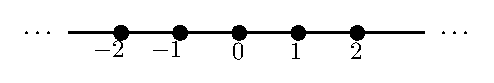
\includegraphics{grugraImages/cay1}
\end{center}
und $G=\Aut(\GR)$ wird erzeugt von der Translation $t$ um $1$ und
der Spiegelung $s$ an der $0$. Die Aktion von $G$ auf $\GR$ ist nicht
inversionsfrei. $G$ operiert jedoch inversionsfrei auf
der baryzentrischen Unterteilung
\begin{center}
	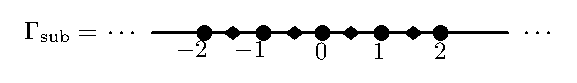
\includegraphics{grugraImages/cay1sub}
\end{center}
Es ist
\begin{center}
	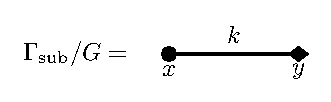
\includegraphics{grugraImages/cay1subquot}
\end{center}
und $G_x=\ZZ/2\ZZ$, $G_y=\ZZ/2\ZZ$, $G_k=\{1\}$.
Der entsprechende Graph von Gruppen ist
\begin{center}
	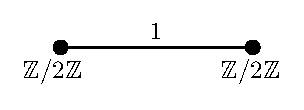
\includegraphics{grugraImages/GvG1}
\end{center}
Wir werden später sehen, dass $G\cong \ZZ/2\ZZ*\ZZ/2\ZZ$ gilt.
\item $G=\SL_2(\ZZ)$ wird erzeugt von
\[
T=\begin{pmatrix}
1 & 1 \\ 0 & 1
\end{pmatrix},\quad
S=\begin{pmatrix}
0 & -1 \\ 1 & 0
\end{pmatrix}.
\]
Es ist $\ord(T)=\infty$ und $\ord(S)=4$.
Die Gruppe $\SL_2(\ZZ)$ operiert auf der komplexen oberen Halbebene\index{obere Halbebene}\index{Halbebene}
\[
\hh = \{ z\in\CC : \Im(z) > 0 \}.
\]
Die Aktion ist für
$A=\begin{pmatrix} a&b \\ c&d \end{pmatrix}\in \SL_2(\ZZ)$
und $z\in \hh$ definiert durch die \emph{Möbiustransformation}\index{Möbiustransformation}
\[
A\cdot z := \frac{az+b}{cz+d},
\]
insbesondere gilt $T\cdot z= z+1$ und $S\cdot z=-\frac{1}{z}$.
Wir betrachten nun zunächst den \emph{Fundamentalbereich}\index{Fundamentalbereich}
\[
F = \Bigl\{ z\in \hh : -\frac{1}{2}\leq \Re(z) \leq \frac{1}{2},
|z| \geq 1 \Bigr\}
\]
in $\hh$.
\begin{center}
	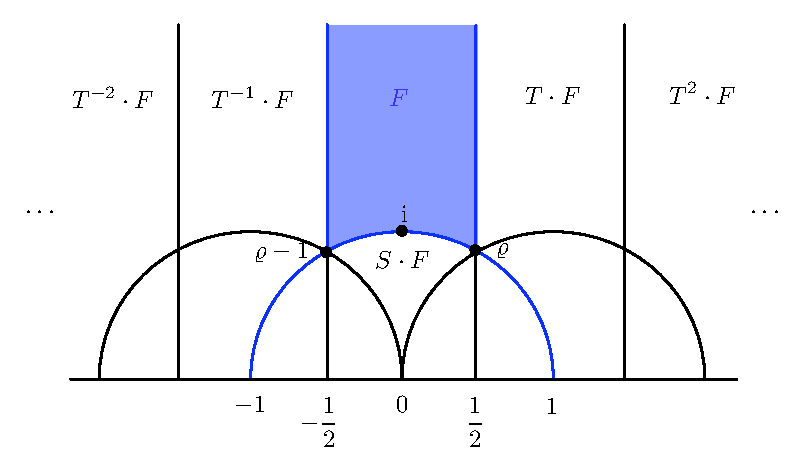
\includegraphics{grugraImages/fundbereich}
\end{center}
Alle $z\in \hh$ können durch wiederholte Aktion von $T$ und $S$
in den Fundamentalbereich $F$ bewegt werden.
Es bezeichne $R_{\rho}$ das Kreissegment, das von
$\rho$ durch $\i$ nach $\rho-1$ läuft:
\begin{center}
	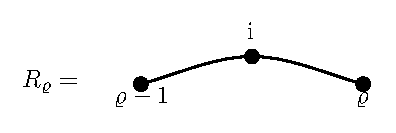
\includegraphics{grugraImages/rho}
\end{center}
$\SL_2(\ZZ)$ operiert auf dem Baum
\[
\GR := \BCUP{}{A\in\SL_2(\ZZ)} A\cdot R_{\rho}.
\]
Den Baum kann man durch wiederholte Operation von $T$ und $S$
auf $R_{\rho}$ Schritt für Schritt aufbauen.
\begin{center}
	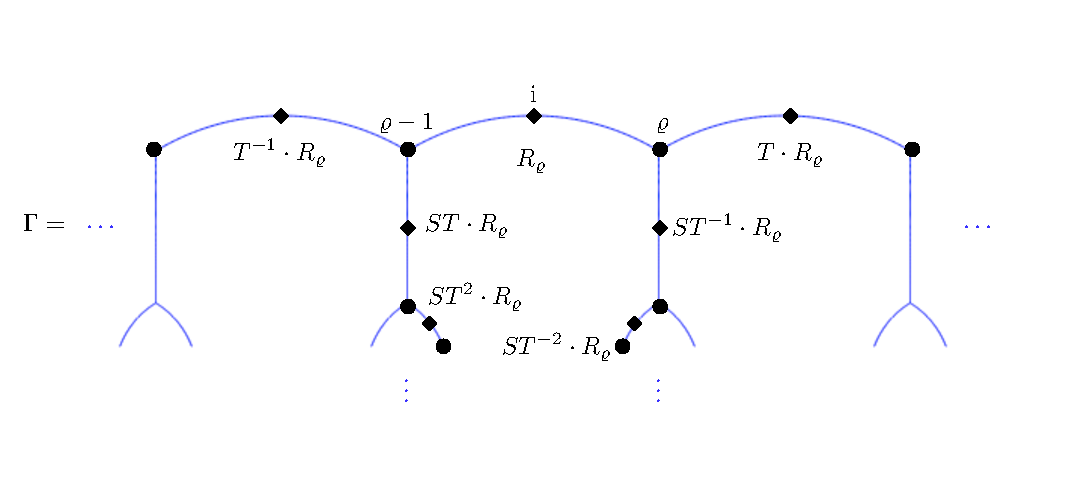
\includegraphics[width=15cm]{grugraImages/Hbaum}
\end{center}
Der Quotientengraph ist
\begin{center}
	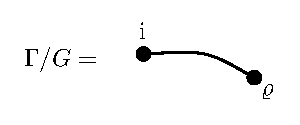
\includegraphics{grugraImages/rhoquot}
\end{center}
Es ist $G_{\i}=\lag S\rag \cong \ZZ/4\ZZ$,
$G_{\rho}=\lag TS\rag\cong \ZZ/6\ZZ$ und
$G_k=\lag I_2\rag \cong\ZZ/2\ZZ$.
Die Abbildung $\alpha_k$ ist durch $\alpha_k(-I_2)=S^2$ und
$\alpha_{\bar{k}}$ durch
$\alpha_{\bar{k}}(-I_2)=(TS)^3$ gegeben.
Aus Teil 1 von Satz \ref{satz_segment} wird folgen,
dass $\SL_2(\ZZ)\cong \ZZ/4\ZZ*_{\ZZ/2\ZZ} \ZZ/6\ZZ$ ist.

Mit Hilfe der hyperbolischen Geometrie lässt sich zeigen, dass
$\GR$ ein Baum ist:\\
Man fasst die Halbebene $\hh$ als hyperbolischen Raum auf, in dem
die Geraden (genauer: die Geodätischen) die Halbkreise und Halbgeraden
sind, die senkrecht auf der reellen Achse stehen (es gibt zwar
zu je zwei Punkten genau eine Gerade durch diese Punkte, aber
das Parallelenaxiom ist nicht erfüllt).
Versieht man $\hh$ mit der hyperbolischen Metrik
$\d s^2 = \frac{1}{y}(\d x^2 + \d y^2)$, so ist die kürzeste
Verbindung zwischen zwei Punkten durch eine solche Gerade gegeben.
Die Elemente von $\SL_2(\RR)$ (also insbesondere $S$ und $T$) sind
Isometrien bzgl. dieser Metrik. Mit Hilfe der Metrik kann man nun
zeigen, dass Abstände beim Entlangwandern von $\GR$ immer größer
werden und es somit keine Kreise geben kann.
\end{enumerate}

% =============
\section{Segmente und Amalgame}\label{sec_seg}

Wir schreiben im Folgenden $(x,y;k)$ für ein Segment\index{Segment}
der Form
\begin{center}
	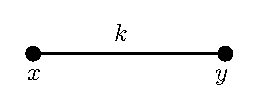
\includegraphics{grugraImages/segment}
\end{center}

\DB Es sei $\rho:G\Ra\Aut(\GR)$ eine inversionsfreie Aktion von $G$
auf $\GR$.
\begin{enumerate}
\item Ein Teilgraph $T$ von $\GR$ heißt \emph{Fundamentalbereich}\index{Fundamentalbereich}
von $\GR$ für $\rho$, wenn die Einschränkung
$p|_T : T \Ra \GR/G$
der kanonischen Projektion ein Isomorphismus ist.
\item Ist $\GR$ ein Baum, so existiert ein Fundamentalbereich genau
dann, wenn $\GR/G$ ein Baum ist.
\end{enumerate}
\textsc{Beweis von 2.:} \glqq$\ra$\grqq: Ist $\GR$ zusammenhängend,
so ist auch $\GR/G$ zusammenhängend. Es folgt, dass $T$ 
zusammenhängend und somit ein Teilbaum in $\GR$ ist.
Aus $T\cong \GR/G$ folgt, dass $\GR/G$ ein Baum ist.

\glqq$\la$\grqq: Jeder Teilbaum von $\GR/G$ lässt sich nach
Bemerkung \ref{bem_lift} liften.
\qed

\SATZ \label{satz_segment}
Es sei $\GR=(x,y;k)$ ein Segment und
$\GG=(\GR,G_x,G_y,G_k,\alpha_k,\alpha_{\bar{k}})$
ein Graph von Gruppen über $\GR$.
Weiter sei $G:=G_x *_{G_k} G_y$.
\begin{enumerate}
\item Es sei $H$ eine Gruppe, $\Xi$ ein Graph,
$\rho:H\Ra\Aut(\Xi)$ eine inversionsfreie Aktion
mit $\Xi/H\cong\GG$ und das Segment $T=(p,q;l)$ ein
Fundamentalbereich von $\Xi$.
Die Abbildungen
$G_x \os{\Ra}{\sim} H_p \hookrightarrow H$ und
$G_y \os{\Ra}{\sim} H_q \hookrightarrow H$
induzieren einen Homomorphismus
$\phi:G \Ra H$. Es ist $\Xi$ genau dann ein Baum, wenn
$\phi$ ein Isomorphismus ist.
\item Es gibt einen (bis auf Isomorphie eindeutigen) Baum $\Xi$ 
und eine Aktion $\rho:G\Ra\Aut(\Xi)$, so dass
$\Xi/G\cong\GG$ ist.
\end{enumerate}
\bew \begin{enumerate}
\item Dieser Teil des Satzes folgt sofort, wenn die folgenden
Teilbehauptungen bewiesen sind.
\begin{enumerate}
\item Zeige: $\Xi$ ist zusammenhängend genau dann, wenn $\phi$
surjektiv ist, was genau dann der Fall ist, wenn
$H$ von $H_p$ und $H_q$ erzeugt wird.\\
Es sei $\Xi'$ die Zusammenhangskomponente von $\Xi$, die $T$ enthält.
Weiter sei $H'=\{ h\in H : h\Xi' = \Xi' \}$.
Es gilt: $\Xi$ ist zusammenhängend genau dann, wenn $\Xi'=\Xi$, was
genau dann der Fall ist, wenn $H'=H$ ist.
Es genügt also zu zeigen:
\[
H' = H'' := \lag H_p \cup H_q \rag.
\]
\glqq$\supseteq$\grqq:
Sei $h\in H_p\cup H_q$. Dann ist
$hT\cap T\neq\emptyset$ und somit $hT\cup T$ zusammenhängend.
Es folgt $h\Xi'=\Xi'$, also $h\in H'$.\\
\glqq$\subseteq$\grqq:
Es ist $H'' T\cup(H\backslash H'')T= \Xi$. Außerdem ist
$H'' T\cap(H\backslash H'')T = \emptyset$, denn wäre
$h''p=hp$ mit $h''\in H''$ und $h\in H\backslash H''$
wäre $h^{-1}h''p=p$, also $h^{-1}h''\in H_p\leq H''$ und folglich
$h\in H''$, im Widerspruch zur Wahl von $h$.
Somit ist $\Xi'\subset H'' T$. Für $h\in H'$ ist
$hT\subseteq h\Xi'=\Xi'\subseteq H'' T$, also $h\in H''$.
\item Zeige: $\Xi$ enthält keine Kreise genau dann, wenn
$\phi$ injektiv ist.\\
Es sei $w=(k_1,\ldots,k_n)$ ein stachelfreier Weg in $\Xi$.
Dann gilt:
\begin{itemize}
\item Für alle $i=1,\ldots,n$ gibt es ein $h_i\in H$ mit
$k_i=h_i\cdot l_i$, wobei $l_i = l$ oder $l_i = \bar{l}$.
\item Es ist $l_{i+1}=\bar{l}_i$.
\item Es ist $h_{i+1}=h_i g_i$ für ein
$g_i\in H_{\ter(l_i)}=H_{\ini(l_{i+1})}$.
\begin{center}
	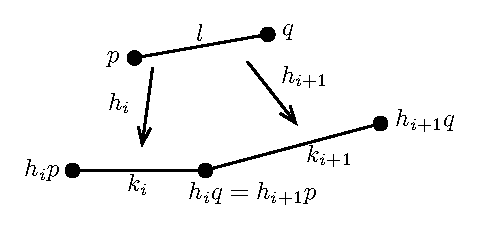
\includegraphics{grugraImages/pql}
\end{center}
Es ist nämlich (mit $p_i:=\ter(l_i)$)
\begin{align*}
h_{i+1} p_i &= h_{i+1} \ini(l_{i+1}) = \ini(h_{i+1} l_{i+1}) 
= \ini(k_{i+1}) \\
&= \ter(k_i) = \ter(h_i l_i) = h_i \ter(l_i) \\
&= h_i p_i,
\end{align*}
also $h_i^{-1} h_{i+1} \in H_{p_i}$.
\item Da $w$ stachelfrei ist, gilt $g_i\not\in H_l$.
\item $w$ ist geschlossen genau dann, wenn $\ter(k_n)=\ini(k_1)$,
was genau dann der Fall ist, wenn
\[
h_1 \ini(l_1) = h_n \ini(l_1)
= h_1 g_1\cdots g_{n-1} \ini(l_1)
\]
ist. Es ist $g_1\cdots g_{n-1}\in H_{\ini(l_1)}\subset H_p\cup H_q$.
Aber $g_1\cdots g_{n-1}$ liegt als Element von
$G=G_x *_{G_k} G_y\cong H_p *_{H_l} H_q$ nicht in $H_p$ oder $H_q$.
Es folgt, dass $\Xi$ genau dann einen Kreis enthält, wenn
$\phi$ nicht injektiv ist.
\end{itemize}
\end{enumerate}
\item Definiere $\Xi$ durch
\begin{align*}
E(\Xi) &:= G/G_x \cup G/G_y, \\
K(\Xi) &:= G/G_k \cup \bar{G/G_k}, \\
\ini(g G_k) &:= g G_x,\ \ter(g G_k):= g G_y.
\end{align*}
$\Xi$ ist ein Graph. $G$ operiert durch Linksmultiplikation auf
$\Xi$, und das Segment $(1\cdot G_x, 1\cdot G_y;1\cdot G_k)$
ist ein Fundamentalbereich dieser Aktion.
Nach Teil 1 ist $\Xi$ ein Baum.
\qed
\end{enumerate}

\FOLG Aus Teil 1 von Satz \ref{satz_segment} folgt
\[
\SL_2(\ZZ) \cong \ZZ/4\ZZ *_{\ZZ/2\ZZ} \ZZ/6\ZZ.
\]

\FOLG\label{folg_H_frei}
Es sei $G=G_1 *_A G_2$ und $H\leq G$ eine Untergruppe mit
\[
g H g^{-1} \cap G_1 = \{1\} = g H g^{-1} \cap G_2
\]
für alle $g\in G$.
Dann ist $H$ eine freie Gruppe.

\bew Es sei $\Xi$ der in Teil 2 von Satz \ref{satz_segment}
definierte Baum. Jede Fixgruppe einer Ecke von $\Xi$ ist zu $G_1$
oder $G_2$ konjugiert. Nach Voraussetzung operiert $H$ nun
fixpunktfrei auf $\Xi$, also frei.
Aus Satz \ref{satz_frei} folgt nun, dass $H$ frei ist.
\qed

Speziell für den kanonischen Homomorphismus
$\rho:G_1 *_A G_2 \Ra G_1\times G_2$
aus Bemerkung \ref{bem_freiprodukt} ist $\K{\rho}$ eine
freie Gruppe, denn er wird (als Normalteiler) von den
$aba^{-1}b^{-1}$ mit $a\in G_1$, $b\in G_2$ erzeugt.
Man stellt nun fest, dass $aba^{-1}b^{-1}$ keine Fixpunkte hat.

\FOLG Es sei $G=G_1 *_A G_2$ und $H\leq G$ eine beschränkte
Untergruppe (d.h. $\ell(h)\leq \const$ für alle $h\in H$).
Dann ist $H$ konjugiert zu einer Untergruppe von $G_1$ oder $G_2$.
Dies gilt speziell für eine endliche Untergruppe $H$.

\bew Es sei $\Xi$ der zu $G$ konstruierte Baum aus Satz
\ref{satz_segment}(2) und $T=(x,y;k)$ ein 
Fundamentalbereich in $\Xi$.
Äquivalent zur Behauptung ist, dass es eine Ecke $p\in K(\Xi)$
gibt mit $H\leq G_p$. Dies soll im Folgenden gezeigt werden.

Zuerst stellen wir fest, dass $Hx$ eine beschränkte Teilmenge
bzgl. der Metrik auf $\Xi$ ist. Dies zeigen wir mit Induktion über
$\ell(h)$:\\
$\ell(h)=0$: Es ist $h\in A$ und insbesondere $hx=x$.\\
$\ell(h)=1$: Aus $h\in G_1 \cup G_2$ folgt $d(hx,x)\leq 2$.\\
$\ell(h)=n$: Es ist $h=a s_1 \cdots s_n$. Daraus folgt
$d(hx,s_2\cdots s_n x)\leq 2$ und somit $d(hx,x)\leq 2n$.

Sei $Z$ der von $Hx$ aufgespannte Teilbaum von $\Xi$.
$H$ operiert auf $Z$ (denn $hZ$ ist der von $hHx=Hx$ aufgespannte
Teilbaum).
Aus Proposition \ref{prop_fix}(3) folgt nun, dass es eine Ecke
$p\in E(Z)$ gibt mit $H\leq G_p$ (oder eine geometrische Kante
$\{l,\bar{l}\}$ mit $hl\in\{l,\bar{l}\}$ für alle $h\in H$.
Da $G$ inversionsfrei operiert, muss $hl=l$ gelten und
folglich $H\leq G_l \leq G_{\ini(l)}$).
\qed

% ================
\section{Bäume von Gruppen}\label{sec_BvG}

\DEF Es sei $T$ ein endlicher Baum und
$\GG=(T,G_x,G_k,\alpha_k)$ ein Graph von Gruppen über $T$
(ein \glqq Baum von Gruppen\grqq).
Definiere induktiv eine Gruppe $G_T$ wie folgt:
Es sei $x\in \ep(\GR)$ ein Endpunkt, $k\in K(T)$ die Kante mit
$\ini(k)=x$. Setze $T':= T-x$. Dann sei
\[
G_T := G_{T'} *_{G_k} G_x.
\]
$G_T$ heißt \emph{Fundamentalgruppe}\index{Fundamentalgruppe}
von $\GG$.

\BSP Fundamentalgruppen.
\begin{enumerate}
\item Es sei $T=\bullet$ mit $G=G_x$. Dann ist $G_T=G_x$.
\item Es sei $T$ das Segment $(x,y;k)$.
Dann ist $G_T=G_x *_{G_k} G_y$.
\item Es sei
\begin{center}
	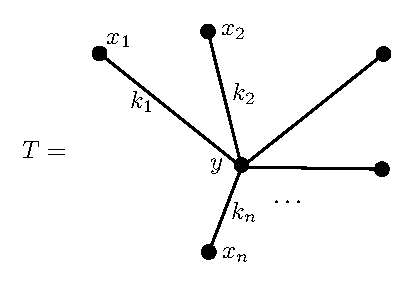
\includegraphics{grugraImages/GT1}
\end{center}
und $\GG$ enthält Gruppen $G_{x_i}$, $G_y=A$, $G_{k_i}=A$ und
Morphismen $\alpha_{k_i}:A\Ra G_i$.
Dann ist $G_T = \AST_A G_i$.
\end{enumerate}

\BEM $G_T$ ist wohldefiniert (hängt also nicht von der Wahl von
$x$ ab).

\textsc{Beweisskizze:} Fasse $\GG$ auf als \glqq induktives
System\grqq\
von Gruppen $G_x$, $G_k$ und Homomorphismenmengen $\Hom(G_x,G_y)=\emptyset$,
$\Hom(G_x,G_k)=\emptyset$, $\Hom(G_k,G_{\ini(k)})=\{\alpha_k\}$.

Dann gibt es einen induktiven Limes $G$ und Homomorphismen
$f_x:G_x\Ra G$, $f_k:G_k\Ra G$ mit
$f_{\ini(k)}\circ \alpha_k = f_k$ für alle $k\in K(T)$, so dass
die folgende UAE erfüllt ist: Zu jeder verträglichen Familie
von Homomorphismen $h_x:G_x\Ra H$, $h_k:G_k\Ra H$ gibt es genau einen
Homomorphismus $h:G\Ra H$ mit $h_x=h\circ f_x$ und $h_k=h\circ f_k$.
Dieser Limes ist $G_T$.
\qed

\FOLG Auch für einen unendlichen Baum $T$ kann man $G_T$ definieren.

\PROP\label{prop_BvG}
Es sei $\GG=(T,G_x,G_k,\alpha_k)$ ein Baum von Gruppen.
Dann gibt es einen (bis auf Isomorphie eindeutigen) Baum $\Xi$
und eine Aktion von $G_T$ auf $\Xi$, so dass gilt:
\begin{enumerate}
\item $T$ ist Fundamentalbereich für $\Xi/G_T$.
\item Für jedes $x\in E(T)$ ist $(G_T)_x = G_x$ und für jedes
$k\in K(T)$ ist $(G_T)_k = G_k$.
\end{enumerate}
Oder in anderen Worten: $\Xi/G_T \cong \GG$ als Graph von Gruppen.

\bew Zur Konstruktion von $\Xi$:
\begin{align*}
E(\Xi) &:= \BCUP{}{x\in E(T)} G_T/G_x, \\
K(\Xi) &:= \BCUP{}{k\in K(T)} G_T/G_k,
\end{align*}
und $\ini(gk):=g \ini(k)$, $\ter(gk):=g \ter(k)$ (man überzeuge sich,
dass dies wohldefiniert ist).

Es ist noch zu zeigen, dass $\Xi$ ein Baum ist. Ohne Einschränkung
können wir annehmen, dass $T$ endlich ist. Induktion über
$n:=|E(T)|$:\\
$n=1$: $\Xi=T$, $G_T=G_x$. Es ist nichts zu zeigen.\\
$n=2$: $T$ ist eine Segment der Form $(x,y;k)$. Dieser Fall wurde
in Satz \ref{satz_segment} betrachtet.\\
$n>2$: Es sei $x\in \ep(T)$ und $T':=T-x$. Dann ist
$G_T=G_{T'}*_{G_k} G_x$. Nun sei $\Xi' := G_{T'} T' \subset \Xi$.
Für $T'$ erfüllt $\Xi'$ die Voraussetzungen der Proposition.
Nun folgt mit der Induktionsannahme, dass $\Xi'$ ein Baum ist.
Für $g\in G_T$ ist
\[
g\Xi' \cap \Xi' =
\left\{
\begin{matrix}
\Xi', &  g\in G_{T'}, \\
\emptyset, & g\not\in G_{T'}.
\end{matrix}\right.
\]
Folglich sind Teilbäume $g\Xi'$ von $\Xi$ disjunkt, wenn $g$ ein
Vertretersystem der Nebenklassen in $G_T/G_{T'}$ durchläuft.
Es sei $\tilde{\Xi}$ der Graph, der aus $\Xi$ durch
Kontraktion alle $g \Xi'$ entsteht. $G_T$ operiert auf $\tilde{\Xi}$
mit Fundamentalbereich $T/T'=(T',x;k)$.
Dabei sind die Fixgruppen $G_{T'}$, $G_k$ und $G_x$.
Nach Satz \ref{satz_segment} (d.h. dem Fall $n=2$) folgt:
$\tilde{\Xi}$ ist ein Baum und damit nach
Proposition \ref{prop_wald} auch $\Xi$.
\qed

\PROP \label{prop_fundbereich}
Es sei $\rho:G\Ra\Aut(\GR)$ eine inversionsfreie Aktion,
so dass $\GR/G$ ein Baum ist (es gibt also einen Fundamentalbereich
$T\subset \GR$).
Weiter sei $\GG=(T,G_x,G_k,\alpha_k)$ der Baum von Gruppen zu
$\GR/G$, $G_T$ die Fundamentalgruppe von $\GG$ und $\Xi$ der
Baum zu $\GG$ aus Proposition \ref{prop_BvG}. Dann gilt:
\begin{enumerate}
\item Der durch die Inklusionen $G_x \hookrightarrow G$,
$G_k \hookrightarrow G$ induzierte Homomorphismus
$\phi:G_T \Ra G$ ist genau dann surjektiv, wenn $\GR$
zusammenhängend ist.
\item $\id:T\Ra T$ induziert einen Morphismus $f:\Xi\Ra\GR$,
der äquivariant\index{Morphismus!äquivariant} bzgl. der Aktionen von
$G_T$ bzw. $G$ ist, d.h. für $g\in G_T$ und $x\in E(T)$ gilt
$f(gx)=\phi(g)x$.
\item Die folgenden Aussagen sind äquivalent:
\begin{enumerate}
\item $\GR$ ist ein Baum.
\item $f$ ist ein Isomorphismus.
\item $\phi$ ist ein Isomorphismus.
\end{enumerate}
\end{enumerate}

\bew \begin{enumerate}
\item \glqq$\ra$\grqq: Ist $\phi$ surjektiv, so ist nach Teil 2 auch
$f$ surjektiv. Da $\Xi$ zusammenhängend ist, ist auch $\GR$
zusammenhängend.

\glqq$\la$\grqq: Dies ist ein Spezialfall ($T=Z$) der folgenden
Proposition \ref{prop_Gx_erzeugt}.
\item Klar.
\item
\glqq (b)$\ra$(a)\grqq: Klar.

\glqq (c)$\ra$(b)\grqq: Da $G_T\cong G$, enstpricht dies der 
Eindeutigkeit von $\Xi$ in Proposition \ref{prop_BvG}.

\glqq (a)$\ra$(b)\grqq: Für alle $x$ und $k$ sind
$\phi|_{G_x}$ und $\phi|_{G_k}$ Isomorphismen.
Daraus folgt, dass $f$ lokal injektiv ist (d.h. die Einschränkung
von $f$ auf einen \glqq Stern\grqq\ um $x$ ist injektiv für jedes
$x\in E(\Xi)$).
Wäre $f$ nicht injektiv, so gäbe es einen \glqq injektiven Weg\grqq\
$w$ in $\Xi$, so dass $f(w)$ nicht injektiv ist.
Da $\GR$ ein Baum ist, muss $f(w)$ einen Stachel haben.
\begin{center}
	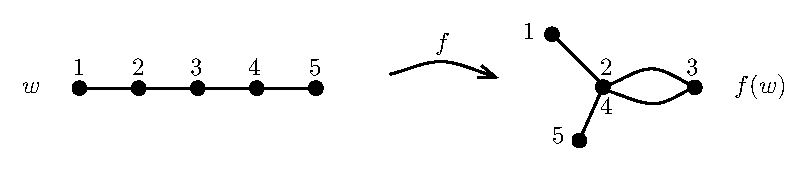
\includegraphics{grugraImages/winjektiv}
\end{center}
Dies ist aber ein Widerspruch zur lokalen Injektivität von $f$.
Somit muss $f$ injektiv sein.

$f$ ist auch surjektiv, da $\GR$ zusammenhängend ist und damit nach
Teil 1 $\phi$ surjektiv ist.

\glqq (b)$\ra$(c)\grqq: Ist $g\in\K{\phi}$, so ist $f(gx)=x$
für alle $x\in E(T)$. Da $f$ injektiv ist, muss $gx=x$ sein,
also $g\in G_x$ für alle $x\in E(T)$. Aus $\phi|_{G_x}=\id$
folgt $g=1$. Also ist $\phi$ injektiv und nach Teil 1 auch
surjektiv.
\qed
\end{enumerate}

\PROP \label{prop_Gx_erzeugt}
Es sei $\GR$ ein zusammenhängender Graph, $\rho:G\Ra\Aut(\GR)$
eine inversionsfreie Aktion, $T$ der Lift eines maximalen
Teilbaums von $\GR/G$, und $Z$ sei ein Teilgraph von $\GR$ mit
$T\subset Z$, $GZ=\GR$ derart, dass jede Kante in $Z$ mindestens
einen Eckpunkt in $T$ hat.
Für jede Kante $k\in K_0 := K(Z)-K(T)$ mit $\ini(k)\in E(T)$
sei $g_k\in G$ mit $g_k \ter(k)\in E(T)$.
Dann wird $G$ von den $G_x$, $x\in E(T)$, und den $g_k$, $k\in K_0$,
erzeugt.

\bew Es sei $H$ die von den $G_x$ und $g_k$ erzeugte Untergruppe.
Nun genügt es zu zeigen, dass $H E(T)=E(\GR)$ ist (denn für $g\in G$,
$x\in E(T)$ gibt es $h\in H$ mit $hx=gx$, also
$g^{-1}h\in G_x \leq H$, also $g\in H$).\\
Es gilt $E(Z)\subseteq H E(T)$, denn für $z\in E(Z)-E(T)$ gibt es
$k\in K_0$ mit $z=\ter(k)$, also $g_k z \in E(T)$.
Also ist nur noch zu zeigen, dass $HE(Z)=E(\GR)$ ist.
Dazu sei $x\in E(\GR)$. Ohne Einschränkung können wir $x=\ter(k)$
für eine Kante $k\in K(\GR)$ mit $\ini(k)\in HE(Z)$ annehmen,
da $\GR$ zusammenhängend ist. Außerdem können wir ohne Einschränkung
$\ini(k)\in E(T)$ annehmen (andernfalls ersetze $k$ durch ein
geeignetes $h^{-1}k$).
Nach Voraussetzung gibt es ein $g\in G$ mit $gk\in K(Z)$.
Zu zeigen ist nun, dass $g$ in $H$ liegt. Dazu unterscheiden wir
zwei Fälle:
\begin{itemize}
\item
$\ini(gk)\in E(T)$: Es ist $\ini(gk)=g\ini(k)$, $T$ ist Lift eines
maximalen Teilbaums und somit $g\ini(k)=\ini(k)$.
Also ist $g\in G_{\ini(k)}\leq H$.\\
\item
$\ter(gk)\in E(T)$: Dann ist $g_{\bar{k}} \ini(gk)\in E(T)$
und somit $g_{\bar{k}} g \in G_{\ini(k)}\leq H$.
Daraus folgt $g\in H$.
\qed
\end{itemize}


% ===============
\section{HNN-Erweiterungen}\label{sec_hnn}

Wir betrachten die \glqq Schleife von Gruppen\grqq\ zu
\begin{center}
	\includegraphics{grugraImages/L}
\end{center}
mit Gruppen $G_x$, $G_k=A$ und Homomorphismen
$\alpha_k:A\Ra G_x$ und $\alpha_{\bar{k}}:A\Ra G_x$.

Gesucht sind im Folgenden ein Baum $\Xi$ und eine Gruppe $G$,
die auf $\Xi$ operiert, so dass
$\GG(\Xi/G) = (L,G_x,A,\alpha_k,\alpha_{\bar{k}})$ gilt.

\BSP\
\begin{enumerate}
\item Es sei $G_x=\{1\}$. Dann ist $\Xi$ die unendliche Kette
und $G=\ZZ$ operiert auf $\Xi$ durch Translation.
\item Es sei $G_x=\ZZ/2\ZZ=\{1,\sigma\}$ und $A=G_x$,
$\alpha_k=\alpha_{\bar{k}}=\id$. Wieder ist $\Xi$ die
unendliche Kette. Die Gruppe $G$ wird erzeugt von der
Translation $\tau$ und einem Element $\sigma$ der Ordnung $2$,
dass trivial operiert.
Da $\tau\sigma\tau^{-1}$ alle Ecken fest lässt, gilt die Relation
$\tau\sigma\tau^{-1}=\sigma$, also
\[
G = \lag \tau,\sigma | \tau\sigma=\sigma\tau, \sigma^2=1 \rag.
\]
\item Es sei $G_x=\ZZ/2\ZZ=\{1,\sigma\}$ und $A=\{1\}$.
Der Baum $\Xi$ hat die Form
\begin{center}
	\includegraphics{grugraImages/XiF2}
\end{center}
Der Baum $\Xi$ ist der
Cayley-Graph der freien Gruppe $F_2$.
Wieder wird $G$ von Elementen $\tau$ und $\sigma$ erzeugt, wobei
$\tau$ durch Translation operiert und $\sigma$ die Ecke $x$
festlässt, aber $\tau x$ bewegen muss (wegen der Inversionsfreiheit
aber nicht auf $\tau^{-1} x$.
Es ist $\sigma^2=1$. Es gilt
\[
G = \lag \tau \rag * \lag \sigma \rag
= \ZZ * \ZZ/2\ZZ.
\]
Auf der vertikalen Achse operiert $\sigma\tau\sigma$ durch
Translation. Die von $\tau$ und $\sigma\tau\sigma$ erzeugte
Untergruppe ist $F_2$, denn sie operiert frei auf $\Xi$.
\end{enumerate}

\PROP\label{prop_hnn1}
Es seien $A$ und $G$ Gruppen und $\alpha_1,\alpha_2:A\Ra G$
injektive Homomorphismen.
Dann gibt es eine Gruppe $H$ mit $G\leq H$ und ein Element $t\in H$,
so dass für alle $a\in A$ gilt:
\[
\alpha_2(a) = t \alpha_1(a) t^{-1}.
\]
\bew Es sei $G'$ der induktive Limes des System
$(G_n, A_n, \alpha_{1,n}, \alpha_{2,n})_{n\in \ZZ}$,
wobei $G_n:=G$, $A_n:=A$, $\alpha_{1,n}:=\alpha_1:A_n\Ra G_{n-1}$
und $\alpha_{2,n}:=\alpha_2:A_n\Ra G_n$ sei.
Weiter seien $\iota_n:G_n \hookrightarrow G'$ die kanonischen Einbettungen.
\begin{center}
	\includegraphics{grugraImages/Glimes}
\end{center}
Weiter sei $u_n$ die Abbildung
$G_{n-1}\os{\Ra}{\id} G_n \os{\hookrightarrow}{\iota_n} G'$. Dann ist
$u_n(\alpha_{1,n}(a))=\iota_n(\alpha_{2,n}(a))$ für $a\in A_n$.
Wegen der UAE von $G'$ gibt es einen Automorphismus
$u:G'\Ra G'$ mit $u|_{G_{n-1}}=u_n$.
Sei $t$ das Element, dass auf $G'$ durch $u$ operiert, dann ist $\ZZ=\lag t \rag$.
Setze
\[
H := G' \ltimes_u \ZZ,
\]
d.h. als Menge ist $H=G'\times \ZZ$ und die Verknüpfung auf $H$
ist durch
\[
(g_1, n_1) \cdot (g_2, n_2) := (g_1 u^{n_1}(g_2), n_1+n_2)
\]
gegeben.
Für $g\in G'$ ist dann
\[
t g t^{-1} = (1,1)(g,0)(1,-1)
= (u(g),1)(1,-1) = (u(g),0).
\]
Insbesondere gilt für $a\in A$:
$t \alpha_1(a) t^{-1} = u(\alpha_1(a)) = \alpha_2(a)$.
\qed

\DB Die Gruppe $H$, die im Beweis zur Proposition \ref{prop_hnn1}
konstruiert wurde, ist universell bzgl. der Eigenschaften
in Proposition \ref{prop_hnn1}.
Sie heißt \emph{HNN-Erweiterung}\index{HNN-Erweiterung}
\[
H = \HNN(G,A,\alpha_1,\alpha_2)
\]
von $G$ bzgl. $A$, $\alpha_1$, $\alpha_2$
(benannt nach Graham Higman, Bernhard H. Neumann und Hanna Neumann).

\PROP \label{prop_hnn2}
Es sei $\GG=(L,G,A,\alpha_k,\alpha_{\bar{k}})$ eine Schleife von
Gruppen. Dann gibt es einen (bis auf Isomorphie eindeutigen)
Baum $\Xi$ und eine Aktion von $H=\HNN(G,A,\alpha_k,\alpha_{\bar{k}})$
auf $\Xi$, so dass $\GG(\Xi/H)\cong \GG$.
Die Gruppe $H$ heißt \emph{Fundamentalgruppe}\index{Fundamentalgruppe}
von $\GG$.

\bew Es sei $\Xi$ der Graph mit
\begin{align*}
E(\Xi) &= H/G, \\
K(\Xi) &= H/A \cup \bar{H/A},
\end{align*}
wobei $G$ als Untergruppe von $G'\leq H$ mit $G_0$ identifiziert wird,
entsprechend $A$ mit $A_1$.
Es ist $\ini(hA)=hG$ und $\ter(hA)=htG$.
Die Gruppe $H$ operiert durch Linksmultiplikation auf $\Xi$.
Es ist $\GG(\Xi/H)=L$ mit $x=1\cdot G$ und $k=1\cdot A$.
Dann ist $G_x=G$, $G_k=A$, $\alpha_k=\alpha_1$ und
$\alpha_{\bar{k}}=\alpha_2$.

Zu zeigen bleibt, dass $\Xi$ ein Baum ist: $G' \unlhd H$ operiert auf
$\Xi$ mit Quotientengraph $\Xi/G'$ mit
\begin{align*}
E(\Xi/G') &= (H/G)/G' \us{=}{G\leq G'} H/G' \cong \ZZ, \\
K(\Xi/G') &= H/G' \cup \bar{H/G'}.
\end{align*}
Also ist $\Xi/G'$ eine unendliche Kette mit Fixgruppen
$G_n\cong G$ bzw. $A_n\cong A$.
Auf $\Xi/G'$ operiert $H/G'$ durch Translation.
Nach dem Beweis von Proposition \ref{prop_hnn1} ist $G'$
Fundamentalgruppe von $\Xi/G'$.
Nun ist $\Xi$ nach Proposition \ref{prop_fundbereich} ein Baum.
\qed


% ================ 
\section{Fundamentalgruppe eines Graphen von Gruppen}\label{sec_FG_GvG}

\DB\label{def_FG2}
Es sei $\GG=(\GR,G_x,G_k,\alpha_k,\alpha_{\bar{k}})$ ein Graph
von Gruppen und $T$ ein maximaler Teilbaum von $\GR$.
Weiter sei $\pi_1(\GG,T)$ die Gruppe, die erzeugt wird
von den $G_x$, $x\in E(\GR)$, und Elementen $g_k$, $k\in K(\GR)\backslash K(T)$,
mit den Relationen
\begin{enumerate}
\item $g_{\bar{k}}=g_k^{-1}$ für alle $k\in K(\GR)\backslash K(T)$.
\item $\alpha_k(a)=\alpha_{\bar{k}}(a)$ für alle $k\in K(T)$ und
$a\in G_k$.
\item $g_k \alpha_{\bar{k}}(a) g_k^{-1} = \alpha_k(a)$
für alle $k\in K(\GR)\backslash K(T)$ und $a\in G_k$.
\end{enumerate}
$\pi_1(\GG,T)$ heißt \emph{Fundamentalgruppe}\index{Fundamentalgruppe}\index{$\pi_1(\GG,T)$, $\pi_1(\GG)$ (Fundamentalgruppe)}
von $\GG$ (bzgl. $T$).

\BSP Fundamentalgruppen.
\begin{enumerate}
\item Ist $\GR=T$, so ist 
\[
\pi_1(\GG,T)=G_T
\]
(vgl. Abschnitt \ref{sec_BvG}).
\item Ist $\GR=L$ (aus Abschnitt \ref{sec_hnn}), so ist $T=\{x\}$ und
\[
\pi_1(\GG,\{x\})=\HNN(G,A,\alpha_k,\alpha_{\bar{k}}).
\]
\end{enumerate}

\SATZ \label{satz_cover}\
\begin{enumerate}
\item Es sei $\GG=(\GR,G_x,G_k,\alpha_k,\alpha_{\bar{k}})$ ein
Graph von Gruppen.
Dann gibt es einen (bis auf Isomorphie eindeutigen) Baum $\Xi$
und eine Aktion $\rho$ von $G=\pi_1(\GG,T)$ auf $\Xi$, so dass
$\GG(\Xi/G)=\GG$ (dabei sei $T$ ein beliebiger maximaler Teilbaum
von $\GR$). Das Paar $(\Xi,\rho)$ heißt
\emph{universelle Überlagerung}\index{universelle Überlagerung}
von $\GG$.
\item Es sei $\Xi$ ein Baum und $G$ eine Gruppe, die inversionsfrei
auf $\Xi$ operiert. Dann ist $G\cong \pi_1(\GG(\Xi/G),T)$
(bzgl. eines beliebigen maximalen Teilbaums $T$ von $\Xi/G$).
\end{enumerate}

Bevor wir diesen Satz beweisen, soll zunächst die (Un-)Abhängigkeit
der Fundamentalgruppe vom Baum $T$ geklärt werden.
Dies wird sich auch im Beweis des Satzes als hilfreich erweisen.
Dabei verwenden wir durchgehend die Bezeichnungen aus Definition
\ref{def_FG2}.

\DEF Für $\GG$ sei $\F(\GG)$\index{$\F(\GG)$} die
Gruppe, die erzeugt wird von $G_x$, $x\in E(\GR)$, und Elementen
$g_k$, $k\in K(\GR)$, mit den Relationen
\begin{enumerate}
\item $g_{\bar{k}}=g_k^{-1}$
\item $g_k \alpha_{\bar{k}}(a) g_k^{-1} = \alpha_k(a)$
\end{enumerate}
für alle $k\in K(\GR)$ und $a\in G_k$.

\BEM\label{bem_p}
Ist $T$ ein maximaler Teilbaum von $\GR$, so induziert
$\id_x:G_x\Ra G_x$,
$g_k\mapsto
\left\{\begin{matrix}
1, & k\in K(T) \\
g_k, & k\not\in K(T)
\end{matrix}\right.$, einen surjektiven Homomorphismus
$p:\F(\GG)\Ra \pi_1(\GG,T)$.
Der Kern von $p$ ist der Normalteiler, der von den $g_k$, $k\in K(T)$,
erzeugt wird.

\DEF\
\begin{enumerate}
\item Es sei $w=(k_1,\ldots,k_n)$ ein Weg in $\GR$, $x_0:=\ini(k_1)$,
$x_i:=\ter(k_i)$($=\ini(k_{i+1})$) für $i=1,\ldots,n$.
Ein Element $g\in\F(\GG)$ heißt \emph{vom Typ}\index{Typ} $w$,
wenn es $h_i\in G_{x_i}$ (für $i=0,\ldots,n$) gibt mit
\[
g = h_0 g_{k_1} h_1 g_{k_2} \cdots g_{k_n} h_n.
\]
\item Setze
\[
\pi_1(\GG,x_0) :=
\{ g\in\F(\GG) : \text{ $g$ ist vom Typ $w$ für einen Weg $w$ mit
$\ini(w)=x_0=\ter(w)$} \}.
\]
\end{enumerate}

\BSP Sind alle $G_x=\{1\}$, so ist $\pi_1(\GR,x_0)$ die
Fundamentalgruppe wie in Abschnitt \ref{sec_FG} (Stacheln ergeben
$g_k g_{\bar{k}}=1$).

\BEM Die Abbildung
\[
\beta:\pi_1(\GG,x_0) \Ra \pi_1(\GR, x_0),\quad
h_0 g_{k_1} h_1 g_{k_2} \cdots g_{k_n} h_n \mapsto
g_{k_1} g_{k_2} \cdots g_{k_n}
\]
ist ein surjektiver Gruppenhomomorphismus.
$\K{\beta}$ ist der von den $G_x$ erzeugte Normalteiler.

\BEM\label{bem_pi1}
Es sei $\GG$ ein Graph von Gruppen, $x_0\in E(\GR)$ und
$T\subset \GR$ ein maximaler Teilbaum. Dann ist
\[
p|_{\pi_1(\GG,x_0)}:\pi_1(\GG,x_0)\Ra \pi_1(\GG,T)
\]
ein Isomorphismus.

\bew Für jedes $x\in E(T)=E(\GR)$ sei $w_x=(k_1,\ldots,k_n)$
der eindeutig bestimmte stachelfreie Weg in $T$ von $x_0$ nach $x$
und $\gamma_x:=g_{k_1}\cdots g_{k_n}\in\F(\GG)$.
Definiere die Abbildung $f:\pi_1(\GG,T)\Ra\F(\GG)$ durch
\begin{align*}
f(h) &:= \gamma_x h \gamma_x^{-1}\quad \text{ für } h\in G_x, \\
f(g_k) &:= \gamma_{\ini(k)} g_k \gamma_{\ter(k)}^{-1}
\quad \text{ für } g_k \text{ mit } k\in K(\GR)\backslash K(T).
\end{align*}
Der durch $f$ gegebene Homomorphismus respektiert die
Relationen in $\F(\GG)$:
\begin{enumerate}
\item $f(g_{\bar{k}})
=\gamma_{\ini(\bar{k})} g_{\bar{k}} \gamma_{\ter(\bar{k})}^{-1}
=\gamma_{\ter(k)} g_k^{-1}\gamma_{\ini(k)}^{-1}
=(\gamma_{\ini(k)} g_k \gamma_{\ter(k)}^{-1})^{-1}
=f(g_k)^{-1}$.
\item Für $k\in K(T)$ ist $\gamma_{\ter(k)}=\gamma_{\ini(k)} g_k$.
Für $a\in G_k$ ist dann
\begin{align*}
f(\alpha_k(a)) &= \gamma_{\ini(k)} \alpha_k(a) \gamma_{\ini(k)}^{-1}, \\
f(\alpha_{\bar{k}}(a))
&= \gamma_{\ini(\bar{k})} \alpha_{\bar{k}}(a) \gamma_{\ini(\bar{k})}^{-1} \\
&= \gamma_{\ini(k)} \ub{g_k \alpha_{\bar{k}}(a) g_k^{-1}}{=\alpha_k(a)} \gamma_{\ini(k)}^{-1} \\
&= f(\alpha_k(a)).
\end{align*}
\item Für $k\in K(\GR)\backslash K(T)$ ist
\begin{align*}
f(\alpha_k(a)) &= \gamma_{\ini(k)} \alpha_k(a) \gamma_{\ini(k)}^{-1}, \\
f(g_k \alpha_{\bar{k}}(a) g_k^{-1})
&= (\gamma_{\ini(k)}g_k \gamma_{\ter(k)}^{-1})
(\gamma_{\ini(\bar{k})}\alpha_{\bar{k}}(a)\gamma_{\ini(\bar{k})}^{-1})
(\gamma_{\ter(k)}g_k^{-1}\gamma_{\ini(k)}^{-1})\\
&= \gamma_{\ini(k)} g_k \alpha_{\bar{k}}(a) g_k^{-1}\gamma_{\ini(k)}^{-1} \\
&= \gamma_{\ini(k)}\alpha_{k}(a)\gamma_{\ini(k)}^{-1}.
\end{align*}
\end{enumerate}
Also definiert $f$ einen Homomorphismus, dessen Bild in
$\pi_1(\GG,x_0)$ liegt. Dieser Homomorphismus ist surjektiv:\\
Es ist $p(\gamma_x)=1$ für alle $x\in E(\GR)$ und $p\circ f=\id$.
Sei $g=h_0 g_{k_1} h_1 g_{k_2} \cdots g_{k_n} h_n\in\pi_1(\GG,x_0)$.
Dann ist
$f(p(g))=g$.
\qed

\FOLG Für maximale Teilbäume $T$ und $T'$ von $\GR$ ist
\[
\pi_1(\GG,T) \cong \pi_1(\GG,T').
\]
Entsprechend ist $\pi_1(\GG,x_0)\cong\pi_1(\GG,x_1)$.

Nun wenden wir uns dem Beweis des Satzes \ref{satz_cover} zu.
Es sei $G:= \pi_1(\GG,T)$.
Zuerst betrachten wir die Konstruktion des Graphen $\Xi$:
\begin{align*}
E(\Xi) &:= \BCUP{.}{x\in E(\GR)} G/G_x, \\
K(\Xi) &:= \BCUP{.}{k\in K(\GR)} G/G_k.
\end{align*}
Für $gk\in K(\Xi)$ sei $\bar{gk}:=g\bar{k}$.
Für $k\in K(T)$ setze $\ini(gk):=g\ini(k)$ und
$\ter(gk):=g\ter(k)$.
Für die Kanten $k\in K(\GR)\backslash K(T)$ ist die Sache 
komplizierter, wie die folgenden Skizzen veranschaulichen:
\begin{center}
	\includegraphics{grugraImages/T01}
\end{center}
Der Baum $T$ wird zu einem Baum $T_0$ in $\Xi$ geliftet, der
über den Lift der Kante $k$ mit einer Kopie von $T_0$ verbunden ist.
Ebensogut hätte man aber über einen Lift der Kante $\bar{k}$
mit einer Kopie von $T$ verbinden können:
\begin{center}
	\includegraphics{grugraImages/T02}
\end{center}
Man muss sich also bei jeder geometrischen Kante $\{k,\bar{k}\}$
für $k$ oder $\bar{k}$ entscheiden, d.h. wir müssen eine Orientierung
$K^+ := (K(\GR)\backslash K(T))^+$ wählen.
Nun setzen wir für $k\in K^+$:
\begin{align*}
\ini(gk) &:= g \ini(k), \\
\ter(gk) &:= g g_k \ter(k)
\end{align*}
und schließlich
\begin{align*}
\ini(g\bar{k}) &:= g g_k \ini(\bar{k}), \\
\ter(g \bar{k}) &:= g \ter(\bar{k}).
\end{align*}
Nach Konstruktion gilt nun
\[
\ini(\bar{gk}) = g g_k \ini(\bar{k}) = g g_k \ter(k)
= \ter(gk).
\]
Diese Definitionen sind unabhängig von der Wahl eines Repräsentanten
einer Nebenklasse: Ist $h\in G_k$, so ist $g h k = g k$.
Also muss gelten:
\[
g h \ini(k) = g \ini(k),
\]
da $h\in G_k \leq G_{\ini(k)}$. Entsprechend sieht man dies
für $\ter(k)\in E(T)$.
Für $\ter(k)\not\in E(T)$ gilt:
\[
g h g_k \ter(k) = g g_k \ter(k),
\]
da $ g_k^{-1} h g_k = \alpha_{\bar{k}}(h) \in G_{\ter(k)}$,
also $h g_k = g_k h'$ für ein geeignetes $h'\in G_{\ter(k)}$.

Somit haben wir den Graphen $\Xi$ aus Teil 1 von Satz \ref{satz_cover}
und eine Aktion von $G$ auf $\Xi$, so dass $\GG(\Xi/G)\cong \GG$.
Im Folgenden wird gezeigt werden, dass $\Xi$ wie behauptet ein Baum
ist.

\BEM $\Xi$ ist zusammenhängend.

\bew Es sei $T_0 \subset \Xi$ ein Lift von $T$ (vgl. die Skizzen 
oben), d.h.
\begin{align*}
E(T_0) &= \{ 1x : x\in E(\GR)=E(T) \}, \\
K(T_0) &= \{ 1k : k\in K(T) \}.
\end{align*}
Weiter sei $T_1$ der kleinste Teilgraph von $\Xi$, der $T_0$ enthält
und alle Kanten $1k$ sowie $1\bar{k}$ für $k\in K^+$.
\begin{center}
	\includegraphics{grugraImages/T0T1}
\end{center}
$T_1$ ist zusammenhängend: $\ini(1k)=\ini(k)\in E(T_0)$.
Weiter gilt  $GT_1 = \Xi$. Die Menge
\[
S = \{g_k : k\in K^+ \} \cup \BCUP{}{x\in E(\GR)} G_x
\]
erzeugt $G$. Sei nun $g\in S$. Ist $g \in G_x$, so ist
$1x \in T_1 \cap g T_1$, da $G_{1x}=G_x$.
Ist $g=g_k$, so ist $\ter(1k)=g_k \ter(k) \in E(T_1 \cap g_k T_1)$,
also $g T_1 \cap T_1 \neq \emptyset$.

Mit Induktion über die Wortlänge in $G$ (bzgl. $S$) folgt,
dass $T_1$ zusammenhängend ist (und damit auch $\Xi$).
\qed

\DEF\
\begin{enumerate}
\item Eine Folge $(h_0,g_{k_1},\ldots,g_{k_n},h_n)$ heißt
\emph{Wort vom Typ} $w$, wenn $g=h_0 g_{k_1}\cdots g_{k_n} h_n$
vom Typ $w$ ist.\index{Wort!vom Typ $w$}\index{Typ}
\item Ein Wort heißt \emph{reduziert}\index{Wort!reduziert}\index{reduziertes Wort},
wenn für alle Stachel, also alle $i$ mit $k_{i+1}=\bar{k}_i$, gilt:
$h_i\not\in \alpha_{\bar{k}_i}(G_{\bar{k}_i})$, falls $n\geq 1$.
(Falls $n=0$, so heiße $h_0$ reduziert, wenn $h_0\neq 1$.)
\end{enumerate}

\PROP\label{prop_nicht_eins}
Ist $c=(h_0,g_{k_1},\ldots,g_{k_n},h_n)$ ein reduziertes Wort
von Typ $w$ für $w=(k_1,\ldots,k_n)$ in $\GR$, so ist
\[
g(c) = h_0 g_{k_1}\cdots g_{k_n} h_n \in \F(\GG)\backslash\{ 1 \}.
\]

Der umfangreiche Beweis dieser Proposition folgt am Ende
des Abschnitts.

\FOLG Ist $w$ ein geschlossener Weg in $\GR$, so ist $p(g)\neq 1$
in $\pi_1(\GG,T)$ für jedes zu einem reduzierten Wort vom Typ $w$
gehörende $g\in \F(\GG)$ (mit $p$ aus Bemerkung \ref{bem_p}).

\bew Für $x_0 := \ini(w)$ gilt $g\in \pi_1(\GG,x_0)$.
Da $p|_{\pi_1(\GG,x_0)}$ injektiv ist (nach Bemerkung \ref{bem_pi1}),
folgt $p(g)\neq 1$, da $g\neq 1$.
\qed

Wir schließen nun den Beweis von Teil 1 von Satz \ref{satz_cover} ab.
\BEM $\Xi$ enthält keine stachelfreien geschlossenen
Wege und ist somit ein Baum.

\bew Wir nehmen an, es gäbe einen stachelfreien geschlossenen Weg
$w'=(k_1',\ldots,k_n')$ in $\Xi$.

Es sei $k_i' = s_i k_i$ mit $k_i \in K(\GR)$ und $s_i\in G$.
Setze
\[
\eps_i := \left\{
\begin{matrix}
0, & k_i \in K^+ \\
1, & \text{sonst}
\end{matrix}\right.
\]
Schreibe $g_i := g_{k_i}$. Dann ist
\begin{align*}
& \ter(k_n') = \ter(s_n k_n) = s_n g_n^{1-\eps_n} \ter(k_n) \\
=\ & \ini(k_1')=s_1 g_1^{-\eps_1}\ini(k_1)=s_1 g_1^{-\eps_1}\ter(k_n),
\end{align*}
also $s_n g_n^{-\eps_n} g_n r_n = s_1 g_1^{-\eps_1}$ für ein
$r_n \in G_{\ini(k_1)}=G_{\ter(k_n)}$.
Analog: $s_i g_i^{-\eps_i} g_i r_i = s_{i+1} g_{i+1}^{-\eps_{i+1}}$
für ein $r_i\in G_{\ter(k_i)}=G_{\ini(k_{i+1})}$.
Mit $q_i := s_i g_i^{-\eps_i}$ gilt:
\[
g_i r_i = q_i^{-1} q_{i+1}
\]
für $i=1,\ldots, n-1$.
Es folgt
\[
g_1 r_1 g_2 r_2 \cdots g_n r_n = 1.
\]
Aber $(1,g_1,r_1,\ldots,g_n,r_n)$ ist ein reduziertes Wort vom Typ
$w$ ($=$ Bild von $w'$ in $\GR$).
Dies ist ein Widerspruch zur Proposition \ref{prop_nicht_eins}.
Es kann also keine stachelfreien geschlossenen Wege in $\Xi$ geben.
\qed

\textsc{Beweis von Proposition \ref{prop_nicht_eins}:}
Wir betrachten drei Fälle:
\begin{enumerate}
\item
$\GR$ ist das Segment $(x_1,x_2;k)$ mit Gruppen
$G_1$, $G_2$ und $A=G_k$. Dann hat jeder Weg die Form
\[
w = (l,\bar{l},\ldots,l(,\bar{l}))
\]
mit $l\in\{ k, \bar{k} \}$.
Ein reduziertes Wort von Typ $w$ ist
\[
c = (h_0,g,h_1,g^{-1},\ldots,h_n)
\]
mit $h_i\in G_1$ für gerades $i$, $h_i\in G_2$ für ungerades $i$
und $h_i\not\in A$ für $i\geq 1$.

Das Bild $g(c)$ von $c$ in $\pi_1(\GG)$ ist
$h_0 h_1\cdots h_n \in G_1 *_A G_2=\pi_1(\GG)$.
Nach Bemerkung \ref{bem_NF} ist $g(c)\neq 1$.

\item
$\GR$ ist die Schleife $L$. Hier ist
\[
w = (k^{\eps_1},k^{\eps_2},\ldots,k^{\eps_n})
\]
mit $\eps_i\in\{-1,1\}$ und $k^{-1}:=\bar{k}$.

Ein Wort $c=(h_0,g^{\eps_1},\ldots,g^{\eps_n},h_n)$ ist reduziert,
wenn $h_i\not\in \alpha_{\bar{k}_i}(A)$, falls $\eps_{i+1}=-\eps_i$.
Nach dem Beweis von Proposition \ref{prop_hnn1} ist
$h_0 g^{\eps_1}\cdots g^{\eps_n}h_n\neq 1$ in $\pi_1(\GG)$.

\item
Der allgemeine Fall für $\GR$. Hier ist die Idee, Induktion
zu verwenden und den Fall für $\GR$ auf ein geeignetes $\GR/Y$
zurückzuführen, indem man ein Segment oder eine Schleife in $\GR$
kontrahiert. Um dabei keine Information zu verlieren, wird im
Graph von Gruppen ein Segment $(G_1,G_2;A)$ ersetzt durch
die Eckengruppe $G_1*_A G_2$, und eine Schleife wird durch eine
Eckengruppe $\HNN(G,A,\alpha_k,\alpha_{\bar{k}})$ ersetzt.

Es sei also $Y$ ein Teilgraph von $\GR$ mit genau einer geometrischen
Kante $\{k,\bar{k}\}$ (d.h. $Y$ ist Segment oder Schleife).
Weiter sei $\GG(Y)$ der Teilgraph von Gruppen
$(Y,G_1,G_2,A,\alpha_{k},\alpha_{\bar{k}})$ bzw.
$(Y,G,A,\alpha_{k},\alpha_{\bar{k}})$, und $G_Y=\pi_1(\GG(Y))$.
Es sei $\mathscr{H}$ der Graph von Gruppen
$(\GR/Y,G_x,G_k,\alpha_k,\alpha_{\bar{k}})$ mit
\[
G_x = \left\{
\begin{matrix}
G_x, & x\not\in E(Y) \\
G_Y, & x\in E(Y)
\end{matrix}\right.
\]
und $G_k$, $\alpha_k$, $\alpha_{\bar{k}}$ wie bisher.

Man überzeuge sich, dass
\[
\pi_1(\mathscr{H}) \cong \pi_1(\GG)
\]
gilt.

Es sei nun $w=(k_1,\ldots,k_n)$ ein Weg in $\GR$ und
$w'=(k_1',\ldots,k_m')$ das Bild von $w$ in $\GR/Y$.
Ist $c=(h_0,g_1,\ldots,g_n,h_n)$ ein Wort vom Typ $w$ in $\GG$,
so wähle
$c'=(h_0',g_1',\ldots,g_m',h_m')$ als zugehöriges Wort vom
Typ $w'$ in $\mathscr{H}$, wobei $g_i'=g_j$ für $k_i'=k_j$ und
$h_i'$ durch Iterieren der Vorschrift
\[
h_i' = \left\{
\begin{matrix}
h_j, &
\text{falls $k_i'=k_j$ und $k_{i+1}\not\in\{k,\bar{k}\}\ni k_i$}\\
h_i g_{i+1} h_{i+1}, &
\text{falls $k_{i+1}=k$ und $k_i\not\in\{k,\bar{k}\}$}
\end{matrix}\right.
\]
gegeben ist.

Wir zeigen nun, dass $c'$ reduziert ist, wenn $c$ reduziert ist
(dann folgt die Aussage mit Induktion über $|K(\GR)|$ bzw. $|w|$).

Verwende Induktion über $|w'|$:

$|w'|=0$: Ist $|w|>0$, so ist $w$ ein Weg in $Y$, also
$g(c')=g(c)\neq 1$ nach Fall 1 oder Fall 2.

Der Fall $|w'|>0$ sei dem Leser als Übung überlassen.
\qed
\end{enumerate}

% =============
\section{Der Satz von Kurosh}\label{sec_kurosh}

\SATZ \emph{(Satz von Kurosh)}\index{Kuroshs Satz}\index{Satz!Kurosh}\\
Es sei $G=\AST_{i\in I} G_i$ ein freies Produkt von Gruppen und
$H\leq G$ eine Untergruppe. Dann ist $H$ ein freies Produkt der
Form
\[
H = F * \us{\AST}{i\in I, x\in X_i} H_{i,x},
\]
wobei $X_i$ ein Vertretersystem der Doppelnebenklassen $H g G_i$ ist,
$H_{i,x} = H \cap x G_i x^{-1}$ und $F$ eine freie Gruppe.

\bew Es sei $\GR$ ein Baum mit Ecken $x_i$, $i\in I$, und
$\GG=(\GR,G_i,\{1\},\id,\id)$ ein Graph von Gruppen auf $\GR$.
Dann ist $\pi_1(\GG)=G$.
Nach Proposition \ref{prop_BvG} gibt es einen Baum $\Xi$ und
eine Aktion von $G$ auf $\Xi$, so dass $\GG(\Xi/G)\cong \GG$.
Die Gruppe $H$ operiert auch auf $\Xi$. Nach Teil 2 von
Satz \ref{satz_cover} gilt $H\cong \pi_1(\GG(\Xi/H))$.
Alle Kantengruppen sind $\{1\}$.
Es ist $F=\pi_1(\Xi/H)$ die freie Gruppe über $K(\Xi/H)\backslash K(T)$,
wobei $T$ ein maximaler Teilbaum von $\Xi/H$ ist.
Es ist
\[
E(\Xi)=\BCUP{.}{i\in I} G/G_i.
\]
Für $x=g G_i$ gilt:
\[
H_x = H \cap G_x = H \cap g G_i g^{-1}.
\]
Die Ecken von $\Xi/H$ sind die Bahnen von $E(\Xi)$ unter $H$:
\[
E(\Xi/H) = \{ H g G_i : g \in G/G_i, i\in I \}.
\]
Also ist $X_i=E(\Xi/H)$.
\qed

Die Aussage bleibt richtig für $G=\AST_A G_i$ und $H\cap A =\{1\}$.

\cleardoublepage
\part{Der Bruhat-Tits-Baum für $\GL_2(\QQ_p)$}

%===========
\section{$p$-adische Zahlen}\label{sec_padisch}

Es sei $p$ eine Primzahl. Eine Zahl $n\in\NN$ lässt sich eindeutig
schreiben als
\[
n = \SUM{k}{i=0} a_i p^i
\]
mit $a_i\in\{0,\ldots,p-1\}$ und $k\geq 0$.

\BEM\label{def_ubertrag}
Wir rechnen mit Übertrag: Für $n=\sum a_i p^i$ und
$m=\sum b_i p^i$ ist
\begin{gather*}
m+n = \sum c_i p^i, \\
mn = \sum d_i p^i
\end{gather*}
mit
$c_i = \tilde{c}_i - \rho_i p$,
$d_i = \tilde{d}_i - \sigma_i p$,
wobei 
\[
\tilde{c}_i=a_i+b_i+\rho_{i-1},\quad
\tilde{d}_i=(\sum_{l=0}^i a_l b_{i-l})+\sigma_{i-1}
\]
und
$\rho_i = \left\{\begin{matrix}
1, & \tilde{c}_i \geq p \\
0, & \tilde{c}_i < p
\end{matrix}\right.,$
$\sigma_i=\max\{s\in\NN:sp\leq \tilde{d}_i\}$
ist.

\DB Die Menge
\[
\ZZ_p = \left\{
\SUM{\infty}{i=0} a_i p^i : a_i \in \{0,\ldots,p-1\}
\right\}
\]
wird mit $+$ und $\cdot$ wie in Definition \ref{def_ubertrag}
zu einem kommutativen Ring mit $1$. Er heißt
\emph{Ring der ganzen $p$-adischen Zahlen}.\index{p-adische Zahlen!Ring}\index{$\ZZ_p$ ($p$-adische Zahlen)}

\bew Wir zeigen, dass $(\ZZ_p,+)$ eine Gruppe ist:
\begin{align*}
-(\sum a_i p^i) &= (p-a_0) + (p-a_1-1) p + (p-a_2-1) p^2 + \ldots \\
&= (p-a_0) + \SUM{\infty}{i=1} (p-a_i-1) p^i.
\end{align*}
Es gibt also zu jedem Element ein additiv Inverses.

Die übrigen Ringeigenschaften sind klar.
\qed

\PROP\ \begin{enumerate}
\item Die Inklusion $\NN\subset \ZZ_p$ induziert eine Einbettung
$\iota:\ZZ\hookrightarrow \ZZ_p$.
\item $\ZZ_p$ ist nullteilfrei.
\end{enumerate}
\bew \begin{enumerate}
\item Für $n\in\ZZ$, $n<0$, setze $\iota(n):=-\iota(-n)$.
\item Es seien $a=\sum a_i p^i, b=\sum b_i p^i \in \ZZ_p\backslash\{0\}$ und
\[
i_a := \min\{i:a_i \neq 0\},\quad
i_b := \min\{i:b_i \neq 0\}.
\]
Für $ab=\sum d_i p^i$ ist dann $\tilde{d}_{i_a+i_b}=a_{i_a}b_{i_b}$
nicht durch $p$ teilbar, da $p$ prim ist.
Folglich ist auch $d_{i_a+i_b}=\tilde{d}_{i_a+i_b}-\sigma_i p$
nicht durch $p$ teilbar und insbesondere $\neq 0$.
Also ist $ab\neq 0$.
\qed
\end{enumerate}

\BEM Es sei
\[
\mm_p = \left\{
a=\SUM{\infty}{i=0} a_i p^i \in \ZZ_p : a_0=0
\right\}.
\]
Dann gilt:
\begin{enumerate}
\item $\mm_p$ ist ein maximales Ideal.
\item $\ZZ_p/\mm_p \cong \ZZ/p\ZZ \cong \FF_p$.
\item $a\in \ZZ_p^\times$ genau dann, wenn $a\not\in\mm_p$.
\end{enumerate}
Insbesondere ist $\mm_p$ das einzige maximale Ideal in $\ZZ_p$,
d.h. $\ZZ_p$ ist ein lokaler Ring (vgl. Kapitel II.4 in 
Lang \cite{lang}).

\bew \begin{enumerate}
\item Offensichtlich ist $\mm_p$ ein Ideal. Die Maximalität
folgt aus Teil 2 oder 3.
\item Die Abbildung $a=\sum a_i p^i \mapsto \bar{a}_0\in \ZZ/p\ZZ$
ist ein surjektiver Ringhomomorphismus mit Kern $\mm_p$.
Der Homomorphiesatz liefert die Behauptung.
\item Es sei $a=\sum a_i p^i \in \ZZ_p\backslash \mm_p$, also
$a_0\neq 0$. Gesucht ist $b=\sum b_i p^i$ mit $ab=1$.
Definiere die $b_i$ induktiv: Da $p$ prim ist, kann man $b_0$ so 
wählen, dass $a_0 b_0 \equiv 1 \mod p$ gilt.
Hat man für $i\geq 1$ schon $b_0,\ldots,b_{i-1}$ gefunden, wähle
$b_i$ so, dass
\[
a_0 b_i + \SUM{i}{l=1} a_l b_{i-l} \equiv 0 \mod p
\]
gilt.
\qed
\end{enumerate}

\DB\
\begin{enumerate}
\item Der Quotientenkörper
\[
\QQ_p = \mathrm{Quot}(\ZZ_p)
\]
heißt \emph{Körper der $p$-adischen Zahlen}.\index{p-adische Zahlen!Körper}\index{$\QQ_p$ ($p$-adische Zahlen)}
\item Die Inklusion $\ZZ\hookrightarrow \ZZ_p$ induziert eine
Inklusion $\QQ\hookrightarrow \QQ_p$ (d.h. $\Char(\QQ_p)=0$).
\item Jedes $a\in \QQ_p^\times=\QQ_p\backslash\{0\}$ hat eine
eindeutige Darstellung
\[
a=\SUM{\infty}{i=i_a} a_i p^i
\]
mit $a_i\in\{0,\ldots,p-1\}$ und $i_a\in\ZZ$ minimal, so dass
$a_{i_a}\neq 0$.
\end{enumerate}
\textsc{Beweis von 3.:} Ist $a=\sum a_i p^i\in\ZZ_p\backslash\{0\}$,
so sei $i_a=\min\{i:a_i\neq 0\}$.
Dann ist $a=\SUM{\infty}{i=i_a} a_i p^i$ die gewünschte Darstellung.

Es ist $a=p^{i_a} u$ mit $u=\SUM{\infty}{i=0}a_{i+i_a} p^i\in\ZZ_p^\times$.
Nun sei $\frac{a}{b}\in\QQ_p$ mit $a,b\in\ZZ_p$, $b\neq 0$.
Schreibe $a=p^{i_a} u$ und $b=p^{i_b}v$ mit $i_a,i_b\in\NN$ und
$u,v\in\ZZ_p^\times$.
Es folgt
$\frac{a}{b}=p^{i_a-i_b} \ub{uv^{-1}}{\in\ZZ_p^\times}$,
wie gewünscht.
\qed

\DB\
\begin{enumerate}
\item Für $a=\SUM{\infty}{i=i_a}a_i p^i \in \QQ_p^\times$ sei
\begin{gather*}
\vv(a) := i_a,\\
|a| := p^{-i_a}.
\end{gather*}
\item Ist $a\in \ZZ$, so ist $\vv(a)=\max\{n:p^n|a\}$.
\item $a\in\ZZ_p\backslash\{0\}\ \lra\ \vv(a)\geq 0\ \lra\ |a|\leq 1$.
\item Setze $\vv(0):=\infty$, $|0|:=0$.
\item Für alle $a,b\in\QQ_p^\times$ gilt:
\begin{enumerate}
\item $\vv(ab)=\vv(a)+\vv(b)$ bzw. $|ab|=|a|\cdot |b|$.
\item $\vv(a+b)\geq\min\{\vv(a),\vv(b)\}$ bzw.
$|a+b|\leq\max\{|a|,|b|\}$.
\item Ist $\vv(a)\neq\vv(b)$, so ist $\vv(a+b)=\min\{\vv(a),\vv(b)\}$
bzw. $|a+b|=\max\{|a|,|b|\}$.
\item $\vv(a)=\vv(-a)$.
\end{enumerate}
\item $\vv:\QQ_p^\times \Ra \ZZ$ heißt \emph{$p$-adische Bewertung},
$|\cdot|:\QQ_p^\times \Ra \RR$ heißt \emph{$p$-adischer Betrag}.
\index{p-adische Bewertung}\index{p-adischer Betrag}\index{$\vv(a)$ ($p$-adische Bewertung)}
\end{enumerate}

\PROP\ \label{prop_schenkel}
\begin{enumerate}
\item $d(x,y):=|x-y|$ ist eine Metrik auf $\QQ_p$.
\item Jedes Dreieck in $\QQ_p$ ist gleichschenklig, und die dritte
Seite ist höchstens so lang wie einer der gleichen Schenkel.
\end{enumerate}
\bew
\begin{enumerate}
\item Es gilt
\begin{gather*}
d(x,y)=0\ \lra\ x-y=0\ \lra\ x=y,\\
d(y,x)=|y-x|=|-(x-y)|=|-1|\cdot|x-y|=d(x,y)\\
\text{und}\\
d(x,z)=|x-z|=|(x-y)+(y-z)|\leq\max\{|x-y|,|y-z|\}\leq d(x,y)+d(x,z).
\end{gather*}
\item Folgt aus $|x-z|\leq \max\{|x-y|,|y-z|\}$.
\qed
\end{enumerate}

\PROP\ \begin{enumerate}
\item $\QQ_p$ ist vollständig.
\item $\QQ$ liegt dicht in $\QQ_p$.
\end{enumerate}
\bew \begin{enumerate}
\item Es sei $(a^{(n)})$ eine Cauchy-Folge in $\QQ_p$,
\[
a^{(n)} = \SUM{\infty}{i=i_a(n)} a_i^{(n)} p^i,
\]
mit $a_i^{(n)}\in\{0,\ldots,p-1\}$ und
$i_a(n):=\min\{i:a^{(n)}_i\neq 0\}$.
Es ist
\[
\vv(a^{(n)}) = i_a(n) \text{ und } |a^{(n)}|=p^{-i_a(n)}.
\]
Nun gilt
\[
|a^{(n)}-a^{(m)}| = p^{-\vv(n,m)}
\]
mit $\vv(n,m):=\min\{i:a_i^{(n)}\neq a_i^{(m)}\}$.
Folglich gibt es für jedes $i$ ein $n_0(i)$ mit $a^{(n)}_i=a^{(m)}_i$
für alle $n\geq n_0(i)$.
Da $a^{(n)}$ eine Cauchy-Folge ist, gibt es außerdem ein $i_0$
mit $a_i^{(n)}=0$ für $i<i_0$ und alle $n$.
Dann ist
\[
a = \SUM{\infty}{i=i_0} a_i^{(n_0(i))} \in \QQ_p
\]
der Grenzwert.
\item $\NN$ (und damit auch $\ZZ$) ist dicht in $\ZZ_p$, 
folglich ist auch $\QQ=\mathrm{Quot}(\ZZ)$ dicht in
$\QQ_p=\mathrm{Quot}(\ZZ_p)$.
\qed
\end{enumerate}

% ===============
\section{Der Baum für $\QQ_p$}\label{sec_baumQp}

\DEF Für $a\in \QQ_p$ und reelles $r>0$ sei
\[
\KU_r(a) := \{ b\in\QQ_p : |a-b|\leq r \}
\]
der \emph{Kreis}\index{Kreis!in $\QQ_p$}\index{$\KU_r(a)$ (Kreis in $\QQ_p$)}
um $a$ mit Radius $r$.

\BSP Kreise in $\QQ_p$.
\begin{enumerate}
\item $\KU_1(0)=\ZZ_p$.
\item $\KU_{1/p}(0)=\mm_p$.
\item $\KU_r(0)=\mm_p$ für alle $r$ mit $\frac{1}{p}\leq r < 1$.
\item $\KU_{1/p}(a)=\{ b\in\QQ_p:|b-a|<1 \}$, d.h. topologisch sind
offene und abgeschlossene Kreise in $\QQ_p$ nicht zu unterscheiden.
\end{enumerate}

\BEM Für Kreise $\KU_i=\KU_{r_i}(a_i)$, $i=1,2$, gilt:
\[
\KU_1\cap\KU_2=\emptyset\text{ oder }
\KU_1\subset \KU_2 \text{ oder }
\KU_2\subset \KU_1.
\]
Insbesondere ist $\KU_r(a)=\KU_r(b)$ für jedes $b\in\KU_r(a)$, d.h.
jeder Punkt in $\KU_r(a)$ ist Mittelpunkt.

\bew Es sei $a\in \KU_1\cap\KU_2$ und ohne Einschränkung
$r_1\leq r_2$. Dann gilt für $b\in \KU_1$:
\begin{align*}
d(b,a_2) &= |b-a_1+a_1-a+a-a_2| \\
&\leq \max\{\ub{|b-a_1|}{\leq r_1\leq r_2},
\ub{|a_1-a|}{\leq r_1\leq r_2},
\ub{|a-a_2|}{\leq r_2}\} \\
&\leq r_2.
\end{align*}
Also ist $b\in \KU_2$ und $\KU_1\subset \KU_2$.
\qed

Wir betrachten nun den Kreis $\KU=\KU_1(0)=\ZZ_p$.
Dieser Kreis enthält offensichtlich $\mm_p=\KU_{1/p}(0)$, also
die Elemente $a$ aus $\ZZ_p$ mit $a_0=0$.
\begin{center}
	\includegraphics{grugraImages/kreisQp}
\end{center}
Für die übrigen Elemente von $\KU$ liegt $a_0\in\{1,\ldots,p-1\}$,
und $\KU$ enthält für jedes $a_0$ einen Kreis $\KU_{1/p}(i)$, dies
sind die Nebenklassen von $\mm_p$.
Die folgende Bemerkung verallgemeinert dies.

\BEM\ \label{bem_kreisQp}
\begin{enumerate}
\item Zu jedem Kreis $\KU=\KU_r(a)$ in $\QQ_p$ gibt es genau $p$
verschiedene maximale Kreise $\KU_0,\ldots,\KU_{p-1}$ mit
$\KU_i\subsetneq \KU$ für $i=0,\ldots,p-1$.
Es ist
\[
\KU_i = \KU_{r/p}(a+i p^{\lfloor\log_p(r)\rfloor}).
\]
\item Zu jedem Kreis $\KU=\KU_r(a)$ in $\QQ_p$ gibt es genau einen
minimalen Kreis $\KU'\supsetneq \KU$. Es ist
\[
\KU' = \KU_{rp}(a).
\]
\end{enumerate}

\DEF Es sei $T_p$ der Graph, der wie folgt definiert ist:
\begin{align*}
E(T_p) &= \{ \KU\subset\QQ_p : \KU \text{ ist Kreis} \}, \\
K(T_p) &= \{ (\KU,\KU') : \KU\subsetneq \KU' \text{ minimal oder }
\KU'\subsetneq \KU \text{ minimal} \},
\end{align*}
$\bar{(\KU,\KU')}=(\KU',\KU)$, $\ini(\KU,\KU')=\KU$ und
$\ter(\KU,\KU')=\KU'$.

Auf $T_p$ können wir eine kanonische Orientierung $K^+$ wählen,
indem wir aus jeder Kante $(\KU,\KU')$ den größeren der beiden Kreise
auswählen.\index{Orientierung}

\BEM $T_p$ ist ein Baum. Er heißt \emph{Bruhat-Tits-Baum}\index{Bruhat-Tits-Baum}\index{$T_p$ (Bruhat-Tits-Baum)}
für $\QQ_p$.

\bew $T_p$ ist zusammenhängend: Seien $\KU_i=\KU_{r_i}(a_i)$, $i=1,2$,
Kreise in $\QQ_p$. Ist $\KU_1\subset \KU_2$, so ist ohne Einschränkung
$a_1=a_2$ (denn jeder Punkt ist Mittelpunkt). Dann beschreibt
\[
\KU_1 \subset \KU_{r_1 p}(a_1) \subset \ldots \subset
\KU_{r_1 p^k}(a_1)=\KU_2
\]
einen Weg in $T_p$.

$T_p$ enthält keine stachelfreien geschlossenen Wege: Wähle die
kanonische Orientierung $K^+$ auf $T_p$.
Es sei $w=(k_1,\ldots,k_n)$ ein stachelfreier Weg.
Beobachte, dass für $k_i\in K^-$ (d.h. $k_i=(\KU_i,\KU_{i+1})$
mit $\KU_{i+1} \subset \KU_i$) auch $k_{i+1},\ldots,k_n$ in $K^-$
liegen müssen (wegen Bemerkung \ref{bem_kreisQp}(2)).\\
Ist $w$ geschlossen, so gibt es ein $i$ mit $k_{i-1}\in K^+$ und
$k_i\in K^-$.
Folglich ist $\KU_{i-1}\subset \KU_i \supset \KU_{i+1}$, aber
$\KU_{i-1}\neq\KU_{i+1}$ (sonst gäbe es einen Stachel).
Also ist $\KU_{i-1}\cap \KU_{i+1}=\emptyset$. Wegen der obigen
Beobachtung ist $i$ eindeutig, also gilt
$\KU_0\subset \KU_{i-1}$ und $\KU_n\subset \KU_{i+1}$.
Und somit $\KU_0\neq \KU_n$, im Widerspruch dazu, dass $w$ geschlossen
sein soll. Somit kann $w$ nicht geschlossen sein.
\qed

\DEF Es sei $\GR$ ein Graph.
\begin{enumerate}
\item Ein \emph{Strahl}\index{Strahl} in $\GR$ ist ein Teilgraph,
der isomorph ist zu einer in \textsl{einer} Richtung unendlichen
Kette.
\item Zwei Strahlen $R_1$ und $R_2$ heißen \emph{äquivalent}\index{Strahl!äquivalent},
wenn $R_1\cap R_2$ einen Strahl enthält.
\item Die Äquivalenzklassen von Strahlen heißen \emph{Enden}\index{Ende}.
\begin{center}
	\includegraphics{grugraImages/R1R2}
\end{center}
\item Eine \emph{Achse}\index{Achse} von $\GR$ ist ein
zu einer in \textsl{beiden} Richtungen unendlichen Kette isomorpher
Teilbaum.
\end{enumerate}

\DEF Die \emph{projektive Gerade}\index{projektive Gerade}\index{$\PP^1(\QQ_p)$ (projektive Gerade)}
über $\QQ_p$ ist
\[
\PP^1(\QQ_p):=\QQ_p\cup\{\infty\}.
\]

\PROP\label{prop_psi}
Die Enden von $T_p$ entsprechen bijektiv den Punkten von
$\PP^1(\QQ_p)$.

\bew Suche eine Bijektion
\[
\psi:\{\text{Äquivalenzklassen von Strahlen in $T_p$}\}
\Ra \PP^1(\QQ_p).
\]
Es sei $R=(k_1,k_2,\ldots)$ ein Strahl in $T_p$.

Erster Fall: Alle $k_i\in K^+$. Setze $\psi(R):=\infty$.
Alle solchen Strahlen sind äquivalent.

Zweiter Fall: Fast alle $k_i\in K^-$ (d.h. alle ab einem $k_{i_0}$).
Es ist $\{a\}=\BCAP{}{i\geq i_0} \KU_i$.
Setze $\psi(R)=a$.

Man überzeugt sich leicht, dass $\psi$ wohldefiniert, surjektiv und
injektiv auf den Äquivalenzklassen von Strahlen ist.
\qed

\BEM
Die Achsen in $T_p$ entsprechen bijektiv den Punktpaaren
$\{x,y\}$ in $\PP^1(\QQ_p)$ (mit $x\neq y$).

\bew Es sei $A$ eine Achse in $T_p$. Zerlege $A$ in $R_1\cup R_2$
mit zwei Strahlen $R_1$ und $R_2$. Setze
\[
\psi(A) := \{\psi(R_1),\psi(R_2)\}
\]
für $\psi$ wie in Proposition \ref{prop_psi}.
Ist $A=\tilde{R}_1\cup\tilde{R}_2$ eine andere Zerlegung, so ist
$R_1\sim \tilde{R}_1$ und $R_2\sim\tilde{R}_2$ (oder umgekehrt),
also ist $\psi$ wohldefiniert.

$\psi$ ist injektiv: Es sei $A'=R_1'\cup R_2'$ mit
$\psi(A')=\psi(A)$, ohne Einschränkung sei $R_1\sim R_1'$ und
$R_2\sim R_2'$.
Wähle auf jedem Strahl die kanonische Orientierung (also die von
$K^+$ induzierte, von den Anfangspunkten wegweisende).
Dann enthalten $R_1$ und $R_2$ keine gleichorientierte Kante.\\
Angenommen, es ist $A\neq A'$. Dann gibt es ein $x\in E(A')$ mit
$x\not\in E(A)$. Ohne Einschränkung sei $x\in E(R_1')$.
Wähle $x'$ so, dass $R_1$ und $R_1'$ sich in $x'$ treffen.
Außerdem sei $y\in (E(R_2)\cap E(R_2'))\backslash E(R_1')$.
\begin{center}
	\includegraphics{grugraImages/strahlen}
\end{center}
Dann ist die Strecke $\bar{xy}$ in $A'$. Andererseits liegt $x'$
auf der Strecke $\bar{xy}$, aber $\bar{xx'}$ hat die Orientierung
von $R_1'$, wohingegen $\bar{xy}$ die Orientierung von $R_2'$ hat;
ein Widerspruch.

$\psi$ ist surjektiv: Zu je zwei Enden in $T_p$ gibt es eine Achse.
\qed

Im Folgenden werden wir Punkte aus $\PP^1(\QQ_p)$ mit
Enden von $T_p$ identifizieren, ohne die Bijektion 
$\psi$ explizit anzugeben.

\DB\ \label{bem_median}
\begin{enumerate}
\item Es sei $T$ ein Baum, $e_1,e_2,e_3$ seien drei verschiedene
Enden von $T$ und $A_{ij}$ die durch $e_i,e_j$ bestimmte Achse.
Dann gibt es $x=\med(e_1,e_2,e_3)$ mit
$\{x\}=E(A_{12})\cap E(A_{13})\cap E(A_{23})$.
Wir nennen $\med(e_1,e_2,e_3)$ den \emph{Median}\index{Median}\index{$\med(a,b,c)$ (Median)}
der Enden $e_1$, $e_2$ und $e_3$.
\item Es seien $a,b,c\in\PP^1(\QQ_p)$ und ohne Einschränkung
$|a-b|\leq\min\{|a-c|,|b-c|\}$ und $|a|\leq |b|$.
Dann ist $\med(a,b,c)=\KU_{|a-b|}(a)$.
\end{enumerate}

\bew\ \begin{enumerate}
\item Es seien zunächst $e_1,e_2,e_3\in E(T)$ und
$A_{ij}=\bar{e_i e_j}$ der stachelfreie Weg von $e_i$ nach $e_j$.
Weiter sei $w_i=K(A_{ij})\cap K(A_{ik})$ ein Weg mit Anfangspunkt
$x_i$ und es sei $y_i=\ter(w_i)$.
Dann liegt $\bar{y_i y_j}$ in $A_{ij}$, und für jede Kante $k$ von
$\bar{y_i y_j}$ gilt: $k\not\in K(A_{ik})\cup K(A_{jk})$.
Also ist $\bar{y_1 y_2}\cdot\bar{y_2 y_3}\cdot\bar{y_3 y_1}$
ein stachelfreier
geschlossener Weg. Da $T$ aber ein Baum ist, folgt $y_1=y_2=y_3$.\\
Sind nun $e_1,e_2,e_3$ Enden von $T$, so sei
$y_i\in (E(A_{ij})\cap E(A_{ik}))\backslash E(A_{jk})$. Dann liegt
$x=\med(y_1,y_2,y_3)$ im Schnitt der Wege $\bar{y_1 y_2}$,
$\bar{y_2 y_3}$ und $\bar{y_1 y_3}$, d.h.
\[
x \in E(A_{12})\cap E(A_{13}) \cap E(A_{23}).
\]
\item
Zuerst der Fall $c=\infty$ (nach Voraussetzung kann von $a$, $b$ und
$c$ nur
$c$ diesen Wert annehmen):
\begin{center}
	\includegraphics{grugraImages/enden1}
\end{center}
Es ist
\begin{align*}
E(A_{a,\infty}) &= \{\KU_r(a) : r=p^k, k\in\ZZ \}, \\
E(A_{b,\infty}) &= \{\KU_r(b) : r=p^k, k\in\ZZ \}
\end{align*}
und folglich
\[
\med(a,b,c)=\KU_{|a-b|}(a)=\KU_{|a-b|}(b).
\]
Es ist $E(A_{a,b})=\{\KU_r(a):r\leq |a-b|\}\cup
\{\KU_r(b):r\leq|a-b|\}$.

Nun zum Fall $c\neq\infty$:
\begin{center}
	\includegraphics{grugraImages/enden2}
\end{center}
Nach Voraussetzung ist $|a-c|\geq |a-b|$ und $|b-c|\geq |a-b|$.
\qed
\end{enumerate}


% ==================
\section{Die Aktion von $\PGL_2(\QQ_p)$ auf $T_p$}\label{sec_PGL}

\BEM Es sei $\KK$ ein beliebiger Körper.
\begin{enumerate}
\item Die Gruppe $\GL_2(\KK)$ operiert auf
\[
\PP^1(\KK) := \KK \cup \{\infty\}
\]
durch die Möbiustransformation\index{Möbiustransformation}
\[
\begin{pmatrix}
a & b \\
c & d
\end{pmatrix}\cdot z
:=
\left\{
\begin{matrix}
\frac{az+b}{cz+d}, & z\in\KK, cz+d\neq 0 \\
\infty, & z\in\KK, cz+d = 0 \\
\frac{a}{c}, & z=\infty
\end{matrix}
\right..
\]
Der Fall \glqq$\frac{0}{0}$\grqq\ kann wegen $ad-cb\neq 0$ nicht
vorkommen.
\item Der Ineffektivitätskern der Aktion ist
\[
\{ \lambda I_2 : \lambda\in\KK^\times \}.
\]
\end{enumerate}
\bew \begin{enumerate}
\item Für $A,B\in\GL_2(\KK)$ erhält man $A(B\cdot z)=(AB)\cdot z$
durch direktes Nachrechnen.
\item
\glqq$\subseteq$\grqq:
Es sei $\frac{az+b}{cz+d} = z$ für alle $z\in\PP^1(\KK)$.
Dann:
\begin{align*}
&z=0\ \ra\ \frac{b}{d}=0\ \ra\ b=0, \\
&z=\infty\ \ra\ \frac{a}{c}=\infty\ \ra\ c=0, \\
&z=1\ \ra\ \frac{a}{d}=1\ \ra\ a=d.
\end{align*}
\glqq$\supseteq$\grqq: Klar.
\qed
\end{enumerate}

\FOLG Die \emph{projektive lineare Gruppe}\index{projektive Gruppe}\index{$\PGL_2$}
\[
\PGL_2(\KK) := \GL_2(\KK)\left/\{ \lambda I_2 : \lambda\in\KK^\times\}\right.
\]
operiert effektiv auf $\PP^1(\KK)$.

\PROP Für $a,b,c\in\PP^1(\QQ_p)$ paarweise verschieden und
$g\in\PGL_2(\QQ_p)$ sei
\[
g(\med(a,b,c)) := \med(g(a),g(b),g(c)).
\]
Dadurch wird eine Aktion von $\PGL_2(\QQ_p)$ auf $T_p$ definiert.

\bew Es seien $a,b,c$ wie in Bemerkung
\ref{bem_median}.
\begin{itemize}
\item Zuerst zeigen wir die Wohldefiniertheit:
Ist $\med(a',b',c')=\med(a,b,c,)$, so ist
\[
\med(g(a'),g(b'),g(c'))
=\med(g(a),g(b),g(c))
\qquad (*)
\]
für alle $g\in\PGL_2(\QQ_p)$ zu zeigen.
Es reicht, dies für Erzeuger von $\PGL_2(\QQ_p)$ zu zeigen.
Dazu schreiben wir
\[
g = \begin{pmatrix} a_1 & a_2 \\ a_3 & a_4 \end{pmatrix}
=
\left\{\begin{matrix}
\begin{pmatrix} 1 & \frac{a_2}{a_4} \\ 0 & 1 \end{pmatrix}
\begin{pmatrix} 0 & 1 \\ 1 & 0 \end{pmatrix}
\begin{pmatrix} 1 & \frac{a_3 a_4}{\det(g)} \\ 0 & 1 \end{pmatrix}
\begin{pmatrix} a_4 & 0 \\ 0 & 1 \end{pmatrix}
\begin{pmatrix} 0 & 1 \\ 1 & 0 \end{pmatrix}
\begin{pmatrix} \frac{\det(g)}{a_4} & 0 \\ 0 & 1 \end{pmatrix}, & a_4\neq 0 \\ \\
\begin{pmatrix} 1 & 0 \\ 0 & a_3 \end{pmatrix}
\begin{pmatrix} 1 & a_1 \\ 0 & 1 \end{pmatrix}
\begin{pmatrix} a_2 & 0 \\ 0 & 1 \end{pmatrix}
\begin{pmatrix} 0 & 1 \\ 1 & 0 \end{pmatrix}, & a_4=0
\end{matrix}\right..
\]
Wir müssen $(*)$ also nur für
\begin{align*}
&z\mapsto \lambda z,\quad \lambda \in \QQ_p^\times, \\
&z\mapsto z+z_0,\quad z_0 \in \QQ_p, \\
&z\mapsto\frac{1}{z}
\end{align*}
zeigen.
Dazu seien $a',b',c'$ gegeben mit $\med(a,b,c)=\med(a',b',c')$
und $|a'-b'|\leq\min\{|a'-c'|,|b'-c'|\}$.
Dann ist
$\med(a,b,c)=\KU_{|a-b|}(a)=\KU_{|a'-b'|}(a')=\med(a',b',c')$ und
folglich $|a-b|=|a'-b'|$ und $|a'-a|\leq|a-b|$.
Wir betrachten nun die drei Fälle einzeln:

Der Fall $z\mapsto \lambda z$: Es ist
\[
\med(\lambda a,\lambda b,\lambda c)
=\KU_{|\lambda|\cdot|a-b|}(\lambda a)
=\KU_{|\lambda|\cdot|a'-b'|}(\lambda a')
=\med(\lambda a',\lambda b',\lambda c'),
\]
wobei die Gleichheit in der Mitte sich aus
$|\lambda a'-\lambda a|=|\lambda|\cdot|a'-a|\leq|\lambda|\cdot|a-b|$
ergibt.

Der Fall $z\mapsto z+z_0$: Es ist
\begin{gather*}
\med(a+z_0,b+z_0,c+z_0) = \KU_{|a-b|}(a+z_0), \\
\med(a'+z_0,b'+z_0,c'+z_0) = \KU_{|a'-b'|}(a'+z_0).
\end{gather*}

Der Fall $z\mapsto\frac{1}{z}$: Wir schreiben $r:=|a-b|$.\\
Zunächst sei $|a|\leq r$. Dann ist auch $|b|\leq r$ und
$\KU_r(a)=\KU_r(0)$. Gesucht ist
\[
\min\Bigl\{
\Bigl| \ub{\frac{1}{a}-\frac{1}{b}}{=\frac{r}{|a|\cdot|b|}} \Bigr|,
\Bigl| \ub{\frac{1}{a}-\frac{1}{c}}{=\frac{|a-c|}{|a|\cdot|c|}} \Bigr|,
\Bigl| \ub{\frac{1}{b}-\frac{1}{c}}{=\frac{|b-c|}{|b|\cdot|c|}} \Bigr|
\Bigr\}.
\]
Mit Hilfe von Proposition \ref{prop_schenkel}(2) und der folgenden
(nicht maßstabsgetreuen) Skizze kann man dies herleiten.
\begin{center}
	\includegraphics{grugraImages/abc}
\end{center}
Sei $|c|<r$.
Aus $|c|<r=|a-b|\leq |a-c|=|a|$ folgt $|a|=r$, $|b|=r$ und $|b-c|=r$.
Es gilt
\[
\frac{r}{|a|\cdot |b|}= \frac{1}{r}<\frac{|a-c|}{|a|\cdot|c|}
=\frac{|b-c|}{|b|\cdot|c|}=\frac{1}{|c|}.
\]
Für den Fall $|c|\geq r$ muss $|a-c|=|c|=|b-c|$ gelten und außerdem $|b|=r\geq |a|$.
Dann ist
\[
\frac{r}{|a|\cdot |b|}= \frac{1}{|a|}=\frac{|a-c|}{|a|\cdot|c|}
=\frac{|b-c|}{|a|\cdot|c|}\geq\frac{|b-c|}{|b|\cdot|c|}=\frac{|1|}{|b|}.
\]
In beiden Fällen ist das gesuchte Minimum $\frac{1}{|b|}$. Es folgt
$\med(\frac{1}{a},\frac{1}{b},\frac{1}{c})=\KU_{1/r}(\frac{1}{b})
=\KU_{1/r}(0)$. Genauso kann man für $a'$, $b'$ und $c'$ argumentieren
und man erhält
$\med(\frac{1}{a'},\frac{1}{b'},\frac{1}{c'})=\KU_{1/r}(\frac{1}{b'})
=\KU_{1/r}(0)$.\\
Nun sei $|a|>r$. Dann ist $|a|=|b|$ und
$|\frac{1}{a}-\frac{1}{b}|=\frac{r}{|a|^2}$. Ist $|c|<|a-c|=|a|$,
so gilt
\[
\Bigl|\frac{1}{a}-\frac{1}{c}\Bigr|=\frac{|a-c|}{|a|\cdot|c|}
=\frac{1}{|c|}
\]
und somit $\frac{1}{|c|}>\frac{r}{|a|^2}$. Andernfalls ist
$\frac{|a-c|}{|a|\cdot|c|}\geq\frac{r}{|a|^2}$, da entweder
$|c|=|a|$ oder $|c|=|a-c|$. Es folgt
$\med(\frac{1}{a},\frac{1}{b},\frac{1}{c})
=\KU_{r/|a|^2}(\frac{1}{a})$. Es ist
\[
\KU_{|a'-b'|}(a')=\med(a',b',c')=\med(a,b,c)=\KU_r(a),
\]
also $a'\in\KU_r(a)$ und $|a-a'|\leq r < |a|$. Es folgt $|a|=|a'|$.
Es ist $\med(\frac{1}{a'},\frac{1}{b'},\frac{1}{c'})
=\KU_{r/|a'|^2}(\frac{1}{a'})$, und da
\[
\Bigl|\frac{1}{a}-\frac{1}{a'}\Bigr|=\frac{|a-a'|}{|a|\cdot|a'|}\leq\frac{r}{|a|^2},
\]
folgt wie vorhin $\KU_{r/|a'|^2}(\frac{1}{a'})=\KU_{r/|a|^2}(\frac{1}{a})$.
Eine Skizze für die Operation von $z\mapsto\frac{1}{z}$:
\begin{center}
	\includegraphics{grugraImages/pglAktion}
\end{center}
\item Nun zeigen wir, dass $\PGL_2(\QQ_p)$ auf den Kanten von $T_p$
operiert, d.h. dass benachbarte Ecken auf benachbarte Ecken abgebildet
werden. Auch hier reicht es, die drei Erzeugertypen zu betrachten.

Für $z\mapsto \lambda z$: Es wird $\KU_r(a)$ auf
$\KU_{|\lambda|r}(\lambda a)$ abgebildet und $\KU_{pr}(a)$ auf
$\KU_{|\lambda|pr}(\lambda a)$.

Für $z\mapsto z+z_0$: Es wird $\KU_r(a)$ auf $\KU_r(a+z_0)$
abgebildet und $\KU_{pr}(a)$ auf $\KU_{pr}(a+z_0)$.

Für $z\mapsto\frac{1}{z}$: Es wird $\KU_r(0)$ auf
$\KU_{1/r}(0)$ abgebildet und $\KU_{pr}(0)$ auf
$\KU_{1/(pr)}(0)$. Hierbei wird die Orientierung vertauscht:
\begin{center}
	\includegraphics{grugraImages/vertauscht}
\end{center}
Ist $0\not\in \KU_{pr}(a)$, so geht $\KU_{r}(a)$ auf
$\KU_{r/|a|^2}(\frac{1}{a})$ und $\KU_{pr}(a)$ auf
$\KU_{pr/|a|^2}(\frac{1}{a})$.
\qed
\end{itemize}

\BEM $\PGL_2(\QQ_p)$ operiert transitiv auf den Ecken $E(T_p)$
und auf den Kanten $K(T_p)$, aber nicht inversionsfrei.

\bew $\PGL_2(\QQ_p)$ operiert transitiv auf den Tripeln verschiedener
Punkte $(a,b,c)$ in $\PP^1(\QQ_p)$, also insbesondere auf $E(T_p)$.

$z\mapsto \frac{1}{p}z$ bildet $(\KU_{1/p}(0),\KU_1(0))$ auf
$(\KU_1(0),\KU_p(0))$ ab.\\
$z\mapsto (1-n)z+n$ (mit $n=2,\ldots,p-1$) bildet
$\KU_1(0)=\med(0,1,\infty)$ auf $\med(n,1,\infty)=\KU_1(0)$ ab,
und $\KU_{1/p}(0)=\med(0,p,\infty)$ auf $\med(n,n+(1-n)p,\infty)
=\KU_{1/p}(n)$.\\
$z\mapsto \frac{p}{z}$ vertauscht $\KU_1(0)$ mit $\KU_{1/p}(0)$,
daher ist die Aktion nicht inversionsfrei.
\qed

\FOLG Es sei $T_p^*$ die baryzentrische Unterteilung von $T_p$.\index{$T_p^*$ (Unterteilung von $T_p$)}\index{Unterteilung}\index{baryzentrische Unterteilung}
Dann operiert $\PGL_2(\QQ_p)$ inversionsfrei auf $T_p^*$ mit dem
Quotientengraphen
\begin{center}
	\includegraphics{grugraImages/pglQuotient}
\end{center}
Also ist $\PGL_2(\QQ_p) = G_1 *_{G_0} G_2$, wobei $G_1$ die Fixgruppe
von $\KU_1(0)$ ist und $G_0$ der Schnitt von $G_1$ mit
der Fixgruppe
von $\KU_{1/p}(0)$. Die Gruppe $G_2$ ist die Fixgruppe der Ecke
$\blacklozenge$.

$T_p^*$ ist enthalten im Bruhat-Tits-Baum für $\QQ_p(\sqrt{p})$.

Einen weiteren Zugang zur inversionsfreien Aktion erhält man
durch die Aktion einer Untergruppe von $\PGL_2(\QQ_p)$.

\BEM Die \emph{spezielle projektive Gruppe}\index{projektive Gruppe!spezielle}\index{$\PSL_2$}
\[
\PSL_2(\QQ_p) := \SL_2(\QQ_p)/\{\pm I_2\}
\]
hat Index $4$ in $\PGL_2(\QQ_p)$.

\bew Für $A\in\GL_2(\QQ_p)$ und $\lambda\in\QQ_p^\times$ ist
$\det(\lambda A)=\lambda^2\det(A)$, d.h. ein Element aus
$\PGL_2(\QQ_p)$ ist äquivalent zu einem Element aus
$\PSL_2(\QQ_p)$, wenn es als Repräsentanten eine Matrix hat,
deren Determinante ein Quadrat in $\QQ_p^\times$ ist.\\
Was ist nun $|\QQ_p^\times/(\QQ_p^\times)^2|$?
Schreibe $a\in \QQ_p^\times$ als $a=up^n$ mit $n\in\ZZ$,
$u\in\ZZ_p^\times$. Da $\sqrt{p}\not\in\QQ_p$, ist $p$ kein Quadrat
in $\QQ_p$.
Es ist $a\in(\QQ_p^\times)^2$ genau dann,
wenn $n\in 2\ZZ$ und $u\in(\ZZ_p^\times)^2$. Es sei
$\bar{u}\in\FF_p^\times$ das Bild von $u$ in $\FF_p$.
Es ist $|\FF_p^\times/(\FF_p^\times)^2|=2$. Mit dem Lemma von Hensel
(van der Waerden \cite{vdW}, § 144)
folgt, dass genau dann $u\in(\ZZ_p^\times)^2$ gilt, wenn
$\bar{u}\in(\FF_p^\times)^2$.
\qed

\FOLG Es sei $u\in\ZZ_p^\times\backslash(\ZZ_p^\times)^2$. Dann sind
\[
\begin{pmatrix}
1 & 0 \\
0 & 1
\end{pmatrix},
\begin{pmatrix}
u & 0 \\
0 & 1
\end{pmatrix},
\begin{pmatrix}
p & 0 \\
0 & 1
\end{pmatrix},
\begin{pmatrix}
pu & 0 \\
0 & 1
\end{pmatrix}
\]
Vertreter der Nebenklassen von $\PSL_2(\QQ_p)$ in $\PGL_2(\QQ_p)$.

\PROP\label{prop_stab_K}
Es gilt
\[
G_1 = \PGL_2(\QQ_p)_{\KU_1(0)} = \PGL_2(\ZZ_p).
\]
\bew
\glqq$\supseteq$\grqq:
Es sei $A=\begin{pmatrix}
a & b \\
c & d
\end{pmatrix}
\in\GL_2(\ZZ_p)$, d.h. $|a|\leq 1$, $|b|\leq 1$, $|c|\leq 1$,
$|d|\leq 1$ und $|ad-bc|=1$.
Zu zeigen ist
$A\cdot\KU_1(0)=\med(\frac{b}{d},\frac{a}{c},\frac{a+b}{c+d})
=\KU_1(0)$.

Zunächst nehmen wir an, dass es einen Matrixeintrag $<1$ gibt.
Ohne Einschränkung sei $|c|<1$ (dies lässt sich durch Anwenden einer
Permutation $S=\begin{pmatrix}
0 & 1 \\
1 & 0
\end{pmatrix}$
erreichen, und da $S\in\PSL_2(\ZZ_p)$ liegt und $\KU_1(0)$ 
stabilisiert, genügt es $A$ oder $SA$ oder $AS$ oder $SAS$ zu
betrachten).
Es gilt dann $|a|=|d|=1$, $|\frac{a}{c}|>1$,
$|\frac{b}{d}|=|b|\leq 1$, $|\frac{a+b}{c+d}|=|a+b|\leq 1$ und
$|\frac{b}{d}-\frac{a+b}{c+d}|=|bc+bd-ad-bd|=1$.
Also ist $\med(\frac{b}{d},\frac{a}{c},\frac{a+b}{c+d})=\KU_1(0)$.

Nun sei $|a|=|b|=|c|=|d|=1$.
Dann gilt $|\frac{b}{d}|=1=|\frac{a}{c}|$,
$|\frac{b}{d}-\frac{a}{c}|=\frac{|bc-ad|}{|d|\cdot|c|}=1$,
$|\frac{a+b}{c+d}-\frac{a}{c}|\geq 1$ und
$|\frac{a+b}{c+d}-\frac{b}{a}|\geq 1$. Also ist
$\med(\frac{b}{d},\frac{a}{c},\frac{a+b}{c+d})=\KU_1(0)$.

\glqq$\subseteq$\grqq:
Es sei $A=\begin{pmatrix}
a & b \\
c & d
\end{pmatrix}$ ein Repräsentant von $g\in G_1$.
Ohne Einschränkung sei $|\det(A)|=1$ oder $|\det(A)|=\frac{1}{p}$.
Nach Voraussetzung ist
$\med(\frac{b}{d},\frac{a+b}{c+d},\frac{a}{c})=\KU_1(0)$.
Ohne Einschränkung dürfen wir
$\med(\frac{b}{d},\frac{a+b}{c+d},\frac{a}{c})
=\KU_{|\frac{b}{d}-\frac{a+b}{c+d}|}(\frac{b}{d})
=\KU_{|g(0)-g(1)|}(g(0))$ annehmen
(denn wäre dies nicht so, könnte man es durch Anwenden der Untergruppe
\[
\Bigl\{z\mapsto z,\ z\mapsto\frac{1}{z},\
 z\mapsto 1-z,\ z\mapsto 1-\frac{1}{z},\
 z\mapsto \frac{z}{z-1},\ z\mapsto\frac{1}{1-z}
 \Bigr\}
 < \PGL_2(\QQ_p)
\]
erreichen, die $\{0,1,\infty\}$ auf sich abbildet).
Es gilt also $|\frac{b}{d}|\leq 1$, $|\frac{a+b}{c+d}|\leq 1$,
$|\frac{b}{d}-\frac{a+b}{c+d}|=1$, $|\frac{b}{d}-\frac{a}{c}|\geq 1$
und $|\frac{a}{c}-\frac{a+b}{c+d}|\geq 1$.
Daraus folgt
$|b|\leq |d|$, $|a+b|\leq|c+d|$, $|d|\cdot|c+d|=|ad-bc|$,
$|d|\cdot|c|\leq|ad-bc|$ und $|c|\cdot|c+d|\leq|ad-bc|$.\\
Nun muss $|d|=|c+d|$ sein, denn für $|d|<|c+d|$ gilt $|c|=|c+d|$
und
\[
|ad-bc|=|d|\cdot|c+d|<|c+d|^2=|c|\cdot|c+d|\leq|ad-bc|,
\]
und im Falle $|d|>|c+d|$ gilt $|c|=|d|$ und
\[
|ad-bc|=|d|\cdot|c+d|<|c|\cdot|d|\leq|ad-bc|,
\]
in beiden Fällen ein Widerspruch.
Aus $|d|=|c+d|$ folgt $|d|^2=|ad-bc|=1$ (da $\frac{1}{p}$ kein Quadrat 
ist). Es folgt
\[
|d|=1,\ |b|\leq 1,\ |c|\leq 1,\ |a|\leq 1,
\]
also $A\in\GL_2(\ZZ_p)$.
\qed

\DEF Wir setzen
\[
\GL_2^0(\ZZ_p) :=
\Bigl\{
\begin{pmatrix}
a & b \\
c & d
\end{pmatrix}\in\GL_2(\ZZ_p) : |b|<1
\Bigr\},
\]
und 
\[
\SL_2^0(\ZZ_p):=\SL_2(\ZZ_p)\cap\GL_2^0(\ZZ_p).
\]
Weiter sei $\PGL_2^0(\ZZ_p)$ das Bild von $\GL_2^0(\ZZ_p)$
in $\PGL_2(\ZZ_p)$.

\FOLG\ \begin{enumerate}
\item Die Fixgruppe $G_0$ der Kante $(\KU_1(0),\KU_{1/p}(0))$
ist $\PGL_2^0(\ZZ_p)$.
\item Der Index ist $[G_1:G_0]=p+1$.
\end{enumerate}
\bew \begin{enumerate}
\item Es ist
\[
\PGL_2(\QQ_p)_{\KU_{1/p}(0)}
=g\cdot\PGL_2(\QQ_p)_{\KU_1(0)}\cdot g^{-1}
\]
mit $g=\begin{pmatrix}
p & 0 \\
0 & 1
\end{pmatrix}$.
Dies sind die Matrizen
\[
\Bigl\{
\begin{pmatrix}
a & pb \\
\frac{c}{p} & d
\end{pmatrix}
=
\begin{pmatrix}
p & 0 \\
0 & 1
\end{pmatrix}
\begin{pmatrix}
a & b \\
c & d
\end{pmatrix}
\begin{pmatrix}
\frac{1}{p} & 0 \\
0 & 1
\end{pmatrix}
:
\begin{pmatrix}
a & b \\
c & d
\end{pmatrix}\in\PGL_2(\ZZ_p)
\Bigr\}.
\]
Folglich ist
\[
G_0 = \PGL_2(\ZZ_p) \cap g\cdot\PGL_2(\ZZ_p)\cdot g^{-1}
=
\Bigl\{
\begin{pmatrix}
a & b \\
c & d
\end{pmatrix}\in\PGL_2(\ZZ_p):|b|<1
\Bigr\}.
\]
\item Es sei $\phi:\PGL_2(\ZZ_p)\Ra\PGL_2(\FF_p)$ die von
$\pi:\ZZ_p\Ra\FF_p$ induzierte Abbildung. Damit ist
\[
G_0=\phi^{-1}\Bigl(
\ub{\Bigl\{
\begin{pmatrix}
* & 0 \\
* & *
\end{pmatrix}
\in\PGL_2(\FF_p)
\Bigr\}}{=:\PGL_2^0(\FF_p)}
\Bigr).
\]
Es ist
\begin{align*}
[G_1:G_0] &= [\PGL_2(\FF_p):\PGL_2^0(\FF_p)] \\
&= [\GL_2(\FF_p):\GL_2^0(\FF_p)] \\
&=\frac{(p^2-1)(p^2-p)}{(p-1)(p^2-p)} \\
&=p+1,
\end{align*}
wie behauptet.
\qed
\end{enumerate}

\PROP Es ist
\[
G_2 = \Bigl\lag \PGL_2^0(\ZZ_p),
\begin{pmatrix}
0 & p \\
1 & 0
\end{pmatrix}
\Bigr\rag
\leq\PGL_2(\QQ_p)
\]
und
\[
[G_2:\PGL_2^0(\ZZ_p)]=2.
\]

\bew Es ist $\begin{pmatrix}
0 & p \\
1 & 0
\end{pmatrix}$ in der Fixgruppe von $\blacklozenge$, also
$\Bigl\lag \PGL_2^0(\ZZ_p),
\begin{pmatrix}
0 & p \\
1 & 0
\end{pmatrix}
\Bigr\rag\leq G_2$. Ist umgekehrt $g\in
G_2\backslash\PGL_2^0(\ZZ_p)$, so ist
$g\cdot
\begin{pmatrix}
0 & p \\
1 & 0
\end{pmatrix}
\in\PGL_2^0(\ZZ_p)$.
\qed

Zusammengefasst erhalten wir den folgenden Satz:

\SATZ Es ist
\[
\PGL_2(\QQ_p) =
\PGL_2(\ZZ_p) *_{\PGL_2^0(\ZZ_p)} \Bigl\lag \PGL_2^0(\ZZ_p),
\begin{pmatrix}
0 & p \\
1 & 0
\end{pmatrix}
\Bigr\rag.
\]

Nun betrachten wir die Aktion von $\SL_2(\QQ_p)$ auf $T_p$.

\FOLG Es ist
\[
\SL_2(\QQ_p) \cong \SL_2(\ZZ_p) *_{\SL_2^0(\ZZ_p)} \SL_2(\ZZ_p).
\]
(Dabei ist der zweite Faktor durch Konjugation
isomorph zu $\SL_2(\ZZ_p)$.)

\bew Der Stabilisator von $\KU_1(0)$ in $\PSL_2(\QQ_p)$
ist 
\[
\PGL_2(\ZZ_p)\cap\PSL_2(\QQ_p)=\PSL_2(\ZZ_p).
\]

Wir zeigen nun, dass das Segment
\begin{center}
	\includegraphics{grugraImages/Kkante}
\end{center}
ein Fundamentalbereich für die Aktion von $\SL_2(\QQ_p)$ auf $T_p$
ist. Wir schreiben abkürzend $x=\KU_1(0)$ und $y=\KU_{1/p}(0)$.
\begin{itemize}
\item $x$ und $y$ liegen in verschiedenen Bahnen von $\SL_2(\QQ_p)$.
Es ist nämlich $y=Bx$ mit
$B=\begin{pmatrix} p&0\\ 0&1 \end{pmatrix}\not\in\SL_2(\QQ_p)$.
Gäbe es ein $A\in\SL_2(\QQ_p)$ mit $Ax=y$, so wäre
$A^{-1} B x = x$, also $A^{-1}B$ im Stabilisator $\PGL_2(\ZZ_p)$
von $x$. Dies ist ein Widerspruch, da
$\det(A^{-1}B)=p\not\in\ZZ_p^\times$.
\item Schreibe $\KU_i:=\KU_{1/p}(i)$ für $i=0,\ldots,p-1$.
\begin{center}
	\includegraphics{grugraImages/Ki}
\end{center}
Die Matrix
$A_i=\begin{pmatrix} 1&-i\\ 0&1\end{pmatrix}\in\SL_2(\ZZ_p)$,
gegeben durch die Abbildung
$z\mapsto z-i$, bildet $\KU_i$ auf $y$ ab und lässt $x$ fest.
Die Matrix
$\begin{pmatrix} 0&-1\\ 1&0 \end{pmatrix}\in\SL_2(\ZZ_p)$,
entsprechend der Abbildung $z\mapsto -\frac{1}{z}$, bildet
$\KU_p(0)$ auf $y$ ab und lässt $x$ fest.
Die Matrix
$\begin{pmatrix} p&0\\ 0&\frac{1}{p} \end{pmatrix}\in\SL_2(\QQ_p)$,
entsprechend der Abbildung $z\mapsto p^2z$, ist die Translation
um zwei Ecken entlang der Achse durch $0$ und $\infty$.
\end{itemize}
Der Stabilisator von $y$ in $\SL_2(\QQ_p)$ ist
\[
\SL_2(\QQ_p)_y
=
\begin{pmatrix}
p & 0 \\
0 & 1
\end{pmatrix}\cdot
\SL_2(\QQ_p)_x \cdot
\begin{pmatrix}
\frac{1}{p} & 0 \\
0 & 1
\end{pmatrix}.
\]
Der Stabilisator der Kante $(x,y)$ ist
\[
\PSL_2(\QQ_p)\cap\PGL_2^0(\ZZ_p).
\]
Die Einbettung von
$\SL_2^0(\ZZ_p)$ in der ersten Faktor ist
$\begin{pmatrix} a&b\\ c&d\end{pmatrix}\mapsto
\begin{pmatrix} a&b\\ c&d\end{pmatrix}$, die Einbettung in den
zweiten Faktor ist
$\begin{pmatrix} a&b\\ c&d\end{pmatrix}\mapsto
\begin{pmatrix} a&\frac{b}{p}\\ pc&d\end{pmatrix}$.
\qed

\BEM Es gilt
\[
\SL_2\left(\ZZ\left[\frac{1}{p}\right]\right) \cong \SL_2(\ZZ) *_{\Gamma^0(p)} \SL_2(\ZZ),
\]
mit
$\Gamma^0(p)=
\Bigl\{\begin{pmatrix} a&b\\ c&d\end{pmatrix}\in\SL_2(\ZZ) :
p|b \Bigr\}$.

\textsc{Beweisskizze}: Das Segment von $x$ nach $y$ ist ein
Fundamentalbereich für die Gruppenaktion, denn
$\begin{pmatrix} p&0\\ 0&\frac{1}{p}\end{pmatrix}\in
\SL_2(\ZZ[\frac{1}{p}])$ und $A_i\in\SL_2(\ZZ)$.
Nutze aus, dass $\ZZ[\frac{1}{p}]$ dicht in $\QQ_p$ liegt
(da $\ZZ$ dicht in $\ZZ_p$ liegt).
\qed


% =============
\section{Der Satz von Ihara}\label{sec_ihara}

Zunächst eine allgemeine Aussage über Bäume:

\PROP\label{prop_fp_achse}
Es sei $T$ ein Baum und $\alpha\in\Aut(T)$ inversionsfrei.
Dann gilt \textsl{entweder} $\alpha$ hat einen Fixpunkt,
\textsl{oder} es gibt eine eindeutige Achse $A(\alpha)$ in $T$,
auf der $\alpha$ durch (nichttriviale) Translation operiert.

\bew Es sei $d_0:=\min\{d(x,\alpha(x)):x\in E(T)\}$. Falls $d_0=0$,
so hat $\alpha$ einen Fixpunkt. Falls $d_0>0$, so wähle $x$ mit
$d(x,\alpha(x))=d_0$. Es sei $A_0$ der eindeutige stachelfreie Weg
in $T$ von $x$ nach $\alpha(x)$ und $y$ der Nachbar von $x$ in $A_0$.
\begin{center}
	\includegraphics{grugraImages/A0}
\end{center}
Dann muss $\alpha(y)$ ein Nachbar von $\alpha(x)$ sein, aber
zugleich nicht in $A_0$ liegen, da sonst $d_0$ nicht minimal wäre.
Induktiv kann man so schließen:
\[
\alpha(A_0) \cap A_0 = \{\alpha(x)\}.
\]
Das ganze lässt sich nun für $\alpha(x)$ wiederholen, so dass wir
die Achse
\[
A(\alpha) := \BCUP{}{n\in\ZZ} \alpha^n(A_0)
\]
erhalten. Zur Eindeutigkeit kann man sich Folgendes überlegen:
Sei $z\not\in A(\alpha)$. Dann \glqq projiziere\grqq\ $z$ auf
$A(\alpha)$ durch den eindeutigen kürzesten Weg $\bar{zx_0}$
für ein geeignetes $x_0\in A(\alpha)$.
\begin{center}
	\includegraphics{grugraImages/Aalpha}
\end{center}
Betrachtet man einen Nachbarn $z'$ von $z$ in $\bar{zx_0}$, so
wird dieser Nachbar auf einen Nachbarn von $\alpha(z)$ zwischen
$\alpha(x_0)$ und $\alpha(z)$ abgebildet, kann also nicht
\glqq geschoben\grqq\ werden.
\qed

Fixpunkte eines Elementes $g\in\PGL_2(\QQ_p)$ sind Lösungen
von
\[
g(z)=\frac{az+b}{cz+d}=z \qquad \lra \qquad
cz^2+dz=az+b.
\]

Wir geben nun eine
\emph{Klassifikation der Elemente von $\boldsymbol{\PGL_2(\QQ_p)}$}
\index{Klassifikation in $\PGL_2(\QQ_p)$}
anhand ihrer Fixpunkte.

1. Fall: $c=0$. Ein Fixpunkt ist $\infty$.
\begin{itemize}
\item Falls $d\neq a$, so ist $\frac{b}{a-d}$ ein weiterer Fixpunkt.
\item Falls $d=a$ und $b=0$, so ist $g=\id$, also ist jeder
Punkt ein Fixpunkt.
\item Falls $d=a$ und $b\neq 0$, so ist $g$ eine Translation,
d.h. $\infty$ ist der einzige Fixpunkt.
\end{itemize}

2. Fall: $c\neq 0$. Die Lösungen der Fixpunktgleichung sind
durch
\[
\frac{a-d}{2c}\pm \frac{1}{2c}\sqrt{(a-d)^2+4bc}
\]
gegeben. Wir betrachten den Term unter der Wurzel:
\begin{align*}
(a-d)^2+4bc &= a^2+d^2-4ad+4bc+2ad \\
&= (a+d)^2 - 4 \det(g) \\
&=\spur(g)^2 - 4 \det(g).
\end{align*}
Die Spur und die Determinante von $g$ sind natürlich durch einen
Vertreter in $\GL_2(\QQ_p)$ gegeben.
Man überzeugt sich leicht, dass beim folgenden
Vergleich von $\spur(g)^2$ mit $4\det(g)$ die Wahl des
Vertreters unerheblich ist.
\begin{itemize}
\item $\spur(g)^2=4\det(g)$: In diesem Fall hat $g$
genau einen Fixpunkt in $\QQ_p$, nämlich $\frac{a-d}{2c}$.
\item $|\spur(g)^2|>|4\det(g)|$: In diesem Fall liegen
beide Fixpunkte von $g$ in $\QQ_p$ (nach dem Lemma von Hensel,
siehe van der Waerden \cite{vdW}, § 144).
\item $|\spur(g)^2|\leq|4\det(g)|$, aber
$\spur(g)^2\neq 4\det(g)$: In diesem Fall hat $g$
zwei Fixpunkte in der Erweiterung
$\QQ_p(\sqrt{\spur(g)^2-4\det(g)})$.
\end{itemize}

\BEM Die Eigenwerte von
$g=\begin{pmatrix}a&b\\ c&d\end{pmatrix}$
sind Lösungen der charakteristischen Gleichung
\[
\det
\begin{pmatrix}a-\lambda&b\\ c&d-\lambda\end{pmatrix}
=
\lambda^2 - \lambda(a+d) - bc + ad = 0.
\]
Die Eigenwerte sind also
\[
\frac{a+d}{2} \pm \frac{1}{2}\sqrt{\spur(g)^2 - 4\det(g)},
\]
d.h. $g$ hat genau dann zwei verschiedene Fixpunkte,
wenn $g$ zwei verschiedene Eigenwerte hat.

\DB\ \begin{enumerate}
\item Hat $g$ nur einen Fixpunkt, so heißt $g$
\emph{parabolisch}\index{parabolisch} und ist konjugiert zu
$z\mapsto z+z_0$ für ein
$z_0\in\QQ_p^\times\backslash(\QQ_p^\times)^2$.
\item $g$ hat zwei verschieden Fixpunkte (also zwei
verschiedene Eigenwerte).
Haben die beiden Eigenwerte von $g$ den gleichen Betrag, so
heißt $g$ \emph{elliptisch}\index{elliptisch}, andernfalls
\emph{hyperbolisch}\index{hyberbolisch}.
\item Ist $|\spur(g)^2|>|4\det(g)|$, so ist $g$
hyperbolisch und konjugiert zu $z\mapsto\lambda z$ für ein
$\lambda\in\QQ_p$, $|\lambda|>1$ (denn falls $|\lambda|<1$,
konjugiere mit $\begin{pmatrix}0&1\\ -1&0\end{pmatrix}$).
\item Ist $|\spur(g)^2|\leq |4\det(g)|$, so ist $g$
(parabolisch oder) elliptisch, und in\\
$\PGL_2(\QQ_p(\sqrt{\spur(g)^2-4\det(g)}))$ konjugiert
zu $z\mapsto \lambda z$ mit $|\lambda|=1$.
\end{enumerate}

\BEM\ \label{bem_hep}
\begin{enumerate}
\item Ist $g\in\PGL_2(\QQ_p)$ hyperbolisch, so gibt es eine
Achse $A_g$ in $T_p$, auf der $g$ durch Translation um
$\vv(\lambda)(=\lfloor\log_p|\lambda|\rfloor)\neq 0$ operiert.
\item Ist $g$ parabolisch, so hat $g$ genau ein Fixende
und viele Fixpunkte, aber keine Fixachse.
\item Ist $g$ elliptisch mit Fixpunkten in $\QQ_p$, so gibt es
eine Achse $A_g$ in $T_p$, die puntkweise fix ist unter
der Aktion von $g$.
\item Ist $g$ elliptisch mit Fixpunkten in $\QQ_p(\sqrt{p})$,
so invertiert $g$ eine Kante in $T_p$.
\item Ist $g$ elliptisch mit Fixpunkten in $\QQ_p(\sqrt{a})$,
$a\in\ZZ_p^\times\backslash(\ZZ_p^\times)^2$, $a\neq p$,
so fixiert $g$
genau eine Ecke in $T_p$, nämlich $\KU_{|z_1-z_2|}(z_1)$, wobei
$z_1, z_2$ die Fixpunkte sind.
\end{enumerate}

\SATZ\label{satz_ihara} \emph{(Satz von Ihara)}\index{Satz!Ihara}\index{Iharas Satz}\\
Ist $G\leq\PGL_2(\QQ_p)$ und jedes Element
$g\in G\backslash\{\id\}$ hyperbolisch,
so ist $G$ eine freie Gruppe.

\bew Nach
Bemerkung \ref{bem_hep}(1) und Proposition \ref{prop_fp_achse}
kann kein Element von $G\backslash\{\id\}$ einen Fixpunkt haben,
also operiert $G$ frei auf dem Baum $T_p$.
Nach Satz \ref{satz_frei} ist $G$ eine freie Gruppe.
\qed

\BSP Es seien $\KU_1$, $\KU_1'$ Ecken in $T_p$, so dass
$\KU_1\cap\KU_1'=\emptyset$ gilt.
Gesucht ist $g_1\in\PGL_2(\QQ_p)$ mit $g_1(\KU_1)=\KU_1'$ und
$\bar{\KU_1 \KU_1'}\subset A_{g_1}$.
Es seien $a,b,a',b'$ Enden in $T_p$ mit
$\KU_1=\med(a,b,\infty)$ und $\KU_1'=\med(a',b',\infty)$
(vgl. Abbildung weiter unten).
Wähle $g_1$ so, dass
\begin{align*}
g_1(a) &= a,\\
g_1(b) &= b',\\
g_1(a') &= a'
\end{align*}
gilt. Dann gilt $g(\KU_1)=\KU_1'$, denn für ein weiteres $c\in\KU_1$
ist $g(c)\in\KU_1'$, da $g(A_{a,\infty})=A_{a',\infty}$.
(Beachte, dass $g_1$ zwar
Fixpunkte in $\PP^1(\QQ_p)$ hat, aber nicht auf $T_p$.)
\begin{center}
	\includegraphics{grugraImages/ihara1}
\end{center}
Nun seien $\KU_2$ und $\KU_2'$ weitere Kreise, so dass
$\KU_1,\KU_1',\KU_2,\KU_2'$ paarweise disjunkt sind.
Es sei $g_2\in\PGL_2(\QQ_p)$ mit $g_2(\KU_2)=\KU_2'$ und
$\bar{\KU_2 \KU_2'}\subset A_{g_2}$.

\textsl{Behauptung}: $G=\lag g_1, g_2 \rag$ ist eine freie Gruppe.

Wir werden unten zwei verschiedene Beweise dafür angeben.
Zunächst betrachten wir die Aktion von $g_1$ (und analog $g_2$)
genauer. Als Teilmenge von $\PP^1(\QQ_p)$ ist
\[
g_1(\KU_1) = \PP^1(\QQ_p) \backslash \KU_{|a'-b'|/p}(a').
\]
Also bildet $g_1$ den Rand von $\KU_1$  (bzgl. Mittelpunkt $a$) auf
den Rand von $\KU_1'$ (bzgl. Mittelpunkt $a'$) ab, und das Innere
von $\KU_1$ wird auf das Äußere von $\KU_1'$ abgebildet.

\textsc{Erster Beweis:}
(Dieser Beweis funktioniert auch für ein entsprechendes
Resultat in $\PP^1(\CC)$.)
Es sei
$z\in\PP^1(\QQ_p)\backslash(\KU_1\cup\KU_1'\cup\KU_2\cup\KU_2')$,
und
\[
g = g_1^{\eps_1} g_2^{\delta_1} \cdots g_1^{\eps_n} g_2^{\delta_n}
\]
beliebiges reduziertes Wort in $g_1$ und $g_2$.
Dann gilt
\[
g(z) \in
\left\{
\begin{matrix}
\KU_1, & \eps_1<0 \\
\KU_1', &\eps_1>0 \\
\KU_2, &\eps_1=0,\delta_1<0\\
\KU_2', &\eps_1=0,\delta_1>0
\end{matrix}
\right..
\]
Also ist $g(z)\neq z$ und $g\neq\id$. Somit ist $G$ frei.
\qed

\textsc{Zweiter Beweis:} Es sei $F\subset T_p$ der von den Ecken
$\KU_1,\KU_1',\KU_2,\KU_2'$ aufgespannte Teilbaum, und
$\KU$ eine Ecke in $F\backslash\{\KU_1,\KU_1',\KU_2,\KU_2'\}$.
\begin{center}
	\includegraphics{grugraImages/ihara2}
\end{center}
Es sei
\[
g = g_1^{\eps_1} g_2^{\delta_1} \cdots g_1^{\eps_n} g_2^{\delta_n}
\]
ein beliebiges reduziertes Wort in $g_1$ und $g_2$.
Mit Induktion folgt $g(\KU)\not\in F$, also insbesondere
$g(\KU)\neq\KU$ und $g\neq \id$.
\qed

\BEM Es sei
\[
T_p(G):=\BCUP{}{g\in G} g F.
\]
$T_p(G)$ ist ein Baum und nach Konstruktion $G$-invariant.
$T_p(G)/G$ ist ein endlicher Graph und isomorph zu $F/\sim$, wobei
$\sim$ durch Identifizierung zweier Eckpunkte, die zu $g_i$ gehören,
gegeben ist.

\BEM Für jedes $\nu\geq 1$ gibt es in $\PGL_2(\QQ_p)$ (und in
$\PSL_2(\CC)$) eine Untergruppe $G$ mit:
\begin{itemize}
\item $G$ ist frei vom Rang $\nu$.
\item $G\backslash\{\id\}$ enthält nur hyperbolische Elemente.
\item Es gibt eine offene Teilmenge $F$ von $\PP^1(\QQ_p)$ (bzw.
$\PP^1(\CC)$) mit $g(F)\cap F=\emptyset$ für alle $g\in G$,
$g\neq\id$. Es ist
\[
F=\PP^1(\QQ_p)\backslash\BCUP{\nu}{i=1}(\KU_i\cup\KU_i').
\]
\end{itemize}
Eine solche Gruppe $G$ heißt \emph{Schottky-Gruppe}.\index{Gruppe!Schottky-}\index{Schottky-Gruppe}

\cleardoublepage
\part{Diskontinuierliche Gruppen}


% ==========
\section{Möbiustransformationen}\label{sec_moebius}

\DB Es sei $X$ ein topologischer Raum und $G$ eine Gruppe von
Homöomorphismen von $X$, die effektiv operiert.
\begin{enumerate}
\item $G$ \emph{operiert diskontinuierlich}\index{diskontinuierlich}\index{Aktion!diskontinuierlich}
in $x\in X$, wenn es
eine offene Umgebung $U$ von $x$ gibt mit $g(U)\cap U=\emptyset$
für alle bis auf endlich viele $g\in G$.
\item $G$ heißt \emph{diskontinuierlich}\index{diskontinuierlich}\index{Gruppe!diskontinuierlich},
wenn es ein $x\in X$ gibt, so dass $G$ in $x$ diskontinuierlich
operiert.
\item Die Menge der \emph{gewöhnlichen Punkte}\index{gewöhnliche Punkte},
\[
\Omega(G) := \{x\in X : G \text{ operiert diskontinuierlich in } x \},
\]
ist eine offene, $G$-invariante Teilmenge von $X$.
Es ist $U\subseteq \Omega(G)$.\index{$\Omega(G)$ (gewöhnliche Punkte)}
\end{enumerate}

\BSP Diskontinuierliche Gruppen.
\begin{enumerate}
\item Es sei $X=\hat{\CC}:=\PP^1(\CC)$ die
\emph{Riemannsche Zahlenkugel}.\index{Riemannsche Zahlenkugel}\index{$\hat{\CC}$ (Riemmansche Zahlenkugel)}
Es sei $g\in\PGL_2(\CC)$ und $G=\lag g\rag$.
\begin{enumerate}
\item $g$ ist hyperbolisch.
Dann ist $g$ konjugiert zu $z\mapsto \lambda z$ mit $\lambda\in\CC$,
$|\lambda|>1$.
Setze $U:=\{z\in\CC : 1<|z|<|\lambda| \}$.
In der folgenden Skizze ist $\lambda=\frac{5}{3}$.
\begin{center}
	\includegraphics{grugraImages/UinC}
\end{center}
Für $z\in U$ und $n\in\ZZ$ ist $g^n(z)=\lambda^n z$,
also
\[
|g^n(z)|=|\lambda|^n |z|=
\left\{
\begin{matrix}
>|\lambda|, & n\geq 1 \\
< 1, & n\leq -1 \\
|z|, & n=0
\end{matrix}
\right..
\]
Also ist $g^n(U)\cap U=\emptyset$ für $n\neq 0$.
Damit ist $G$ diskontinuierlich und es ist
$\Omega(G)=\hat{\CC}\backslash\{0,\infty\}$.
Der Bahnenraum $\Omega(G)/G$ ist ein Torus, den man durch
Identifizieren des inneren und des äußeren Randes von $U$
erhält.
\begin{center}
	\includegraphics{grugraImages/Torus.pdf}
\end{center}
Die Projektion $\Omega(G)\Ra\Omega(G)/G$ ist ein
lokaler Homöomorphismus.
\item $g$ ist elliptisch.
Dann ist $g$ konjugiert zu $z\mapsto\lambda z$ mit $|\lambda|=1$.\\
Ist $\lambda$ eine $n$-te Einheitswurzel, so ist $G$ endlich und
operiert somit diskontinuierlich auf $\hat{\CC}$.
Es ist $\hat{\CC}/G\cong\hat{\CC}$.\\
Ist $\lambda$ keine Einheitswurzel, so ist $G$ unendlich und
$G\cong\ZZ$. Jeder Punkt des Einheitskreises $\{z\in\CC:|z|=1\}$
ist ein Häufungspunkt von $\{\lambda^n:n\in\ZZ\}$, denn ist
$\lambda_0$ ein Häufungspunkt, so gibt es eine Folge
$(\lambda^{n_i})_i$ mit $\lambda^{n_i}\Ra\lambda_0$,
und damit gilt auch $\lambda^{-n_{i+1}}\lambda^{n_i}\Ra 1$.
Es folgt nun, dass $G$ in keinem Punkt diskontinuierlich operiert,
da für $z\in\hat{\CC}$ die Folge $g^{-n_{i+1}}g^{n_i}(z)$ gegen
$z$ konvergiert.
\item $g$ ist parabolisch.
Dann ist $g$ konjugiert zu $z\mapsto z+1$, und $G\cong \ZZ$ ist
diskontinuierlich auf
$U:=\{z\in\CC:-\frac{1}{2}<\Re(z)<\frac{1}{2}\}$.
Es ist $\Omega(G)=\hat{\CC}\backslash\{\infty\}$.
Man erhält den Bahnenraum $\Omega(G)/G$, indem man die Ränder
des Streifens $U$ miteinander identifiziert und in dem so 
erhaltenen Zylinder die \glqq Ränder im Unendlichen\grqq\
miteinander identifiziert, also zu einem Punkt zusammenzieht.
\begin{center}
	\includegraphics{grugraImages/cuspTorus}
\end{center}
Dieser Punkt entspricht für $z\mapsto z+1$ dem Fixpunkt $\infty$
und gehört nicht zur Fläche $\Omega(G)/G$.
Wählt man ein zu $z\mapsto z+1$ konjugiertes $g$ derart, dass
$0$ der Fixpunkt ist, so erhält man als Projektion
\[
\CC\cong \Omega(G) \Ra \Omega(G)/G\cong \CC^\times,\quad
z\mapsto \e^{2\pi\i z}.
\]
\end{enumerate}
\item Ähnlich wie für $\hat{\CC}$ können wir die Aktion von
$g\in\PGL_2(\QQ_p)$ auf $\PP^1(\QQ_p)$ betrachten.
Es sei $G=\lag g\rag$.
\begin{enumerate}
\item $g$ ist hyperbolisch. Wie im komplexen Fall ist $g$ konjugiert
zu $z\mapsto\lambda z$ mit $|\lambda|>1$, und $G$ ist diskontinuierlich.
Es ist $\Omega(G)=\PP^1(\QQ_p)\backslash\{\text{Fixpunkte von }g\}$.
\item $g$ ist elliptisch. $G$ ist genau dann diskontinuierlich, wenn
$g$ von endlicher Ordnung ist.
\item $g$ ist parabolisch. Dann ist $g$ konjugiert zu $z\mapsto z+1$.
Für jedes $z\in\QQ_p$ konvergiert $g^{p^n}(z)=z+p^n$ gegen $z$.
In jeder Umgebung von $z$ gibt es also unendlich viele $g^{p^n}$
und somit ist $G$ nicht diskontinuierlich.
\end{enumerate}
\end{enumerate}

\SATZ Es sei $\KK$ ein Körper der Charakteristik $0$ und
$G<\PGL_2(\KK)$ eine endliche Untergruppe.
Dann ist $G$ isomorph zu einer der folgenden Gruppen:
\begin{enumerate}
\item $\ZZ/n\ZZ$ mit $n\geq 1$.
\item $\mathrm{D}_n$ (Diedergruppe) mit $n\geq 1$.\index{Diedergruppe}
\item $\mathrm{A}_4$ (Tetraedergruppe).\index{Tetraedergruppe}
\item $\sym_4$ (Oktaedergruppe).\index{Oktaedergruppe}
\item $\mathrm{A}_5$ (Ikosaedergruppe).\index{Ikosaedergruppe}
\end{enumerate}
\bew Ohne Einschränkung nehmen wir an, dass jedes $g\in G$ zwei
Fixpunkte in $\PP^1(\KK)$ hat (notfalls müssten wir zu einer
endlichen Körpererweiterung von $\KK$ übergehen, um dies zu
gewährleisten). Es sei $n=|G|$ und $Z=\{z_1,\ldots,z_m\}$
die Menge der Fixpunkte von Elementen aus $G\backslash\{\id\}$.
Dann operiert $G$ auf $Z$: Ist $z_i$ Fixpunkt von $h$, und ist
$g\in G$, so ist $g(z_i)$ ein Fixpunkt von $ghg^{-1}$.\\
Es seien nun $z_1,\ldots,z_s$ Vertreter der $G$-Bahnen.
Setze $\nu_i=|G_{z_i}|$, d.h. es ist $|G z_i|=\frac{n}{\nu_i}$
(beachte: $\nu_i|n$). Es gilt
\[
2n-2 = \SUM{s}{i=1}(\nu_i-1)\frac{n}{\nu_i},
\]
was äquivalent ist zu
\[
1\leq 2-\frac{2}{n} = \SUM{s}{i=1}\left(1-\frac{1}{\nu_i}\right)
< 2.
\]
Gesucht ist eine Lösung dieser Gleichung, die die Bedingungen
$n,\nu_i\in\NN$, $\nu_i\geq 2$, $\nu_i|n$ erfüllt.
Die Fälle $s=1$ und $s\geq 4$ lassen sich direkt ausschließen,
da hier die rechte Seite der Gleichung $<1$ bzw. $\geq 2$ ist.
\begin{enumerate}
\item[]$s=2$: Es ist
$2-\frac{2}{n}=2-\frac{1}{\nu_1}-\frac{1}{\nu_2}$, und da $\nu_i|n$
gilt, folgt $\nu_1=\nu_2=n$. Somit haben alle Elemente die selben
Fixpunkte, es ist $G\cong\ZZ/n\ZZ$.
\item[]$s=3$: Ohne Einschränkung sei $\nu_1\leq\nu_2\leq\nu_3$.
Dann ist
\[
3-\frac{1}{\nu_1}-\frac{1}{\nu_2}-\frac{1}{\nu_3}=2-\frac{2}{n}
\ \lra\ 
\frac{1}{\nu_1}+\frac{1}{\nu_2}+\frac{1}{\nu_3}=1+\frac{2}{n}.
\]
Damit muss $\nu_1=2$ sein, sonst wäre die linke Seite der Gleichung
zu klein. Ebenso muss $\nu_2\leq 3$ sein.
\begin{itemize}
\item[]$\nu_2=2$: Es ist $\nu_3=\frac{n}{2}$, d.h. $G$ enthält
ein Element $\tau$ von Ordnung $\frac{n}{2}$ und ein Element
$\sigma$ von Ordnung $2$ mit $\sigma\tau\sigma=\tau^{-1}$
($\sigma$ vertauscht die Fixpunkte von $\tau$).
Es ist also $\lag\sigma,\tau\rag\cong\mathrm{D}_{\frac{n}{2}}$.
\item[] $\nu_2=3$: Es muss $\nu_3\in\{3,4,5\}$ sein.
Für $\nu_3=3$ ist $G\cong\mathrm{A}_4$ und $n=12$.
Für $\nu_3=4$ ist $G\cong\sym_4$ und $n=24$.
Für $\nu_3=5$ ist $G\cong\mathrm{A}_5$ und $n=60$.
\qed
\end{itemize}
\end{enumerate}


% ==========
\section{Diskontinuierliche Untergruppen von $\PGL_2(\QQ_p)$}\label{sec_disUG}

\BEM Es sei $\KK$ ein bewerter Körper, etwa $\KK=\CC$ oder $\KK=\QQ_p$ 
(vgl. van der Waerden \cite{vdW}, § 141).
Dann gilt:
\begin{enumerate}
\item $\PP^1(\KK)$ ist ein Hausdorff-Raum.
\item $\PGL_2(\KK)$ ist eine topologische Gruppe, d.h. die
Abbildungen $(g_1,g_2)\mapsto g_1 g_2$ und $g\mapsto g^{-1}$
sind stetig.\index{topologische Gruppe}\index{Gruppe!topologisch}
\end{enumerate}
\bew \begin{enumerate}
\item Eine Umgebungsbasis für $\infty$ ist durch die Mengen
$U_r=\{z\in\KK:|z|>r\}$ mit $r>0$ gegeben.
\item Wir können $\GL_2(\KK)$ als die offene Teilmenge
$\{(a,b,c,d)\in\KK^4 : ad-bc \neq 0 \}$ von $\KK^4$ auffassen.
Dann bekommt $\PGL_2(\KK)$ die Quotiententopologie, d.h.
\[
d(g_1,g_2) < \eps \quad \lra \quad
\exists A_1\in g_1, A_2\in g_2 :
\|A_1-A_2\| < \eps
\]
für eine beliebige Norm von $\KK^4$.
Dies ist verträglich mit Multiplikation und Inversion.
\qed
\end{enumerate}

\BEM\label{bem_diskret}
Ist $G<\PGL_2(\KK)$ diskontinuierlich, so ist $G$ diskret 
als Teilmenge von $\PGL_2(\KK)$ (d.h. $G$ hat keinen Häufungspunkt
in $\PGL_2(\KK)$).

\bew Zunächst stellen wir fest, dass $G<\PGL_2(\KK)$ genau dann
diskret ist, wenn $\id$ kein Häufungspunkt von $G$ ist. Wäre nämlich
$g\in\PGL_2(\KK)$ ein Häufungspunkt von $G$, d.h. gäbe es eine
Folge $(g_i)$ mit $g_i\Ra g$ und $g_i\neq g_j$ für $i\neq j$, so
konvergierte $g_{i+1}^{-1} g_i$ nach $g^{-1}g=\id$, da die
Gruppenverknüpfungen stetig sind.

Es reicht also im Folgenden zu zeigen, dass $\id$ kein Häufungspunkt
ist. Dazu sei $G$ nun eine nicht-diskrete Untergruppe.
Es gibt also eine Folge $(g_i)$, die gegen $\id$ konvergiert.
Dann ist auch $g_i(x)=x$ für jedes $x\in\PP^1(\KK)$, und für jede
Umgebung $U$ von $x$ ist $g_i(U)\cap U\neq\emptyset$ für unendlich
viele $i$. Also operiert $G$ nicht diskontinuierlich in allen
$x\in\PP^1(\KK)$.
\qed

\BEM\label{bem_lokalkompakt}
Es sei $\KK$ ein bewerteter und lokalkompakter Körper, $G$ eine
diskontinuierliche Untergruppe von $\PGL_2(\KK)$
und $\infty\in\Omega(G)$.
Dann ist für jede Konstante $C>0$ die Menge
\[
\Bigl\{ c\in\KK: \text{ es gibt }
\begin{pmatrix}
a & b \\ c & d
\end{pmatrix}\in G
\text{ mit }
|c|<C
\Bigr\}
\]
endlich.

\bew Wir nehmen an,
$g_n=\begin{pmatrix}
a_n & b_n \\ c_n & d_n
\end{pmatrix}$ sei eine Folge in $G$ mit $|c_n|<C$ und $g_n\neq g_m$
für $n\neq m$. Da $\KK$ lokalkompakt ist, hat $(c_n)$ einen 
Häufungspunkt, also gelte ohne Einschränkung $c_n\Ra c$ (ansonsten
wähle eine konvergente Teilfolge von $(c_n)$).
Wegen $\infty\in\Omega(G)$ ist die Folge $\frac{a_n}{c_n}=g_n(\infty)$
beschränkt, also ohne Einschränkung $a_n\Ra a$.
Ebenso ist $-\frac{d_n}{c_n}=g_n^{-1}(\infty)$ beschränkt,
also ohne Einschränkung $d_n\Ra d$. Auch $\frac{b_n}{d_n}=g_n(0)$
ist beschränkt, da sonst in jeder Umgebung von $\infty$
unendlich viele $G$-äquivalente Punkte liegen, also
ohne Einschränkung $b_n\Ra b$.
Es folgt $a_n d_n - b_n c_n \Ra ad-bc=1$ und
$\begin{pmatrix}
a_n & b_n \\ c_n & d_n
\end{pmatrix}\Ra
\begin{pmatrix}
a & b \\ c & d
\end{pmatrix}\in\SL_2(\KK)$.
Dies ist nach Bemerkung \ref{bem_diskret} ein Widerspruch zur
Diskontinuität von $G$.
\qed

\FOLG\label{folg_diskont}
Ist $G<\PGL_2(\QQ_p)$ diskontinuierlich, so ist für jede
Ecke $x\in E(T_p)$ die Fixgruppe $G_x$ endlich.

\bew Ohne Einschränkung können wir Folgendes annehmen:
\begin{itemize}
\item $G<\PSL_2(\QQ_p)$ (sonst ersetze $\QQ_p$ durch den Körper $\KK$
mit $[\KK:\QQ_p]=4$, in dem alle quadratischen Polynome über $\QQ_p$
zerfallen).
\item
$x=\KU_1(0)$ (sonst wähle $g\in\PGL_2(\QQ_p)$ mit $g(x)=\KU_1(0)$
und betrachte $g G_x g^{-1}=(gGg^{-1})_{\KU_1(0)}$).
\item $\infty\in\Omega(G)$ (sonst finde für $z\in\Omega(G)$ ein
$g\in\PGL_2(\ZZ_p)$ mit $g(z)=\infty$ und ersetze $G$ durch
$gGg^{-1}$).
\end{itemize}
Nach Bemerkung \ref{bem_lokalkompakt} enthält $G$ nur endlich viele
Elemente $\begin{pmatrix}
a & b \\ c & d
\end{pmatrix}$ mit $|c|\leq 1$, also auch $c\in\ZZ_p$.
Der Stabilisator von $\KU_1(0)$ ist nach Proposition \ref{prop_stab_K}
aber gerade $\PSL_2(\ZZ_p)$.
\qed

\BEM\label{bem_TpG}
Ist $G$ eine endlich erzeugte Untergruppe von $\PGL_2(\QQ_p)$,
so gibt es in $T_p$ einen $G$-invarianten Teilbaum $T_p(G)$, so dass
$T_p(G)/G$ ein endlicher zusammenhängender Graph ist.

\bew Es seien $g_1,\ldots, g_n$ die Erzeuger von $G$ und so geordnet,
dass $g_1,\ldots,g_k$ hyperbolisch und $g_{k+1},\ldots,g_n$
elliptisch oder parabolisch sind.
Ohne Einschränkung habe jedes $g_j$, $j=k+1,\ldots,n$, einen Fixpunkt
$x_j$ in $T_p$.
Für jedes hyperbolische $g_i$ sei $F_i$ ein Abschnitt in der Achse
$A_{g_i}$ mit Anfangspunkt $x_i$ und Endpunkt $g_i(x_i)$.
Es sei $F$ der von den $F_i$ und den $x_j$ aufgespannte Teilbaum
von $T_p$, und
\[
T_p(G)/G := \BCUP{}{g\in G} g(F).
\]
Dieser Graph ist nach Konstruktion $G$-invariant.
$T_p(G)$ ist zusammenhängend, da für jedes $i=1,\ldots,n$ gilt:
\[
F \cap g_i(F) \neq \emptyset,
\]
und mit Induktion über die Länge $\ell(g)$ von $g\in G$ als Wort in
$g_1,\ldots,g_n$ folgt, dass $T_p(G)$ zusammenhängend ist.
\qed

Wir kombinieren die Endlichkeitsaussagen der Bemerkungen
\ref{bem_lokalkompakt} und \ref{bem_TpG} im folgenden Satz.

\SATZ Es sei $G$ eine endlich erzeugte diskontinuierliche
Untergruppe von $\PGL_2(\QQ_p)$. Dann gilt:
\begin{enumerate}
\item $G$ ist isomorph zur Fundamentalgruppe eines endlichen Graphen
von endlichen Gruppen.
\item $G$ ist \emph{virtuell frei}\index{virtuell frei}\index{Gruppe!virtuell frei},
d.h. $G$ enthält eine
freie Untergruppe, die ein Normalteiler von endlichem Index ist.
\end{enumerate}
\bew
\begin{enumerate}
\item Dies folgt aus Bemerkung \ref{bem_TpG}, Folgerung
\ref{folg_diskont} und Satz \ref{satz_cover}.
\item Folgt aus Teil 1 und dem folgenden Satz
\ref{satz_virtuell_frei}.
\qed
\end{enumerate}

\SATZ \label{satz_virtuell_frei}
Ist $G$ die Fundamentalgruppe eines endlichen, zusammenhängenden
Graphen $\GG=(\GR,G_x,G_k,\alpha_k)$ von endlichen Gruppen, so ist $G$
virtuell frei.

\bew Induktion über die Anzahl $n$ der Kanten von $\GR$.

$n=0$: In diesem Fall ist nichts zu zeigen.

$n\geq 1$: Es sei $k\in K(\GR)$ und $\GR'=\GR-k$.
Wir unterscheiden nun die Fälle, dass $\GR'$ zusammenhängend ist
oder nicht.
\begin{enumerate}
\item $\GR'$ ist zusammenhängend. Es sei $G'$ die
Fundamentalgruppe des Graphen von Gruppen zu $\GR'$ und $C=G_k$.
Dann ist $G=\HNN(G',C,\alpha_k,\alpha_{\bar{k}})$.
\item $\GR'$ ist nicht zusammhängend. Dann ist die $\GR'$
die disjunkte Vereinigung $\GR'=\GR'_1 \os{\cup}{.} \GR'_2$.
In diesem Fall seien $G_1$ und $G_2$ die Fundamentalgruppen von
$\GR'_1$ bzw. $\GR'_2$ und $C=G_k$.
Es ist $G=G_1 *_C G_2$.
\end{enumerate}
Nach Induktionsvoraussetzung haben $G'$ bzw. $G_1$ und $G_2$ freie
Normalteiler $F'$ bzw. $F_1$ und $F_2$ von endlichem Index.
Je nach Fall sei nun $A=G'/F'$ bzw. $A=G_1/F_1$ und $B=G_2/F_2$.
Weiter seien $p_A$ bzw. $p_B$ die entsprechenden 
Restklassenhomomorphismen. Dann sind $p_A|_{\alpha_k(C)}$ und
$p_B|_{\alpha_{\bar{k}}(C)}$ injektiv (da die endliche Gruppe
$\alpha_k(C)$ nur trivialen Schnitt mit dem freien Kern der
Abbildung haben kann).\\
Im ersten Fall induziert $p_A$ einen Homomorphismus
\[
p:G\Ra\HNN(A,C,p_A\circ\alpha_k,p_A\circ\alpha_{\bar{k}})
=
\lag G',t | t\alpha_k(c) t^{-1}=\alpha_{\bar{k}}(c)\
\forall c\in C\rag.
\]
Im zweiten Fall induzieren $p_A$ und $p_B$ einen Homomorphismus
\[
p:G\Ra A *_C B.
\]
Ist $H\leq G$ eine endliche Untergruppe, so ist $H\cap\K{p}=\{1\}$,
denn $H$ ist konjugiert zu einer Untergruppe von $G'$ bzw. von 
$G_1$ oder $G_2$, aber $\K{p}\cap G_1=\K{p}\cap F_1$.
Wir verwenden die folgenden Behauptungen, die im Anschluss an den
Beweis des Satzes bewiesen werden:
\begin{enumerate}
\item Im ersten Fall gibt es eine endliche Gruppe $G_0$ und einen
Homomorphismus
$\phi:\HNN(A,C,p_A\circ\alpha_k,p_B\circ\alpha_{\bar{k}})\Ra G_0$,
so dass $\phi|_A$ injektiv ist.
\item Im zweiten Fall gibt es eine endliche Gruppe $G_0$ und einen
Homomorphismus $\phi:A*_C B\Ra G_0$, so dass $\phi|_A$ und $\phi|_B$
injektiv sind.
\end{enumerate}
Dann setzen wir $\rho:=\phi\circ p:G\Ra G_0$. Es gilt, dass $\rho|_H$
injektiv ist für alle endlichen Untergruppen $H\leq G$.
Also ist $\K{\rho}$ ist ein Normalteiler von endlichem Index,
da das Bild endlich ist. Im zweiten Fall folgt aus
Folgerung \ref{folg_H_frei}, dass $\K{\rho}$ frei ist.
Im ersten Fall kann man dies aus einer analogen Aussagen für
die HNN-Erweiterung folgern.

Damit ist der Satz bewiesen und es bleibt die Existenz von $G_0$
und $\phi$ zu zeigen. Wir beginnen mit dem zweiten Fall:\\
Dazu seien $A/C=\{\bar{a}_1,\ldots,\bar{a}_d\}$ und
$B/C=\{\bar{b}_1,\ldots,\bar{b}_e\}$ die Mengen der Rechtsnebenklassen
(eigentlich: $A/(p_A\circ\alpha_k(C))$ und
$B/(p_B\circ\alpha_{\bar{k}}(C))$), und $X$ sei die Menge
\[
X = A/C \times C \times B/C.
\]
Dann ist
\[
A/C \times C \Ra A, \quad (\bar{a}_i,c)\mapsto a_i c
\]
eine bijektive Abbildung. $A$ operiert auf $A/C\times C$ durch
Rechtsmultiplikation,
d.h. $a\cdot(\bar{a}_i,c)=(\bar{a}_j,\tilde{c})$, wenn
$a_j\tilde{c}=a_i c a$ gilt, insbesondere ist
$c'\cdot(\bar{a}_i,c)=(\bar{a}_i,cc')$ für $c'\in C$.
Somit operiert $A$ auch auf $X$ durch
$a\cdot(\bar{a}_i,c,\bar{b}_j)=(a\cdot(a_i,c),\bar{b}_j)$.
Entsprechend operiert $B$ auf $C\times B/C$ durch
$b\cdot(c,\bar{b}_j)=(\tilde{c},\bar{b}_k)$, wenn
$b_k\tilde{c}=b_j c b$. Ebenso operiert $B$ auf $X$.
Wir erhalten so injektive Homomorphismen
$\psi_A:A\Ra\mathrm{Perm}(X)$ und $\psi_B:B\Ra\mathrm{Perm}(X)$ mit
$\psi_A\circ\alpha_k=\psi_B\circ\alpha_{\bar{k}}$.
Wähle also $G_0=\mathrm{Perm}(X)$. Durch die UAE von $A*_C B$
erhalten wir einen eindeutigen Homomorphismus $\phi$ mit
$\phi|_A=\psi_A$ und $\phi|_B=\psi_B$.

Nun zeigen wir die Existenz von $G_0$ und $\phi$ für den ersten
Fall:\\
Dazu seien $C_1=\alpha_k(C)$, $C_2=\alpha_{\bar{k}}(C)$ und
$\psi:=\alpha_{\bar{k}}\circ\alpha_k^{-1}:C_1\os{\Ra}{\sim} C_2$.
Weiter seien $a_1,\ldots,a_d$ Repräsentanten von $A/C_1$ und
$a'_1,\ldots,a'_d$ Repräsentanten von $A/C_2$. Jedes $a\in A$ hat
also eine eindeutige Darstellung $a=a_i c$ für ein $i$ und $c\in C_1$.
Somit ist die Abbildung
\[
\theta:A\Ra A,\quad a=a_i c \mapsto a_i' \psi(c)
\]
bijektiv.
Für $a\in A$ und $c'\in C_1$ ist
\begin{align*}
\theta(ac') &= \theta(a_i c c') \\
&= a'_i \psi(cc') \\
&= a'_i \psi(c)\psi(c') \\
&= \theta(a)\psi(c'). \qquad (*)
\end{align*}
Wähle nun $G_0=\mathrm{Perm}(A)$ und definiere
$\phi:\HNN(A,C,\alpha_k,\alpha_{\bar{k}})\Ra G_0$ durch
\begin{align*}
\phi(a)(a')&=a' a\quad \text{ für alle } a,a'\in A, \\
\phi(t)&=\theta.
\end{align*}
$\phi$ ist wohldefiniert: Für $c\in C_1$ ist $tct^{-1}=\psi(c)$.
Für $a\in A$ ist
\begin{align*}
\phi(tct^{-1})(a) &= \theta(\phi(c)(\theta^{-1}(a))) \\
&= \theta(\theta^{-1}(a)c) \\
&\os{=}{(*)} \theta(\theta^{-1}(a)) \psi(c) \\
&= a \psi(c).
\end{align*}
Damit ist alles gezeigt.
\qed

\BSP Als Beispiel zur Konstruktion von $G_0$ und $\phi$ aus
dem Beweis von Satz \ref{satz_virtuell_frei} betrachten wir
\[
\ZZ/4\ZZ *_{\ZZ/2\ZZ} \ZZ/6\ZZ \cong \SL_2(\ZZ).
\]
Schreiben wir $\ZZ/4\ZZ=\{1,a,c,ac\}$ und
$\ZZ/6\ZZ=\{1,b,b^2,c,bc,b^2c\}$, so ist
\[
X = \{1,a\} \times \{1,c\} \times \{1,b,b^2\}.
\]
Es ist $|X|=12$, also $G_0=\sym_{12}$. Es ist $\B{\phi}=\ZZ/12\ZZ$.

Ohne Beweis stellen wir fest, dass auch die Umkehrung
von Satz \ref{satz_virtuell_frei} gilt.
\SATZ Eine endlich erzeugte Gruppe ist genau dann virtuell frei,
wenn sie Fundamentalgruppe eines zusammenhängenden, endlichen
Graphen von endlichen Gruppen ist.

%--------- Literatur

\newpage
\begin{thebibliography}{10}
\addcontentsline{toc}{section}{Literatur}

\bibitem{diestel} \textsc{R. Diestel}\\
\textsl{Graphentheorie}\\
Springer 2006\\
\textsf{http://www.math.uni-hamburg.de/home/diestel/books/graphentheorie/}

\bibitem{globke} \textsc{M. Grassl, W. Globke}\\
\textsl{Algorithmen für Gruppen und Codes}\\
\textsf{http://www.stud.uni-karlsruhe.de/$\sim$uy7t/zeugs/}

\bibitem{hatcher} \textsc{A. Hatcher}\\
\textsl{Algebraic Topology}\\
Cambridge University Press 2001\\
\textsf{http://www.math.cornell.edu/$\sim$hatcher/AT/ATpage.html}

\bibitem{lang} \textsc{S. Lang}\\
\textsl{Algebra}\\
Springer 2002

\bibitem{serre} \textsc{J.P. Serre}\\
\textsl{Trees}\\
Springer 1980

\bibitem{vdW} \textsc{B.L. van der Waerden}\\
\textsl{Algebra II}\\
Springer 1993

\end{thebibliography}

\newpage
\addcontentsline{toc}{section}{Index}
\small
\printindex

\end{document}
